\documentclass[twoside]{book}

% Packages required by doxygen
\usepackage{fixltx2e}
\usepackage{calc}
\usepackage{doxygen}
\usepackage[export]{adjustbox} % also loads graphicx
\usepackage{graphicx}
\usepackage[utf8]{inputenc}
\usepackage{makeidx}
\usepackage{multicol}
\usepackage{multirow}
\PassOptionsToPackage{warn}{textcomp}
\usepackage{textcomp}
\usepackage[nointegrals]{wasysym}
\usepackage[table]{xcolor}

% Font selection
\usepackage[T1]{fontenc}
\usepackage[scaled=.90]{helvet}
\usepackage{courier}
\usepackage{amssymb}
\usepackage{sectsty}
\renewcommand{\familydefault}{\sfdefault}
\allsectionsfont{%
  \fontseries{bc}\selectfont%
  \color{darkgray}%
}
\renewcommand{\DoxyLabelFont}{%
  \fontseries{bc}\selectfont%
  \color{darkgray}%
}
\newcommand{\+}{\discretionary{\mbox{\scriptsize$\hookleftarrow$}}{}{}}

% Page & text layout
\usepackage{geometry}
\geometry{%
  a4paper,%
  top=2.5cm,%
  bottom=2.5cm,%
  left=2.5cm,%
  right=2.5cm%
}
\tolerance=750
\hfuzz=15pt
\hbadness=750
\setlength{\emergencystretch}{15pt}
\setlength{\parindent}{0cm}
\setlength{\parskip}{3ex plus 2ex minus 2ex}
\makeatletter
\renewcommand{\paragraph}{%
  \@startsection{paragraph}{4}{0ex}{-1.0ex}{1.0ex}{%
    \normalfont\normalsize\bfseries\SS@parafont%
  }%
}
\renewcommand{\subparagraph}{%
  \@startsection{subparagraph}{5}{0ex}{-1.0ex}{1.0ex}{%
    \normalfont\normalsize\bfseries\SS@subparafont%
  }%
}
\makeatother

% Headers & footers
\usepackage{fancyhdr}
\pagestyle{fancyplain}
\fancyhead[LE]{\fancyplain{}{\bfseries\thepage}}
\fancyhead[CE]{\fancyplain{}{}}
\fancyhead[RE]{\fancyplain{}{\bfseries\leftmark}}
\fancyhead[LO]{\fancyplain{}{\bfseries\rightmark}}
\fancyhead[CO]{\fancyplain{}{}}
\fancyhead[RO]{\fancyplain{}{\bfseries\thepage}}
\fancyfoot[LE]{\fancyplain{}{}}
\fancyfoot[CE]{\fancyplain{}{}}
\fancyfoot[RE]{\fancyplain{}{\bfseries\scriptsize Generated by Doxygen }}
\fancyfoot[LO]{\fancyplain{}{\bfseries\scriptsize Generated by Doxygen }}
\fancyfoot[CO]{\fancyplain{}{}}
\fancyfoot[RO]{\fancyplain{}{}}
\renewcommand{\footrulewidth}{0.4pt}
\renewcommand{\chaptermark}[1]{%
  \markboth{#1}{}%
}
\renewcommand{\sectionmark}[1]{%
  \markright{\thesection\ #1}%
}

% Indices & bibliography
\usepackage{natbib}
\usepackage[titles]{tocloft}
\setcounter{tocdepth}{3}
\setcounter{secnumdepth}{5}
\makeindex

% Hyperlinks (required, but should be loaded last)
\usepackage{ifpdf}
\ifpdf
  \usepackage[pdftex,pagebackref=true]{hyperref}
\else
  \usepackage[ps2pdf,pagebackref=true]{hyperref}
\fi
\hypersetup{%
  colorlinks=true,%
  linkcolor=blue,%
  citecolor=blue,%
  unicode%
}

% Custom commands
\newcommand{\clearemptydoublepage}{%
  \newpage{\pagestyle{empty}\cleardoublepage}%
}

\usepackage{caption}
\captionsetup{labelsep=space,justification=centering,font={bf},singlelinecheck=off,skip=4pt,position=top}

%===== C O N T E N T S =====

\begin{document}

% Titlepage & ToC
\hypersetup{pageanchor=false,
             bookmarksnumbered=true,
             pdfencoding=unicode
            }
\pagenumbering{alph}
\begin{titlepage}
\vspace*{7cm}
\begin{center}%
{\Large R\+L\+Box }\\
\vspace*{1cm}
{\large Generated by Doxygen 1.8.13}\\
\end{center}
\end{titlepage}
\clearemptydoublepage
\pagenumbering{roman}
\tableofcontents
\clearemptydoublepage
\pagenumbering{arabic}
\hypersetup{pageanchor=true}

%--- Begin generated contents ---
\chapter{Hierarchical Index}
\section{Class Hierarchy}
This inheritance list is sorted roughly, but not completely, alphabetically\+:\begin{DoxyCompactList}
\item \contentsline{section}{rlbox\+:\+:detail\+:\+:all\+\_\+extents\+\_\+same\+\_\+detail\+:\+:all\+\_\+extents\+\_\+same\+\_\+helper$<$ T1, T2, T\+\_\+\+Enable $>$}{\pageref{structrlbox_1_1detail_1_1all__extents__same__detail_1_1all__extents__same__helper}}{}
\item \contentsline{section}{rlbox\+:\+:detail\+:\+:all\+\_\+extents\+\_\+same\+\_\+detail\+:\+:all\+\_\+extents\+\_\+same\+\_\+helper$<$ T1, T2, std\+:\+:enable\+\_\+if\+\_\+t$<$ std\+:\+:rank\+\_\+v$<$ T1 $>$==std\+:\+:rank\+\_\+v$<$ T2 $>$ \&\&std\+:\+:is\+\_\+array\+\_\+v$<$ T1 $>$ \&\&std\+:\+:is\+\_\+array\+\_\+v$<$ T2 $>$ \&\&std\+:\+:extent\+\_\+v$<$ T1 $>$==std\+:\+:extent\+\_\+v$<$ T2 $>$ $>$ $>$}{\pageref{structrlbox_1_1detail_1_1all__extents__same__detail_1_1all__extents__same__helper_3_01T1_00_01T2dafdc234639e9e1d414a62f1ef1ccd73}}{}
\item \contentsline{section}{rlbox\+:\+:detail\+:\+:base\+\_\+type\+\_\+detail\+:\+:base\+\_\+type$<$ T $>$}{\pageref{structrlbox_1_1detail_1_1base__type__detail_1_1base__type}}{}
\item \contentsline{section}{rlbox\+:\+:detail\+:\+:base\+\_\+type\+\_\+detail\+:\+:base\+\_\+type$<$ T $\ast$ $>$}{\pageref{structrlbox_1_1detail_1_1base__type__detail_1_1base__type_3_01T_01_5_01_4}}{}
\item \contentsline{section}{rlbox\+:\+:detail\+:\+:base\+\_\+type\+\_\+detail\+:\+:base\+\_\+type$<$ T\mbox{[}\mbox{]}$>$}{\pageref{structrlbox_1_1detail_1_1base__type__detail_1_1base__type_3_01T[]_4}}{}
\item \contentsline{section}{rlbox\+:\+:detail\+:\+:base\+\_\+type\+\_\+detail\+:\+:base\+\_\+type$<$ T\mbox{[}N\mbox{]}$>$}{\pageref{structrlbox_1_1detail_1_1base__type__detail_1_1base__type_3_01T[N]_4}}{}
\item \contentsline{section}{rlbox\+:\+:detail\+:\+:convert\+\_\+detail\+:\+:convert\+\_\+base\+\_\+types\+\_\+t\+\_\+helper$<$ T, T\+\_\+\+Short\+Type, T\+\_\+\+Int\+Type, T\+\_\+\+Long\+Type, T\+\_\+\+Long\+Long\+Type, T\+\_\+\+Pointer\+Type, T\+\_\+\+Enable $>$}{\pageref{structrlbox_1_1detail_1_1convert__detail_1_1convert__base__types__t__helper}}{}
\item \contentsline{section}{rlbox\+:\+:detail\+:\+:convert\+\_\+detail\+:\+:convert\+\_\+base\+\_\+types\+\_\+t\+\_\+helper$<$ T, T\+\_\+\+Short\+Type, T\+\_\+\+Int\+Type, T\+\_\+\+Long\+Type, T\+\_\+\+Long\+Long\+Type, T\+\_\+\+Pointer\+Type, std\+:\+:enable\+\_\+if\+\_\+t$<$ std\+:\+:is\+\_\+array\+\_\+v$<$ T $>$ \&\&!std\+:\+:is\+\_\+const\+\_\+v$<$ T $>$ $>$ $>$}{\pageref{structrlbox_1_1detail_1_1convert__detail_1_1convert__base__types__t__helper_3_01T_00_01T__ShortT9669a45f33d18c9be6a22efe2b66d10c}}{}
\item \contentsline{section}{rlbox\+:\+:detail\+:\+:convert\+\_\+detail\+:\+:convert\+\_\+base\+\_\+types\+\_\+t\+\_\+helper$<$ T, T\+\_\+\+Short\+Type, T\+\_\+\+Int\+Type, T\+\_\+\+Long\+Type, T\+\_\+\+Long\+Long\+Type, T\+\_\+\+Pointer\+Type, std\+:\+:enable\+\_\+if\+\_\+t$<$ std\+:\+:is\+\_\+const\+\_\+v$<$ T $>$ $>$ $>$}{\pageref{structrlbox_1_1detail_1_1convert__detail_1_1convert__base__types__t__helper_3_01T_00_01T__ShortTc61ef72b6a1c5b4e6ef41be35597aa72}}{}
\item \contentsline{section}{rlbox\+:\+:detail\+:\+:convert\+\_\+detail\+:\+:convert\+\_\+base\+\_\+types\+\_\+t\+\_\+helper$<$ T, T\+\_\+\+Short\+Type, T\+\_\+\+Int\+Type, T\+\_\+\+Long\+Type, T\+\_\+\+Long\+Long\+Type, T\+\_\+\+Pointer\+Type, std\+:\+:enable\+\_\+if\+\_\+t$<$ std\+:\+:is\+\_\+pointer\+\_\+v$<$ T $>$ \&\&!std\+:\+:is\+\_\+const\+\_\+v$<$ T $>$ $>$ $>$}{\pageref{structrlbox_1_1detail_1_1convert__detail_1_1convert__base__types__t__helper_3_01T_00_01T__ShortT47d1caaebe2e5bd6a334ab7184ad13c2}}{}
\item \contentsline{section}{rlbox\+:\+:detail\+:\+:convert\+\_\+detail\+:\+:convert\+\_\+base\+\_\+types\+\_\+t\+\_\+helper$<$ T, T\+\_\+\+Short\+Type, T\+\_\+\+Int\+Type, T\+\_\+\+Long\+Type, T\+\_\+\+Long\+Long\+Type, T\+\_\+\+Pointer\+Type, std\+:\+:enable\+\_\+if\+\_\+t$<$ std\+:\+:is\+\_\+same\+\_\+v$<$ int, T $>$ \&\&!std\+:\+:is\+\_\+const\+\_\+v$<$ T $>$ $>$ $>$}{\pageref{structrlbox_1_1detail_1_1convert__detail_1_1convert__base__types__t__helper_3_01T_00_01T__ShortTc2ed7d8e5c23ce6ae87cc658a172a860}}{}
\item \contentsline{section}{rlbox\+:\+:detail\+:\+:convert\+\_\+detail\+:\+:convert\+\_\+base\+\_\+types\+\_\+t\+\_\+helper$<$ T, T\+\_\+\+Short\+Type, T\+\_\+\+Int\+Type, T\+\_\+\+Long\+Type, T\+\_\+\+Long\+Long\+Type, T\+\_\+\+Pointer\+Type, std\+:\+:enable\+\_\+if\+\_\+t$<$ std\+:\+:is\+\_\+same\+\_\+v$<$ long long, T $>$ \&\&!std\+:\+:is\+\_\+const\+\_\+v$<$ T $>$ $>$ $>$}{\pageref{structrlbox_1_1detail_1_1convert__detail_1_1convert__base__types__t__helper_3_01T_00_01T__ShortTfd6b32b52e4b70d0e9d13d00bd744f5b}}{}
\item \contentsline{section}{rlbox\+:\+:detail\+:\+:convert\+\_\+detail\+:\+:convert\+\_\+base\+\_\+types\+\_\+t\+\_\+helper$<$ T, T\+\_\+\+Short\+Type, T\+\_\+\+Int\+Type, T\+\_\+\+Long\+Type, T\+\_\+\+Long\+Long\+Type, T\+\_\+\+Pointer\+Type, std\+:\+:enable\+\_\+if\+\_\+t$<$ std\+:\+:is\+\_\+same\+\_\+v$<$ long, T $>$ \&\&!std\+:\+:is\+\_\+const\+\_\+v$<$ T $>$ $>$ $>$}{\pageref{structrlbox_1_1detail_1_1convert__detail_1_1convert__base__types__t__helper_3_01T_00_01T__ShortT956ceb54575cc1a39f8f361203064da2}}{}
\item \contentsline{section}{rlbox\+:\+:detail\+:\+:convert\+\_\+detail\+:\+:convert\+\_\+base\+\_\+types\+\_\+t\+\_\+helper$<$ T, T\+\_\+\+Short\+Type, T\+\_\+\+Int\+Type, T\+\_\+\+Long\+Type, T\+\_\+\+Long\+Long\+Type, T\+\_\+\+Pointer\+Type, std\+:\+:enable\+\_\+if\+\_\+t$<$ std\+:\+:is\+\_\+same\+\_\+v$<$ short, T $>$ \&\&!std\+:\+:is\+\_\+const\+\_\+v$<$ T $>$ $>$ $>$}{\pageref{structrlbox_1_1detail_1_1convert__detail_1_1convert__base__types__t__helper_3_01T_00_01T__ShortTd09a1c93590178c260005e6430499871}}{}
\item \contentsline{section}{rlbox\+:\+:detail\+:\+:convert\+\_\+detail\+:\+:convert\+\_\+base\+\_\+types\+\_\+t\+\_\+helper$<$ T, T\+\_\+\+Short\+Type, T\+\_\+\+Int\+Type, T\+\_\+\+Long\+Type, T\+\_\+\+Long\+Long\+Type, T\+\_\+\+Pointer\+Type, std\+:\+:enable\+\_\+if\+\_\+t$<$ std\+:\+:is\+\_\+unsigned\+\_\+v$<$ T $>$ \&\&!std\+:\+:is\+\_\+same\+\_\+v$<$ T, bool $>$ \&\&!std\+:\+:is\+\_\+const\+\_\+v$<$ T $>$ $>$ $>$}{\pageref{structrlbox_1_1detail_1_1convert__detail_1_1convert__base__types__t__helper_3_01T_00_01T__ShortT2bc89571370fe560fd1dec2752f78995}}{}
\item \contentsline{section}{rlbox\+:\+:detail\+:\+:convert\+\_\+detail\+:\+:convert\+\_\+base\+\_\+types\+\_\+t\+\_\+helper$<$ T, T\+\_\+\+Short\+Type, T\+\_\+\+Int\+Type, T\+\_\+\+Long\+Type, T\+\_\+\+Long\+Long\+Type, T\+\_\+\+Pointer\+Type, std\+:\+:enable\+\_\+if\+\_\+t$<$(std\+:\+:is\+\_\+same\+\_\+v$<$ bool, T $>$$\vert$$\vert$std\+:\+:is\+\_\+same\+\_\+v$<$ void, T $>$$\vert$$\vert$std\+:\+:is\+\_\+same\+\_\+v$<$ char, T $>$$\vert$$\vert$std\+:\+:is\+\_\+floating\+\_\+point\+\_\+v$<$ T $>$$\vert$$\vert$std\+:\+:is\+\_\+enum\+\_\+v$<$ T $>$)\&\&!std\+:\+:is\+\_\+const\+\_\+v$<$ T $>$ $>$ $>$}{\pageref{structrlbox_1_1detail_1_1convert__detail_1_1convert__base__types__t__helper_3_01T_00_01T__ShortT1ce08e6d4bd8e158266cb5177a31dc8a}}{}
\item \contentsline{section}{rlbox\+:\+:detail\+:\+:convert\+\_\+to\+\_\+sandbox\+\_\+equivalent\+\_\+helper$<$ T, T\+\_\+\+Sbx, T\+\_\+\+Enable $>$}{\pageref{structrlbox_1_1detail_1_1convert__to__sandbox__equivalent__helper}}{}
\item \contentsline{section}{rlbox\+:\+:detail\+:\+:convert\+\_\+to\+\_\+sandbox\+\_\+equivalent\+\_\+helper$<$ T, T\+\_\+\+Sbx, std\+:\+:enable\+\_\+if\+\_\+t$<$!std\+:\+:is\+\_\+class\+\_\+v$<$ T $>$ $>$ $>$}{\pageref{structrlbox_1_1detail_1_1convert__to__sandbox__equivalent__helper_3_01T_00_01T__Sbx_00_01std_1_1201f48555b4b2007b214b5f3cfa39c9f}}{}
\item \contentsline{section}{rlbox\+:\+:detail\+:\+:convert\+\_\+type\+\_\+class$<$ T\+\_\+\+Sbx, Direction, Context, T\+\_\+\+To, T\+\_\+\+From $>$}{\pageref{classrlbox_1_1detail_1_1convert__type__class}}{}
\item false\+\_\+type\begin{DoxyCompactList}
\item \contentsline{section}{rlbox\+:\+:detail\+:\+:all\+\_\+extents\+\_\+same\+\_\+detail\+:\+:all\+\_\+extents\+\_\+same\+\_\+helper$<$ T1, T2, std\+:\+:enable\+\_\+if\+\_\+t$<$ std\+:\+:rank\+\_\+v$<$ T1 $>$ !=std\+:\+:rank\+\_\+v$<$ T2 $>$ $>$ $>$}{\pageref{structrlbox_1_1detail_1_1all__extents__same__detail_1_1all__extents__same__helper_3_01T1_00_01T2fa3c3927c8e078fa88e073dc4dc89b0a}}{}
\item \contentsline{section}{rlbox\+:\+:detail\+:\+:all\+\_\+extents\+\_\+same\+\_\+detail\+:\+:all\+\_\+extents\+\_\+same\+\_\+helper$<$ T1, T2, std\+:\+:enable\+\_\+if\+\_\+t$<$ std\+:\+:rank\+\_\+v$<$ T1 $>$==std\+:\+:rank\+\_\+v$<$ T2 $>$ \&\&std\+:\+:is\+\_\+array\+\_\+v$<$ T1 $>$ \&\&std\+:\+:is\+\_\+array\+\_\+v$<$ T2 $>$ \&\&std\+:\+:extent\+\_\+v$<$ T1 $>$ !=std\+:\+:extent\+\_\+v$<$ T2 $>$ $>$ $>$}{\pageref{structrlbox_1_1detail_1_1all__extents__same__detail_1_1all__extents__same__helper_3_01T1_00_01T2c85c414d786e56b573ef092d9cd9401b}}{}
\item \contentsline{section}{rlbox\+:\+:detail\+:\+:detail\+\_\+is\+\_\+member\+\_\+of\+\_\+rlbox\+\_\+detail\+:\+:is\+\_\+member\+\_\+of\+\_\+rlbox\+\_\+detail\+\_\+helper$<$ T, typename $>$}{\pageref{structrlbox_1_1detail_1_1detail__is__member__of__rlbox__detail_1_1is__member__of__rlbox__detail__helper}}{}
\item \contentsline{section}{rlbox\+:\+:detail\+:\+:detail\+\_\+rlbox\+\_\+is\+\_\+tainted\+\_\+boolean\+\_\+hint\+:\+:unwrapper$<$ T $>$}{\pageref{structrlbox_1_1detail_1_1detail__rlbox__is__tainted__boolean__hint_1_1unwrapper}}{}
\item \contentsline{section}{rlbox\+:\+:detail\+:\+:is\+\_\+c\+\_\+or\+\_\+std\+\_\+array\+\_\+detail\+:\+:is\+\_\+c\+\_\+or\+\_\+std\+\_\+array\+\_\+helper$<$ T, std\+:\+:enable\+\_\+if\+\_\+t$<$!std\+:\+:is\+\_\+array\+\_\+v$<$ T $>$ \&\&!is\+\_\+std\+\_\+array\+\_\+v$<$ T $>$ $>$ $>$}{\pageref{structrlbox_1_1detail_1_1is__c__or__std__array__detail_1_1is__c__or__std__array__helper_3_01T_006917f5978f5075d5dadfc94abedf439f}}{}
\end{DoxyCompactList}
\item \contentsline{section}{rlbox\+:\+:detail\+:\+:is\+\_\+c\+\_\+or\+\_\+std\+\_\+array\+\_\+detail\+:\+:is\+\_\+c\+\_\+or\+\_\+std\+\_\+array\+\_\+helper$<$ T, T\+\_\+\+Enable $>$}{\pageref{structrlbox_1_1detail_1_1is__c__or__std__array__detail_1_1is__c__or__std__array__helper}}{}
\item \contentsline{section}{rlbox\+:\+:detail\+:\+:compile\+\_\+time\+\_\+for\+\_\+detail\+:\+:num$<$ N $>$}{\pageref{structrlbox_1_1detail_1_1compile__time__for__detail_1_1num}}{}
\item \contentsline{section}{rlbox\+:\+:detail\+:\+:remove\+\_\+all\+\_\+pointers\+\_\+detail\+:\+:remove\+\_\+all\+\_\+pointers$<$ T $>$}{\pageref{structrlbox_1_1detail_1_1remove__all__pointers__detail_1_1remove__all__pointers}}{}
\item \contentsline{section}{rlbox\+:\+:detail\+:\+:remove\+\_\+all\+\_\+pointers\+\_\+detail\+:\+:remove\+\_\+all\+\_\+pointers$<$ T $\ast$ $>$}{\pageref{structrlbox_1_1detail_1_1remove__all__pointers__detail_1_1remove__all__pointers_3_01T_01_5_01_4}}{}
\item \contentsline{section}{rlbox\+:\+:rlbox\+\_\+noop\+\_\+sandbox}{\pageref{classrlbox_1_1rlbox__noop__sandbox}}{}
\item \contentsline{section}{rlbox\+:\+:sandbox\+\_\+callback$<$ T, T\+\_\+\+Sbx $>$}{\pageref{classrlbox_1_1sandbox__callback}}{}
\item T\+\_\+\+Sbx\begin{DoxyCompactList}
\item \contentsline{section}{rlbox\+:\+:rlbox\+\_\+sandbox$<$ T\+\_\+\+Sbx $>$}{\pageref{classrlbox_1_1rlbox__sandbox}}{}
\end{DoxyCompactList}
\item \contentsline{section}{rlbox\+:\+:tainted$<$ T, T\+\_\+\+Sbx $>$}{\pageref{classrlbox_1_1tainted}}{}
\item \contentsline{section}{rlbox\+:\+:tainted\+\_\+base\+\_\+impl$<$ T\+\_\+\+Wrap, T, T\+\_\+\+Sbx $>$}{\pageref{classrlbox_1_1tainted__base__impl}}{}
\item \contentsline{section}{rlbox\+:\+:tainted\+\_\+base\+\_\+impl$<$ tainted\+\_\+volatile, T, T\+\_\+\+Sbx $>$}{\pageref{classrlbox_1_1tainted__base__impl}}{}
\begin{DoxyCompactList}
\item \contentsline{section}{rlbox\+:\+:tainted\+\_\+volatile$<$ T, T\+\_\+\+Sbx $>$}{\pageref{classrlbox_1_1tainted__volatile}}{}
\end{DoxyCompactList}
\item \contentsline{section}{rlbox\+:\+:tainted\+\_\+boolean\+\_\+hint}{\pageref{classrlbox_1_1tainted__boolean__hint}}{}
\item \contentsline{section}{rlbox\+:\+:tainted\+\_\+opaque$<$ T, T\+\_\+\+Sbx $>$}{\pageref{classrlbox_1_1tainted__opaque}}{}
\item true\+\_\+type\begin{DoxyCompactList}
\item \contentsline{section}{rlbox\+:\+:detail\+:\+:all\+\_\+extents\+\_\+same\+\_\+detail\+:\+:all\+\_\+extents\+\_\+same\+\_\+helper$<$ T1, T2, std\+:\+:enable\+\_\+if\+\_\+t$<$ std\+:\+:rank\+\_\+v$<$ T1 $>$==std\+:\+:rank\+\_\+v$<$ T2 $>$ \&\&!std\+:\+:is\+\_\+array\+\_\+v$<$ T1 $>$ \&\&!std\+:\+:is\+\_\+array\+\_\+v$<$ T2 $>$ $>$ $>$}{\pageref{structrlbox_1_1detail_1_1all__extents__same__detail_1_1all__extents__same__helper_3_01T1_00_01T28a926837b387cfc9825b906d80afb9d3}}{}
\item \contentsline{section}{rlbox\+:\+:detail\+:\+:detail\+\_\+is\+\_\+member\+\_\+of\+\_\+rlbox\+\_\+detail\+:\+:is\+\_\+member\+\_\+of\+\_\+rlbox\+\_\+detail\+\_\+helper$<$ T, decltype(struct\+\_\+is\+\_\+member\+\_\+of\+\_\+rlbox\+\_\+detail(std\+:\+:declval$<$ T $>$()))$>$}{\pageref{structrlbox_1_1detail_1_1detail__is__member__of__rlbox__detail_1_1is__member__of__rlbox__detail_586dbac5071c7fb9e9b52cfd4627c31a}}{}
\item \contentsline{section}{rlbox\+:\+:detail\+:\+:detail\+\_\+rlbox\+\_\+is\+\_\+tainted\+\_\+boolean\+\_\+hint\+:\+:unwrapper$<$ tainted\+\_\+boolean\+\_\+hint $>$}{\pageref{structrlbox_1_1detail_1_1detail__rlbox__is__tainted__boolean__hint_1_1unwrapper_3_01tainted__boolean__hint_01_4}}{}
\item \contentsline{section}{rlbox\+:\+:detail\+:\+:is\+\_\+c\+\_\+or\+\_\+std\+\_\+array\+\_\+detail\+:\+:is\+\_\+c\+\_\+or\+\_\+std\+\_\+array\+\_\+helper$<$ T, std\+:\+:enable\+\_\+if\+\_\+t$<$ is\+\_\+std\+\_\+array\+\_\+v$<$ T $>$ $>$ $>$}{\pageref{structrlbox_1_1detail_1_1is__c__or__std__array__detail_1_1is__c__or__std__array__helper_3_01T_00f7133443f751f75ceb0fc3a4cd3f63ff}}{}
\item \contentsline{section}{rlbox\+:\+:detail\+:\+:is\+\_\+c\+\_\+or\+\_\+std\+\_\+array\+\_\+detail\+:\+:is\+\_\+c\+\_\+or\+\_\+std\+\_\+array\+\_\+helper$<$ T, std\+:\+:enable\+\_\+if\+\_\+t$<$ std\+:\+:is\+\_\+array\+\_\+v$<$ T $>$ $>$ $>$}{\pageref{structrlbox_1_1detail_1_1is__c__or__std__array__detail_1_1is__c__or__std__array__helper_3_01T_00e23e81f699b5338ffda7a4814dc1a20e}}{}
\end{DoxyCompactList}
\item \contentsline{section}{rlbox\+:\+:detail\+:\+:detail\+\_\+rlbox\+\_\+remove\+\_\+wrapper\+:\+:unwrapper$<$ T $>$}{\pageref{structrlbox_1_1detail_1_1detail__rlbox__remove__wrapper_1_1unwrapper}}{}
\item \contentsline{section}{rlbox\+:\+:detail\+:\+:detail\+\_\+rlbox\+\_\+remove\+\_\+wrapper\+:\+:unwrapper$<$ sandbox\+\_\+callback$<$ T, T\+\_\+\+Sbx $>$ $>$}{\pageref{structrlbox_1_1detail_1_1detail__rlbox__remove__wrapper_1_1unwrapper_3_01sandbox__callback_3_01T_00_01T__Sbx_01_4_01_4}}{}
\item \contentsline{section}{rlbox\+:\+:detail\+:\+:detail\+\_\+rlbox\+\_\+remove\+\_\+wrapper\+:\+:unwrapper$<$ tainted$<$ T, T\+\_\+\+Sbx $>$ $>$}{\pageref{structrlbox_1_1detail_1_1detail__rlbox__remove__wrapper_1_1unwrapper_3_01tainted_3_01T_00_01T__Sbx_01_4_01_4}}{}
\item \contentsline{section}{rlbox\+:\+:detail\+:\+:detail\+\_\+rlbox\+\_\+remove\+\_\+wrapper\+:\+:unwrapper$<$ tainted\+\_\+opaque$<$ T, T\+\_\+\+Sbx $>$ $>$}{\pageref{structrlbox_1_1detail_1_1detail__rlbox__remove__wrapper_1_1unwrapper_3_01tainted__opaque_3_01T_00_01T__Sbx_01_4_01_4}}{}
\item \contentsline{section}{rlbox\+:\+:detail\+:\+:detail\+\_\+rlbox\+\_\+remove\+\_\+wrapper\+:\+:unwrapper$<$ tainted\+\_\+volatile$<$ T, T\+\_\+\+Sbx $>$ $>$}{\pageref{structrlbox_1_1detail_1_1detail__rlbox__remove__wrapper_1_1unwrapper_3_01tainted__volatile_3_01T_00_01T__Sbx_01_4_01_4}}{}
\item \contentsline{section}{rlbox\+:\+:detail\+:\+:std\+\_\+array\+\_\+to\+\_\+c\+\_\+arr\+\_\+detail\+:\+:W$<$ T $>$}{\pageref{structrlbox_1_1detail_1_1std__array__to__c__arr__detail_1_1W}}{}
\item \contentsline{section}{rlbox\+:\+:detail\+:\+:std\+\_\+array\+\_\+el\+\_\+detail\+:\+:W$<$ T $>$}{\pageref{structrlbox_1_1detail_1_1std__array__el__detail_1_1W}}{}
\end{DoxyCompactList}

\chapter{Class Index}
\doxysection{Class List}
Here are the classes, structs, unions and interfaces with brief descriptions\+:\begin{DoxyCompactList}
\item\contentsline{section}{\mbox{\hyperlink{structrlbox_1_1detail_1_1polyfill_1_1____nat}{rlbox\+::detail\+::polyfill\+::\+\_\+\+\_\+nat}} }{\pageref{structrlbox_1_1detail_1_1polyfill_1_1____nat}}{}
\item\contentsline{section}{\mbox{\hyperlink{structrlbox_1_1detail_1_1polyfill_1_1____nothrow__invokable__r__imp}{rlbox\+::detail\+::polyfill\+::\+\_\+\+\_\+nothrow\+\_\+invokable\+\_\+r\+\_\+imp$<$ \+\_\+\+Is\+Invokable, \+\_\+\+Is\+CVVoid, \+\_\+\+Ret, \+\_\+\+Fp, \+\_\+\+Args $>$}} }{\pageref{structrlbox_1_1detail_1_1polyfill_1_1____nothrow__invokable__r__imp}}{}
\item\contentsline{section}{\mbox{\hyperlink{structrlbox_1_1detail_1_1polyfill_1_1____nothrow__invokable__r__imp_3_01true_00_01false_00_01__R20797f25b6d2c31e27d840915001dc22}{rlbox\+::detail\+::polyfill\+::\+\_\+\+\_\+nothrow\+\_\+invokable\+\_\+r\+\_\+imp$<$ true, false, \+\_\+\+Ret, \+\_\+\+Fp, \+\_\+\+Args... $>$}} }{\pageref{structrlbox_1_1detail_1_1polyfill_1_1____nothrow__invokable__r__imp_3_01true_00_01false_00_01__R20797f25b6d2c31e27d840915001dc22}}{}
\item\contentsline{section}{\mbox{\hyperlink{structrlbox_1_1detail_1_1polyfill_1_1____nothrow__invokable__r__imp_3_01true_00_01true_00_01__Re94b011956b38a71c476d923b84fea4ba}{rlbox\+::detail\+::polyfill\+::\+\_\+\+\_\+nothrow\+\_\+invokable\+\_\+r\+\_\+imp$<$ true, true, \+\_\+\+Ret, \+\_\+\+Fp, \+\_\+\+Args... $>$}} }{\pageref{structrlbox_1_1detail_1_1polyfill_1_1____nothrow__invokable__r__imp_3_01true_00_01true_00_01__Re94b011956b38a71c476d923b84fea4ba}}{}
\item\contentsline{section}{\mbox{\hyperlink{structrlbox_1_1detail_1_1all__extents__same__detail_1_1all__extents__same__helper}{rlbox\+::detail\+::all\+\_\+extents\+\_\+same\+\_\+detail\+::all\+\_\+extents\+\_\+same\+\_\+helper$<$ T1, T2, T\+\_\+\+Enable $>$}} }{\pageref{structrlbox_1_1detail_1_1all__extents__same__detail_1_1all__extents__same__helper}}{}
\item\contentsline{section}{\mbox{\hyperlink{structrlbox_1_1detail_1_1all__extents__same__detail_1_1all__extents__same__helper_3_01T1_00_01T2294706b16288b9be4bf3918e129d9f96}{rlbox\+::detail\+::all\+\_\+extents\+\_\+same\+\_\+detail\+::all\+\_\+extents\+\_\+same\+\_\+helper$<$ T1, T2, std\+::enable\+\_\+if\+\_\+t$<$ std\+::rank\+\_\+v$<$ T1 $>$ !=std\+::rank\+\_\+v$<$ T2 $>$ $>$ $>$}} }{\pageref{structrlbox_1_1detail_1_1all__extents__same__detail_1_1all__extents__same__helper_3_01T1_00_01T2294706b16288b9be4bf3918e129d9f96}}{}
\item\contentsline{section}{\mbox{\hyperlink{structrlbox_1_1detail_1_1all__extents__same__detail_1_1all__extents__same__helper_3_01T1_00_01T258771663e90eb8e999cffbdabdafda93}{rlbox\+::detail\+::all\+\_\+extents\+\_\+same\+\_\+detail\+::all\+\_\+extents\+\_\+same\+\_\+helper$<$ T1, T2, std\+::enable\+\_\+if\+\_\+t$<$ std\+::rank\+\_\+v$<$ T1 $>$==std\+::rank\+\_\+v$<$ T2 $>$ \&\&!std\+::is\+\_\+array\+\_\+v$<$ T1 $>$ \&\&!std\+::is\+\_\+array\+\_\+v$<$ T2 $>$ $>$ $>$}} }{\pageref{structrlbox_1_1detail_1_1all__extents__same__detail_1_1all__extents__same__helper_3_01T1_00_01T258771663e90eb8e999cffbdabdafda93}}{}
\item\contentsline{section}{\mbox{\hyperlink{structrlbox_1_1detail_1_1all__extents__same__detail_1_1all__extents__same__helper_3_01T1_00_01T20ea5dc1c122986b6d2bb6f4fb185397c}{rlbox\+::detail\+::all\+\_\+extents\+\_\+same\+\_\+detail\+::all\+\_\+extents\+\_\+same\+\_\+helper$<$ T1, T2, std\+::enable\+\_\+if\+\_\+t$<$ std\+::rank\+\_\+v$<$ T1 $>$==std\+::rank\+\_\+v$<$ T2 $>$ \&\&std\+::is\+\_\+array\+\_\+v$<$ T1 $>$ \&\&std\+::is\+\_\+array\+\_\+v$<$ T2 $>$ \&\&std\+::extent\+\_\+v$<$ T1 $>$ !=std\+::extent\+\_\+v$<$ T2 $>$ $>$ $>$}} }{\pageref{structrlbox_1_1detail_1_1all__extents__same__detail_1_1all__extents__same__helper_3_01T1_00_01T20ea5dc1c122986b6d2bb6f4fb185397c}}{}
\item\contentsline{section}{\mbox{\hyperlink{structrlbox_1_1detail_1_1all__extents__same__detail_1_1all__extents__same__helper_3_01T1_00_01T25d70af5aa43fd6754d0be6a8732f1187}{rlbox\+::detail\+::all\+\_\+extents\+\_\+same\+\_\+detail\+::all\+\_\+extents\+\_\+same\+\_\+helper$<$ T1, T2, std\+::enable\+\_\+if\+\_\+t$<$ std\+::rank\+\_\+v$<$ T1 $>$==std\+::rank\+\_\+v$<$ T2 $>$ \&\&std\+::is\+\_\+array\+\_\+v$<$ T1 $>$ \&\&std\+::is\+\_\+array\+\_\+v$<$ T2 $>$ \&\&std\+::extent\+\_\+v$<$ T1 $>$==std\+::extent\+\_\+v$<$ T2 $>$ $>$ $>$}} }{\pageref{structrlbox_1_1detail_1_1all__extents__same__detail_1_1all__extents__same__helper_3_01T1_00_01T25d70af5aa43fd6754d0be6a8732f1187}}{}
\item\contentsline{section}{\mbox{\hyperlink{classrlbox_1_1app__pointer}{rlbox\+::app\+\_\+pointer$<$ T, T\+\_\+\+Sbx $>$}} }{\pageref{classrlbox_1_1app__pointer}}{}
\item\contentsline{section}{\mbox{\hyperlink{classrlbox_1_1app__pointer__map}{rlbox\+::app\+\_\+pointer\+\_\+map$<$ T\+\_\+\+Pointer\+Type $>$}} }{\pageref{classrlbox_1_1app__pointer__map}}{}
\item\contentsline{section}{\mbox{\hyperlink{structrlbox_1_1detail_1_1base__type__detail_1_1base__type}{rlbox\+::detail\+::base\+\_\+type\+\_\+detail\+::base\+\_\+type$<$ T $>$}} }{\pageref{structrlbox_1_1detail_1_1base__type__detail_1_1base__type}}{}
\item\contentsline{section}{\mbox{\hyperlink{structrlbox_1_1detail_1_1base__type__detail_1_1base__type_3_01T_01_5_01_4}{rlbox\+::detail\+::base\+\_\+type\+\_\+detail\+::base\+\_\+type$<$ T $\ast$ $>$}} }{\pageref{structrlbox_1_1detail_1_1base__type__detail_1_1base__type_3_01T_01_5_01_4}}{}
\item\contentsline{section}{\mbox{\hyperlink{structrlbox_1_1detail_1_1base__type__detail_1_1base__type_3_01T_0f_0e_4}{rlbox\+::detail\+::base\+\_\+type\+\_\+detail\+::base\+\_\+type$<$ T\mbox{[}$\,$\mbox{]}$>$}} }{\pageref{structrlbox_1_1detail_1_1base__type__detail_1_1base__type_3_01T_0f_0e_4}}{}
\item\contentsline{section}{\mbox{\hyperlink{structrlbox_1_1detail_1_1base__type__detail_1_1base__type_3_01T_0fN_0e_4}{rlbox\+::detail\+::base\+\_\+type\+\_\+detail\+::base\+\_\+type$<$ T\mbox{[}\+N\mbox{]}$>$}} }{\pageref{structrlbox_1_1detail_1_1base__type__detail_1_1base__type_3_01T_0fN_0e_4}}{}
\item\contentsline{section}{\mbox{\hyperlink{structrlbox_1_1detail_1_1convert__detail_1_1convert__base__types__t__helper}{rlbox\+::detail\+::convert\+\_\+detail\+::convert\+\_\+base\+\_\+types\+\_\+t\+\_\+helper$<$ T, T\+\_\+\+Short\+Type, T\+\_\+\+Int\+Type, T\+\_\+\+Long\+Type, T\+\_\+\+Long\+Long\+Type, T\+\_\+\+Pointer\+Type, T\+\_\+\+Enable $>$}} }{\pageref{structrlbox_1_1detail_1_1convert__detail_1_1convert__base__types__t__helper}}{}
\item\contentsline{section}{\mbox{\hyperlink{structrlbox_1_1detail_1_1convert__detail_1_1convert__base__types__t__helper_3_01T_00_01T__ShortT9669a45f33d18c9be6a22efe2b66d10c}{rlbox\+::detail\+::convert\+\_\+detail\+::convert\+\_\+base\+\_\+types\+\_\+t\+\_\+helper$<$ T, T\+\_\+\+Short\+Type, T\+\_\+\+Int\+Type, T\+\_\+\+Long\+Type, T\+\_\+\+Long\+Long\+Type, T\+\_\+\+Pointer\+Type, std\+::enable\+\_\+if\+\_\+t$<$ std\+::is\+\_\+array\+\_\+v$<$ T $>$ \&\&!std\+::is\+\_\+const\+\_\+v$<$ T $>$ $>$ $>$}} }{\pageref{structrlbox_1_1detail_1_1convert__detail_1_1convert__base__types__t__helper_3_01T_00_01T__ShortT9669a45f33d18c9be6a22efe2b66d10c}}{}
\item\contentsline{section}{\mbox{\hyperlink{structrlbox_1_1detail_1_1convert__detail_1_1convert__base__types__t__helper_3_01T_00_01T__ShortTc61ef72b6a1c5b4e6ef41be35597aa72}{rlbox\+::detail\+::convert\+\_\+detail\+::convert\+\_\+base\+\_\+types\+\_\+t\+\_\+helper$<$ T, T\+\_\+\+Short\+Type, T\+\_\+\+Int\+Type, T\+\_\+\+Long\+Type, T\+\_\+\+Long\+Long\+Type, T\+\_\+\+Pointer\+Type, std\+::enable\+\_\+if\+\_\+t$<$ std\+::is\+\_\+const\+\_\+v$<$ T $>$ $>$ $>$}} }{\pageref{structrlbox_1_1detail_1_1convert__detail_1_1convert__base__types__t__helper_3_01T_00_01T__ShortTc61ef72b6a1c5b4e6ef41be35597aa72}}{}
\item\contentsline{section}{\mbox{\hyperlink{structrlbox_1_1detail_1_1convert__detail_1_1convert__base__types__t__helper_3_01T_00_01T__ShortT47d1caaebe2e5bd6a334ab7184ad13c2}{rlbox\+::detail\+::convert\+\_\+detail\+::convert\+\_\+base\+\_\+types\+\_\+t\+\_\+helper$<$ T, T\+\_\+\+Short\+Type, T\+\_\+\+Int\+Type, T\+\_\+\+Long\+Type, T\+\_\+\+Long\+Long\+Type, T\+\_\+\+Pointer\+Type, std\+::enable\+\_\+if\+\_\+t$<$ std\+::is\+\_\+pointer\+\_\+v$<$ T $>$ \&\&!std\+::is\+\_\+const\+\_\+v$<$ T $>$ $>$ $>$}} }{\pageref{structrlbox_1_1detail_1_1convert__detail_1_1convert__base__types__t__helper_3_01T_00_01T__ShortT47d1caaebe2e5bd6a334ab7184ad13c2}}{}
\item\contentsline{section}{\mbox{\hyperlink{structrlbox_1_1detail_1_1convert__detail_1_1convert__base__types__t__helper_3_01T_00_01T__ShortTc2ed7d8e5c23ce6ae87cc658a172a860}{rlbox\+::detail\+::convert\+\_\+detail\+::convert\+\_\+base\+\_\+types\+\_\+t\+\_\+helper$<$ T, T\+\_\+\+Short\+Type, T\+\_\+\+Int\+Type, T\+\_\+\+Long\+Type, T\+\_\+\+Long\+Long\+Type, T\+\_\+\+Pointer\+Type, std\+::enable\+\_\+if\+\_\+t$<$ std\+::is\+\_\+same\+\_\+v$<$ int, T $>$ \&\&!std\+::is\+\_\+const\+\_\+v$<$ T $>$ $>$ $>$}} }{\pageref{structrlbox_1_1detail_1_1convert__detail_1_1convert__base__types__t__helper_3_01T_00_01T__ShortTc2ed7d8e5c23ce6ae87cc658a172a860}}{}
\item\contentsline{section}{\mbox{\hyperlink{structrlbox_1_1detail_1_1convert__detail_1_1convert__base__types__t__helper_3_01T_00_01T__ShortTfd6b32b52e4b70d0e9d13d00bd744f5b}{rlbox\+::detail\+::convert\+\_\+detail\+::convert\+\_\+base\+\_\+types\+\_\+t\+\_\+helper$<$ T, T\+\_\+\+Short\+Type, T\+\_\+\+Int\+Type, T\+\_\+\+Long\+Type, T\+\_\+\+Long\+Long\+Type, T\+\_\+\+Pointer\+Type, std\+::enable\+\_\+if\+\_\+t$<$ std\+::is\+\_\+same\+\_\+v$<$ long long, T $>$ \&\&!std\+::is\+\_\+const\+\_\+v$<$ T $>$ $>$ $>$}} }{\pageref{structrlbox_1_1detail_1_1convert__detail_1_1convert__base__types__t__helper_3_01T_00_01T__ShortTfd6b32b52e4b70d0e9d13d00bd744f5b}}{}
\item\contentsline{section}{\mbox{\hyperlink{structrlbox_1_1detail_1_1convert__detail_1_1convert__base__types__t__helper_3_01T_00_01T__ShortT956ceb54575cc1a39f8f361203064da2}{rlbox\+::detail\+::convert\+\_\+detail\+::convert\+\_\+base\+\_\+types\+\_\+t\+\_\+helper$<$ T, T\+\_\+\+Short\+Type, T\+\_\+\+Int\+Type, T\+\_\+\+Long\+Type, T\+\_\+\+Long\+Long\+Type, T\+\_\+\+Pointer\+Type, std\+::enable\+\_\+if\+\_\+t$<$ std\+::is\+\_\+same\+\_\+v$<$ long, T $>$ \&\&!std\+::is\+\_\+const\+\_\+v$<$ T $>$ $>$ $>$}} }{\pageref{structrlbox_1_1detail_1_1convert__detail_1_1convert__base__types__t__helper_3_01T_00_01T__ShortT956ceb54575cc1a39f8f361203064da2}}{}
\item\contentsline{section}{\mbox{\hyperlink{structrlbox_1_1detail_1_1convert__detail_1_1convert__base__types__t__helper_3_01T_00_01T__ShortTd09a1c93590178c260005e6430499871}{rlbox\+::detail\+::convert\+\_\+detail\+::convert\+\_\+base\+\_\+types\+\_\+t\+\_\+helper$<$ T, T\+\_\+\+Short\+Type, T\+\_\+\+Int\+Type, T\+\_\+\+Long\+Type, T\+\_\+\+Long\+Long\+Type, T\+\_\+\+Pointer\+Type, std\+::enable\+\_\+if\+\_\+t$<$ std\+::is\+\_\+same\+\_\+v$<$ short, T $>$ \&\&!std\+::is\+\_\+const\+\_\+v$<$ T $>$ $>$ $>$}} }{\pageref{structrlbox_1_1detail_1_1convert__detail_1_1convert__base__types__t__helper_3_01T_00_01T__ShortTd09a1c93590178c260005e6430499871}}{}
\item\contentsline{section}{\mbox{\hyperlink{structrlbox_1_1detail_1_1convert__detail_1_1convert__base__types__t__helper_3_01T_00_01T__ShortT8ab61595a90a0e174f238489628adb21}{rlbox\+::detail\+::convert\+\_\+detail\+::convert\+\_\+base\+\_\+types\+\_\+t\+\_\+helper$<$ T, T\+\_\+\+Short\+Type, T\+\_\+\+Int\+Type, T\+\_\+\+Long\+Type, T\+\_\+\+Long\+Long\+Type, T\+\_\+\+Pointer\+Type, std\+::enable\+\_\+if\+\_\+t$<$ std\+::is\+\_\+unsigned\+\_\+v$<$ T $>$ \&\&!std\+::is\+\_\+same\+\_\+v$<$ T, bool $>$ \&\&!std\+::is\+\_\+same\+\_\+v$<$ T, char $>$ \&\&!std\+::is\+\_\+const\+\_\+v$<$ T $>$ \&\&!std\+::is\+\_\+enum\+\_\+v$<$ T $>$ $>$ $>$}} }{\pageref{structrlbox_1_1detail_1_1convert__detail_1_1convert__base__types__t__helper_3_01T_00_01T__ShortT8ab61595a90a0e174f238489628adb21}}{}
\item\contentsline{section}{\mbox{\hyperlink{structrlbox_1_1detail_1_1convert__detail_1_1convert__base__types__t__helper_3_01T_00_01T__ShortT41f332e5739cb01a38793b9f298d17c3}{rlbox\+::detail\+::convert\+\_\+detail\+::convert\+\_\+base\+\_\+types\+\_\+t\+\_\+helper$<$ T, T\+\_\+\+Short\+Type, T\+\_\+\+Int\+Type, T\+\_\+\+Long\+Type, T\+\_\+\+Long\+Long\+Type, T\+\_\+\+Pointer\+Type, std\+::enable\+\_\+if\+\_\+t$<$(std\+::is\+\_\+same\+\_\+v$<$ bool, T $>$$\vert$$\vert$std\+::is\+\_\+same\+\_\+v$<$ void, T $>$$\vert$$\vert$std\+::is\+\_\+same\+\_\+v$<$ char, T $>$$\vert$$\vert$std\+::is\+\_\+same\+\_\+v$<$ signed char, T $>$$\vert$$\vert$std\+::is\+\_\+floating\+\_\+point\+\_\+v$<$ T $>$$\vert$$\vert$std\+::is\+\_\+enum\+\_\+v$<$ T $>$)\&\&!std\+::is\+\_\+const\+\_\+v$<$ T $>$ $>$ $>$}} }{\pageref{structrlbox_1_1detail_1_1convert__detail_1_1convert__base__types__t__helper_3_01T_00_01T__ShortT41f332e5739cb01a38793b9f298d17c3}}{}
\item\contentsline{section}{\mbox{\hyperlink{structrlbox_1_1detail_1_1convert__to__sandbox__equivalent__helper}{rlbox\+::detail\+::convert\+\_\+to\+\_\+sandbox\+\_\+equivalent\+\_\+helper$<$ T, T\+\_\+\+Sbx, T\+\_\+\+Enable $>$}} }{\pageref{structrlbox_1_1detail_1_1convert__to__sandbox__equivalent__helper}}{}
\item\contentsline{section}{\mbox{\hyperlink{structrlbox_1_1detail_1_1convert__to__sandbox__equivalent__helper_3_01T_00_01T__Sbx_00_01std_1_1201f48555b4b2007b214b5f3cfa39c9f}{rlbox\+::detail\+::convert\+\_\+to\+\_\+sandbox\+\_\+equivalent\+\_\+helper$<$ T, T\+\_\+\+Sbx, std\+::enable\+\_\+if\+\_\+t$<$!std\+::is\+\_\+class\+\_\+v$<$ T $>$ $>$ $>$}} }{\pageref{structrlbox_1_1detail_1_1convert__to__sandbox__equivalent__helper_3_01T_00_01T__Sbx_00_01std_1_1201f48555b4b2007b214b5f3cfa39c9f}}{}
\item\contentsline{section}{\mbox{\hyperlink{classrlbox_1_1detail_1_1convert__type__class}{rlbox\+::detail\+::convert\+\_\+type\+\_\+class$<$ T\+\_\+\+Sbx, Direction, Context, T\+\_\+\+To, T\+\_\+\+From $>$}} }{\pageref{classrlbox_1_1detail_1_1convert__type__class}}{}
\item\contentsline{section}{\mbox{\hyperlink{structrlbox_1_1detail_1_1detail__has__member__using__can__grant__deny__access_1_1has__member__using__can__grant__deny__access}{rlbox\+::detail\+::detail\+\_\+has\+\_\+member\+\_\+using\+\_\+can\+\_\+grant\+\_\+deny\+\_\+access\+::has\+\_\+member\+\_\+using\+\_\+can\+\_\+grant\+\_\+deny\+\_\+access$<$ T, Enable $>$}} }{\pageref{structrlbox_1_1detail_1_1detail__has__member__using__can__grant__deny__access_1_1has__member__using__can__grant__deny__access}}{}
\item\contentsline{section}{\mbox{\hyperlink{structrlbox_1_1detail_1_1detail__has__member__using__can__grant__deny__access_1_1has__member__usa1599aee900b234d66c2ad3df184f09f}{rlbox\+::detail\+::detail\+\_\+has\+\_\+member\+\_\+using\+\_\+can\+\_\+grant\+\_\+deny\+\_\+access\+::has\+\_\+member\+\_\+using\+\_\+can\+\_\+grant\+\_\+deny\+\_\+access$<$ T, std\+::void\+\_\+t$<$ typename T\+::can\+\_\+grant\+\_\+deny\+\_\+access $>$ $>$}} }{\pageref{structrlbox_1_1detail_1_1detail__has__member__using__can__grant__deny__access_1_1has__member__usa1599aee900b234d66c2ad3df184f09f}}{}
\item\contentsline{section}{\mbox{\hyperlink{structrlbox_1_1detail_1_1detail__has__member__using__needs__internal__lookup__symbol_1_1has__mema9a8aa96edd3462f6eb62a39c91ffd87}{rlbox\+::detail\+::detail\+\_\+has\+\_\+member\+\_\+using\+\_\+needs\+\_\+internal\+\_\+lookup\+\_\+symbol\+::has\+\_\+member\+\_\+using\+\_\+needs\+\_\+internal\+\_\+lookup\+\_\+symbol$<$ T, Enable $>$}} }{\pageref{structrlbox_1_1detail_1_1detail__has__member__using__needs__internal__lookup__symbol_1_1has__mema9a8aa96edd3462f6eb62a39c91ffd87}}{}
\item\contentsline{section}{\mbox{\hyperlink{structrlbox_1_1detail_1_1detail__has__member__using__needs__internal__lookup__symbol_1_1has__mem0f5bf58b037991cde10c9c603022c62f}{rlbox\+::detail\+::detail\+\_\+has\+\_\+member\+\_\+using\+\_\+needs\+\_\+internal\+\_\+lookup\+\_\+symbol\+::has\+\_\+member\+\_\+using\+\_\+needs\+\_\+internal\+\_\+lookup\+\_\+symbol$<$ T, std\+::void\+\_\+t$<$ typename T\+::needs\+\_\+internal\+\_\+lookup\+\_\+symbol $>$ $>$}} }{\pageref{structrlbox_1_1detail_1_1detail__has__member__using__needs__internal__lookup__symbol_1_1has__mem0f5bf58b037991cde10c9c603022c62f}}{}
\item\contentsline{section}{\mbox{\hyperlink{structrlbox_1_1detail_1_1polyfill_1_1helper____invoke__of}{rlbox\+::detail\+::polyfill\+::helper\+\_\+\+\_\+invoke\+\_\+of$<$ \+\_\+\+Fp, \+\_\+\+Args $>$}} }{\pageref{structrlbox_1_1detail_1_1polyfill_1_1helper____invoke__of}}{}
\item\contentsline{section}{\mbox{\hyperlink{structrlbox_1_1detail_1_1polyfill_1_1invoke__result}{rlbox\+::detail\+::polyfill\+::invoke\+\_\+result$<$ \+\_\+\+Fn, \+\_\+\+Args $>$}} }{\pageref{structrlbox_1_1detail_1_1polyfill_1_1invoke__result}}{}
\item\contentsline{section}{\mbox{\hyperlink{structrlbox_1_1detail_1_1is__c__or__std__array__detail_1_1is__c__or__std__array__helper}{rlbox\+::detail\+::is\+\_\+c\+\_\+or\+\_\+std\+\_\+array\+\_\+detail\+::is\+\_\+c\+\_\+or\+\_\+std\+\_\+array\+\_\+helper$<$ T, T\+\_\+\+Enable $>$}} }{\pageref{structrlbox_1_1detail_1_1is__c__or__std__array__detail_1_1is__c__or__std__array__helper}}{}
\item\contentsline{section}{\mbox{\hyperlink{structrlbox_1_1detail_1_1is__c__or__std__array__detail_1_1is__c__or__std__array__helper_3_01T_00f7133443f751f75ceb0fc3a4cd3f63ff}{rlbox\+::detail\+::is\+\_\+c\+\_\+or\+\_\+std\+\_\+array\+\_\+detail\+::is\+\_\+c\+\_\+or\+\_\+std\+\_\+array\+\_\+helper$<$ T, std\+::enable\+\_\+if\+\_\+t$<$ is\+\_\+std\+\_\+array\+\_\+v$<$ T $>$ $>$ $>$}} }{\pageref{structrlbox_1_1detail_1_1is__c__or__std__array__detail_1_1is__c__or__std__array__helper_3_01T_00f7133443f751f75ceb0fc3a4cd3f63ff}}{}
\item\contentsline{section}{\mbox{\hyperlink{structrlbox_1_1detail_1_1is__c__or__std__array__detail_1_1is__c__or__std__array__helper_3_01T_00e23e81f699b5338ffda7a4814dc1a20e}{rlbox\+::detail\+::is\+\_\+c\+\_\+or\+\_\+std\+\_\+array\+\_\+detail\+::is\+\_\+c\+\_\+or\+\_\+std\+\_\+array\+\_\+helper$<$ T, std\+::enable\+\_\+if\+\_\+t$<$ std\+::is\+\_\+array\+\_\+v$<$ T $>$ $>$ $>$}} }{\pageref{structrlbox_1_1detail_1_1is__c__or__std__array__detail_1_1is__c__or__std__array__helper_3_01T_00e23e81f699b5338ffda7a4814dc1a20e}}{}
\item\contentsline{section}{\mbox{\hyperlink{structrlbox_1_1detail_1_1is__c__or__std__array__detail_1_1is__c__or__std__array__helper_3_01T_006917f5978f5075d5dadfc94abedf439f}{rlbox\+::detail\+::is\+\_\+c\+\_\+or\+\_\+std\+\_\+array\+\_\+detail\+::is\+\_\+c\+\_\+or\+\_\+std\+\_\+array\+\_\+helper$<$ T, std\+::enable\+\_\+if\+\_\+t$<$!std\+::is\+\_\+array\+\_\+v$<$ T $>$ \&\&!is\+\_\+std\+\_\+array\+\_\+v$<$ T $>$ $>$ $>$}} }{\pageref{structrlbox_1_1detail_1_1is__c__or__std__array__detail_1_1is__c__or__std__array__helper_3_01T_006917f5978f5075d5dadfc94abedf439f}}{}
\item\contentsline{section}{\mbox{\hyperlink{structrlbox_1_1detail_1_1polyfill_1_1is__invocable}{rlbox\+::detail\+::polyfill\+::is\+\_\+invocable$<$ \+\_\+\+Fn, \+\_\+\+Args $>$}} }{\pageref{structrlbox_1_1detail_1_1polyfill_1_1is__invocable}}{}
\item\contentsline{section}{\mbox{\hyperlink{structrlbox_1_1detail_1_1polyfill_1_1is__invocable__r}{rlbox\+::detail\+::polyfill\+::is\+\_\+invocable\+\_\+r$<$ \+\_\+\+Ret, \+\_\+\+Fn, \+\_\+\+Args $>$}} }{\pageref{structrlbox_1_1detail_1_1polyfill_1_1is__invocable__r}}{}
\item\contentsline{section}{\mbox{\hyperlink{structrlbox_1_1detail_1_1detail__is__member__of__rlbox__detail_1_1is__member__of__rlbox__detail__helper}{rlbox\+::detail\+::detail\+\_\+is\+\_\+member\+\_\+of\+\_\+rlbox\+\_\+detail\+::is\+\_\+member\+\_\+of\+\_\+rlbox\+\_\+detail\+\_\+helper$<$ T, typename $>$}} }{\pageref{structrlbox_1_1detail_1_1detail__is__member__of__rlbox__detail_1_1is__member__of__rlbox__detail__helper}}{}
\item\contentsline{section}{\mbox{\hyperlink{structrlbox_1_1detail_1_1detail__is__member__of__rlbox__detail_1_1is__member__of__rlbox__detail_586dbac5071c7fb9e9b52cfd4627c31a}{rlbox\+::detail\+::detail\+\_\+is\+\_\+member\+\_\+of\+\_\+rlbox\+\_\+detail\+::is\+\_\+member\+\_\+of\+\_\+rlbox\+\_\+detail\+\_\+helper$<$ T, decltype(struct\+\_\+is\+\_\+member\+\_\+of\+\_\+rlbox\+\_\+detail(std\+::declval$<$ T $>$()))$>$}} }{\pageref{structrlbox_1_1detail_1_1detail__is__member__of__rlbox__detail_1_1is__member__of__rlbox__detail_586dbac5071c7fb9e9b52cfd4627c31a}}{}
\item\contentsline{section}{\mbox{\hyperlink{structrlbox_1_1detail_1_1polyfill_1_1is__nothrow__invocable}{rlbox\+::detail\+::polyfill\+::is\+\_\+nothrow\+\_\+invocable$<$ \+\_\+\+Fn, \+\_\+\+Args $>$}} }{\pageref{structrlbox_1_1detail_1_1polyfill_1_1is__nothrow__invocable}}{}
\item\contentsline{section}{\mbox{\hyperlink{structrlbox_1_1detail_1_1polyfill_1_1is__nothrow__invocable__r}{rlbox\+::detail\+::polyfill\+::is\+\_\+nothrow\+\_\+invocable\+\_\+r$<$ \+\_\+\+Ret, \+\_\+\+Fn, \+\_\+\+Args $>$}} }{\pageref{structrlbox_1_1detail_1_1polyfill_1_1is__nothrow__invocable__r}}{}
\item\contentsline{section}{\mbox{\hyperlink{structrlbox_1_1detail_1_1compile__time__for__detail_1_1num}{rlbox\+::detail\+::compile\+\_\+time\+\_\+for\+\_\+detail\+::num$<$ N $>$}} }{\pageref{structrlbox_1_1detail_1_1compile__time__for__detail_1_1num}}{}
\item\contentsline{section}{\mbox{\hyperlink{structrlbox_1_1detail_1_1remove__all__pointers__detail_1_1remove__all__pointers}{rlbox\+::detail\+::remove\+\_\+all\+\_\+pointers\+\_\+detail\+::remove\+\_\+all\+\_\+pointers$<$ T $>$}} }{\pageref{structrlbox_1_1detail_1_1remove__all__pointers__detail_1_1remove__all__pointers}}{}
\item\contentsline{section}{\mbox{\hyperlink{structrlbox_1_1detail_1_1remove__all__pointers__detail_1_1remove__all__pointers_3_01T_01_5_01_4}{rlbox\+::detail\+::remove\+\_\+all\+\_\+pointers\+\_\+detail\+::remove\+\_\+all\+\_\+pointers$<$ T $\ast$ $>$}} }{\pageref{structrlbox_1_1detail_1_1remove__all__pointers__detail_1_1remove__all__pointers_3_01T_01_5_01_4}}{}
\item\contentsline{section}{\mbox{\hyperlink{classrlbox_1_1rlbox__dylib__sandbox}{rlbox\+::rlbox\+\_\+dylib\+\_\+sandbox}} \\*Class that implements the null sandbox. This sandbox doesn\textquotesingle{}t actually provide any isolation and only serves as a stepping stone towards migrating an application to use the RLBox API }{\pageref{classrlbox_1_1rlbox__dylib__sandbox}}{}
\item\contentsline{section}{\mbox{\hyperlink{structrlbox_1_1rlbox__dylib__sandbox__thread__data}{rlbox\+::rlbox\+\_\+dylib\+\_\+sandbox\+\_\+thread\+\_\+data}} }{\pageref{structrlbox_1_1rlbox__dylib__sandbox__thread__data}}{}
\item\contentsline{section}{\mbox{\hyperlink{classrlbox_1_1rlbox__noop__sandbox}{rlbox\+::rlbox\+\_\+noop\+\_\+sandbox}} \\*Class that implements the null sandbox. This sandbox doesn\textquotesingle{}t actually provide any isolation and only serves as a stepping stone towards migrating an application to use the RLBox API }{\pageref{classrlbox_1_1rlbox__noop__sandbox}}{}
\item\contentsline{section}{\mbox{\hyperlink{structrlbox_1_1rlbox__noop__sandbox__thread__data}{rlbox\+::rlbox\+\_\+noop\+\_\+sandbox\+\_\+thread\+\_\+data}} }{\pageref{structrlbox_1_1rlbox__noop__sandbox__thread__data}}{}
\item\contentsline{section}{\mbox{\hyperlink{classrlbox_1_1rlbox__sandbox}{rlbox\+::rlbox\+\_\+sandbox$<$ T\+\_\+\+Sbx $>$}} \\*Encapsulation for sandboxes }{\pageref{classrlbox_1_1rlbox__sandbox}}{}
\item\contentsline{section}{\mbox{\hyperlink{classrlbox_1_1sandbox__callback}{rlbox\+::sandbox\+\_\+callback$<$ T, T\+\_\+\+Sbx $>$}} }{\pageref{classrlbox_1_1sandbox__callback}}{}
\item\contentsline{section}{\mbox{\hyperlink{classrlbox_1_1detail_1_1scope__exit}{rlbox\+::detail\+::scope\+\_\+exit$<$ T\+\_\+\+Exit\+Func $>$}} }{\pageref{classrlbox_1_1detail_1_1scope__exit}}{}
\item\contentsline{section}{\mbox{\hyperlink{classrlbox_1_1tainted}{rlbox\+::tainted$<$ T, T\+\_\+\+Sbx $>$}} }{\pageref{classrlbox_1_1tainted}}{}
\item\contentsline{section}{\mbox{\hyperlink{classrlbox_1_1tainted__base__impl}{rlbox\+::tainted\+\_\+base\+\_\+impl$<$ T\+\_\+\+Wrap, T, T\+\_\+\+Sbx $>$}} }{\pageref{classrlbox_1_1tainted__base__impl}}{}
\item\contentsline{section}{\mbox{\hyperlink{classrlbox_1_1tainted__boolean__hint}{rlbox\+::tainted\+\_\+boolean\+\_\+hint}} \\*Tainted boolean value that serves as a \char`\"{}hint\char`\"{} and not a definite answer. Comparisons with a \mbox{\hyperlink{classrlbox_1_1tainted__volatile}{tainted\+\_\+volatile}} return such hints. They are not {\ttfamily tainted\texorpdfstring{$<$}{<}bool\texorpdfstring{$>$}{>}} values because a compromised sandbox can modify \mbox{\hyperlink{classrlbox_1_1tainted__volatile}{tainted\+\_\+volatile}} data at any time }{\pageref{classrlbox_1_1tainted__boolean__hint}}{}
\item\contentsline{section}{\mbox{\hyperlink{classrlbox_1_1tainted__int__hint}{rlbox\+::tainted\+\_\+int\+\_\+hint}} \\*Tainted integer value that serves as a \char`\"{}hint\char`\"{} and not a definite answer. Comparisons with a \mbox{\hyperlink{classrlbox_1_1tainted__volatile}{tainted\+\_\+volatile}} return such hints. They are not {\ttfamily tainted\texorpdfstring{$<$}{<}int\texorpdfstring{$>$}{>}} values because a compromised sandbox can modify \mbox{\hyperlink{classrlbox_1_1tainted__volatile}{tainted\+\_\+volatile}} data at any time }{\pageref{classrlbox_1_1tainted__int__hint}}{}
\item\contentsline{section}{\mbox{\hyperlink{classrlbox_1_1tainted__opaque}{rlbox\+::tainted\+\_\+opaque$<$ T, T\+\_\+\+Sbx $>$}} }{\pageref{classrlbox_1_1tainted__opaque}}{}
\item\contentsline{section}{\mbox{\hyperlink{classrlbox_1_1tainted__volatile}{rlbox\+::tainted\+\_\+volatile$<$ T, T\+\_\+\+Sbx $>$}} \\*Tainted volatile values are like tainted values but still point to sandbox memory. Dereferencing a tainted pointer produces a \mbox{\hyperlink{classrlbox_1_1tainted__volatile}{tainted\+\_\+volatile}} }{\pageref{classrlbox_1_1tainted__volatile}}{}
\item\contentsline{section}{\mbox{\hyperlink{structrlbox_1_1detail_1_1unsigned__int__of__size__t__detail_1_1unsigned__int__of__size__t__helper}{rlbox\+::detail\+::unsigned\+\_\+int\+\_\+of\+\_\+size\+\_\+t\+\_\+detail\+::unsigned\+\_\+int\+\_\+of\+\_\+size\+\_\+t\+\_\+helper$<$ T, T\+\_\+\+Enable $>$}} }{\pageref{structrlbox_1_1detail_1_1unsigned__int__of__size__t__detail_1_1unsigned__int__of__size__t__helper}}{}
\item\contentsline{section}{\mbox{\hyperlink{structrlbox_1_1detail_1_1unsigned__int__of__size__t__detail_1_1unsigned__int__of__size__t__helpee69bf317a02bfc969249f3ef45e9cd31}{rlbox\+::detail\+::unsigned\+\_\+int\+\_\+of\+\_\+size\+\_\+t\+\_\+detail\+::unsigned\+\_\+int\+\_\+of\+\_\+size\+\_\+t\+\_\+helper$<$ T, std\+::enable\+\_\+if\+\_\+t$<$ sizeof(\+T)==1 $>$ $>$}} }{\pageref{structrlbox_1_1detail_1_1unsigned__int__of__size__t__detail_1_1unsigned__int__of__size__t__helpee69bf317a02bfc969249f3ef45e9cd31}}{}
\item\contentsline{section}{\mbox{\hyperlink{structrlbox_1_1detail_1_1unsigned__int__of__size__t__detail_1_1unsigned__int__of__size__t__helped0b31135d5e82a8cd26c07aa9e6980e3}{rlbox\+::detail\+::unsigned\+\_\+int\+\_\+of\+\_\+size\+\_\+t\+\_\+detail\+::unsigned\+\_\+int\+\_\+of\+\_\+size\+\_\+t\+\_\+helper$<$ T, std\+::enable\+\_\+if\+\_\+t$<$ sizeof(\+T)==2 $>$ $>$}} }{\pageref{structrlbox_1_1detail_1_1unsigned__int__of__size__t__detail_1_1unsigned__int__of__size__t__helped0b31135d5e82a8cd26c07aa9e6980e3}}{}
\item\contentsline{section}{\mbox{\hyperlink{structrlbox_1_1detail_1_1unsigned__int__of__size__t__detail_1_1unsigned__int__of__size__t__helpea4ceef9688ab2e479cf30f9b90489c25}{rlbox\+::detail\+::unsigned\+\_\+int\+\_\+of\+\_\+size\+\_\+t\+\_\+detail\+::unsigned\+\_\+int\+\_\+of\+\_\+size\+\_\+t\+\_\+helper$<$ T, std\+::enable\+\_\+if\+\_\+t$<$ sizeof(\+T)==4 $>$ $>$}} }{\pageref{structrlbox_1_1detail_1_1unsigned__int__of__size__t__detail_1_1unsigned__int__of__size__t__helpea4ceef9688ab2e479cf30f9b90489c25}}{}
\item\contentsline{section}{\mbox{\hyperlink{structrlbox_1_1detail_1_1unsigned__int__of__size__t__detail_1_1unsigned__int__of__size__t__helpe4f8b174d408600973f5778b16afd6449}{rlbox\+::detail\+::unsigned\+\_\+int\+\_\+of\+\_\+size\+\_\+t\+\_\+detail\+::unsigned\+\_\+int\+\_\+of\+\_\+size\+\_\+t\+\_\+helper$<$ T, std\+::enable\+\_\+if\+\_\+t$<$ sizeof(\+T)==8 $>$ $>$}} }{\pageref{structrlbox_1_1detail_1_1unsigned__int__of__size__t__detail_1_1unsigned__int__of__size__t__helpe4f8b174d408600973f5778b16afd6449}}{}
\item\contentsline{section}{\mbox{\hyperlink{structrlbox_1_1detail_1_1detail__rlbox__is__tainted__boolean__hint_1_1unwrapper}{rlbox\+::detail\+::detail\+\_\+rlbox\+\_\+is\+\_\+tainted\+\_\+boolean\+\_\+hint\+::unwrapper$<$ T $>$}} }{\pageref{structrlbox_1_1detail_1_1detail__rlbox__is__tainted__boolean__hint_1_1unwrapper}}{}
\item\contentsline{section}{\mbox{\hyperlink{structrlbox_1_1detail_1_1detail__rlbox__remove__wrapper_1_1unwrapper}{rlbox\+::detail\+::detail\+\_\+rlbox\+\_\+remove\+\_\+wrapper\+::unwrapper$<$ T $>$}} }{\pageref{structrlbox_1_1detail_1_1detail__rlbox__remove__wrapper_1_1unwrapper}}{}
\item\contentsline{section}{\mbox{\hyperlink{structrlbox_1_1detail_1_1detail__rlbox__remove__wrapper_1_1unwrapper_3_01sandbox__callback_3_01T_00_01T__Sbx_01_4_01_4}{rlbox\+::detail\+::detail\+\_\+rlbox\+\_\+remove\+\_\+wrapper\+::unwrapper$<$ sandbox\+\_\+callback$<$ T, T\+\_\+\+Sbx $>$ $>$}} }{\pageref{structrlbox_1_1detail_1_1detail__rlbox__remove__wrapper_1_1unwrapper_3_01sandbox__callback_3_01T_00_01T__Sbx_01_4_01_4}}{}
\item\contentsline{section}{\mbox{\hyperlink{structrlbox_1_1detail_1_1detail__rlbox__remove__wrapper_1_1unwrapper_3_01tainted_3_01T_00_01T__Sbx_01_4_01_4}{rlbox\+::detail\+::detail\+\_\+rlbox\+\_\+remove\+\_\+wrapper\+::unwrapper$<$ tainted$<$ T, T\+\_\+\+Sbx $>$ $>$}} }{\pageref{structrlbox_1_1detail_1_1detail__rlbox__remove__wrapper_1_1unwrapper_3_01tainted_3_01T_00_01T__Sbx_01_4_01_4}}{}
\item\contentsline{section}{\mbox{\hyperlink{structrlbox_1_1detail_1_1detail__rlbox__is__tainted__boolean__hint_1_1unwrapper_3_01tainted__boolean__hint_01_4}{rlbox\+::detail\+::detail\+\_\+rlbox\+\_\+is\+\_\+tainted\+\_\+boolean\+\_\+hint\+::unwrapper$<$ tainted\+\_\+boolean\+\_\+hint $>$}} }{\pageref{structrlbox_1_1detail_1_1detail__rlbox__is__tainted__boolean__hint_1_1unwrapper_3_01tainted__boolean__hint_01_4}}{}
\item\contentsline{section}{\mbox{\hyperlink{structrlbox_1_1detail_1_1detail__rlbox__remove__wrapper_1_1unwrapper_3_01tainted__opaque_3_01T_00_01T__Sbx_01_4_01_4}{rlbox\+::detail\+::detail\+\_\+rlbox\+\_\+remove\+\_\+wrapper\+::unwrapper$<$ tainted\+\_\+opaque$<$ T, T\+\_\+\+Sbx $>$ $>$}} }{\pageref{structrlbox_1_1detail_1_1detail__rlbox__remove__wrapper_1_1unwrapper_3_01tainted__opaque_3_01T_00_01T__Sbx_01_4_01_4}}{}
\item\contentsline{section}{\mbox{\hyperlink{structrlbox_1_1detail_1_1detail__rlbox__remove__wrapper_1_1unwrapper_3_01tainted__volatile_3_01T_00_01T__Sbx_01_4_01_4}{rlbox\+::detail\+::detail\+\_\+rlbox\+\_\+remove\+\_\+wrapper\+::unwrapper$<$ tainted\+\_\+volatile$<$ T, T\+\_\+\+Sbx $>$ $>$}} }{\pageref{structrlbox_1_1detail_1_1detail__rlbox__remove__wrapper_1_1unwrapper_3_01tainted__volatile_3_01T_00_01T__Sbx_01_4_01_4}}{}
\item\contentsline{section}{\mbox{\hyperlink{structrlbox_1_1detail_1_1std__array__el__detail_1_1W}{rlbox\+::detail\+::std\+\_\+array\+\_\+el\+\_\+detail\+::\+W$<$ T $>$}} }{\pageref{structrlbox_1_1detail_1_1std__array__el__detail_1_1W}}{}
\item\contentsline{section}{\mbox{\hyperlink{structrlbox_1_1detail_1_1std__array__to__c__arr__detail_1_1W}{rlbox\+::detail\+::std\+\_\+array\+\_\+to\+\_\+c\+\_\+arr\+\_\+detail\+::\+W$<$ T $>$}} }{\pageref{structrlbox_1_1detail_1_1std__array__to__c__arr__detail_1_1W}}{}
\end{DoxyCompactList}

\chapter{Class Documentation}
\hypertarget{structrlbox_1_1detail_1_1all__extents__same__detail_1_1all__extents__same__helper}{}\doxysection{rlbox\+::detail\+::all\+\_\+extents\+\_\+same\+\_\+detail\+::all\+\_\+extents\+\_\+same\+\_\+helper$<$ T1, T2, T\+\_\+\+Enable $>$ Struct Template Reference}
\label{structrlbox_1_1detail_1_1all__extents__same__detail_1_1all__extents__same__helper}\index{rlbox::detail::all\_extents\_same\_detail::all\_extents\_same\_helper$<$ T1, T2, T\_Enable $>$@{rlbox::detail::all\_extents\_same\_detail::all\_extents\_same\_helper$<$ T1, T2, T\_Enable $>$}}


The documentation for this struct was generated from the following file\+:\begin{DoxyCompactItemize}
\item 
/home/d/hack/rlbox\+\_\+sandboxing\+\_\+api/code/include/rlbox\+\_\+type\+\_\+traits.\+hpp\end{DoxyCompactItemize}

\hypertarget{structrlbox_1_1detail_1_1all__extents__same__detail_1_1all__extents__same__helper_3_01T1_00_01T2fa3c3927c8e078fa88e073dc4dc89b0a}{}\section{rlbox\+:\+:detail\+:\+:all\+\_\+extents\+\_\+same\+\_\+detail\+:\+:all\+\_\+extents\+\_\+same\+\_\+helper$<$ T1, T2, std\+:\+:enable\+\_\+if\+\_\+t$<$ std\+:\+:rank\+\_\+v$<$ T1 $>$ !=std\+:\+:rank\+\_\+v$<$ T2 $>$ $>$ $>$ Struct Template Reference}
\label{structrlbox_1_1detail_1_1all__extents__same__detail_1_1all__extents__same__helper_3_01T1_00_01T2fa3c3927c8e078fa88e073dc4dc89b0a}\index{rlbox\+::detail\+::all\+\_\+extents\+\_\+same\+\_\+detail\+::all\+\_\+extents\+\_\+same\+\_\+helper$<$ T1, T2, std\+::enable\+\_\+if\+\_\+t$<$ std\+::rank\+\_\+v$<$ T1 $>$ "!=std\+::rank\+\_\+v$<$ T2 $>$ $>$ $>$@{rlbox\+::detail\+::all\+\_\+extents\+\_\+same\+\_\+detail\+::all\+\_\+extents\+\_\+same\+\_\+helper$<$ T1, T2, std\+::enable\+\_\+if\+\_\+t$<$ std\+::rank\+\_\+v$<$ T1 $>$ "!=std\+::rank\+\_\+v$<$ T2 $>$ $>$ $>$}}


Inheritance diagram for rlbox\+:\+:detail\+:\+:all\+\_\+extents\+\_\+same\+\_\+detail\+:\+:all\+\_\+extents\+\_\+same\+\_\+helper$<$ T1, T2, std\+:\+:enable\+\_\+if\+\_\+t$<$ std\+:\+:rank\+\_\+v$<$ T1 $>$ !=std\+:\+:rank\+\_\+v$<$ T2 $>$ $>$ $>$\+:\nopagebreak
\begin{figure}[H]
\begin{center}
\leavevmode
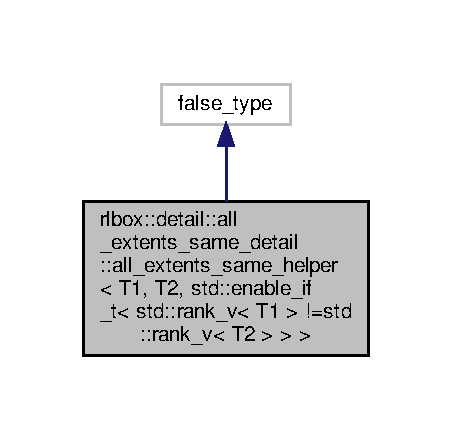
\includegraphics[width=217pt]{structrlbox_1_1detail_1_1all__extents__same__detail_1_1all__extents__same__helper_3_01T1_00_01T22d742f67eff51496871ec1e617d028bb}
\end{center}
\end{figure}


Collaboration diagram for rlbox\+:\+:detail\+:\+:all\+\_\+extents\+\_\+same\+\_\+detail\+:\+:all\+\_\+extents\+\_\+same\+\_\+helper$<$ T1, T2, std\+:\+:enable\+\_\+if\+\_\+t$<$ std\+:\+:rank\+\_\+v$<$ T1 $>$ !=std\+:\+:rank\+\_\+v$<$ T2 $>$ $>$ $>$\+:\nopagebreak
\begin{figure}[H]
\begin{center}
\leavevmode
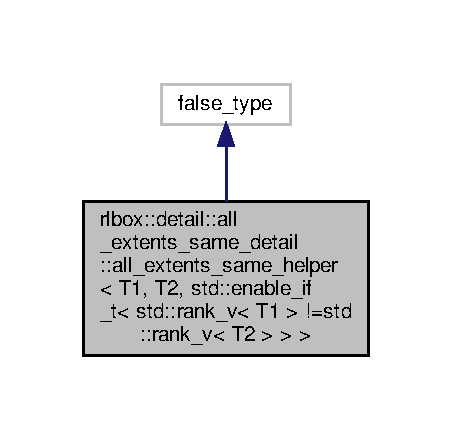
\includegraphics[width=217pt]{structrlbox_1_1detail_1_1all__extents__same__detail_1_1all__extents__same__helper_3_01T1_00_01T27e54e2c89f197b9da103ece8d1864ac7}
\end{center}
\end{figure}


The documentation for this struct was generated from the following file\+:\begin{DoxyCompactItemize}
\item 
/home/shr/\+Code/\+Library\+Sandboxing/rlbox\+\_\+api\+\_\+cpp17/code/include/rlbox\+\_\+type\+\_\+traits.\+hpp\end{DoxyCompactItemize}

\hypertarget{structrlbox_1_1detail_1_1all__extents__same__detail_1_1all__extents__same__helper_3_01T1_00_01T28a926837b387cfc9825b906d80afb9d3}{}\section{rlbox\+:\+:detail\+:\+:all\+\_\+extents\+\_\+same\+\_\+detail\+:\+:all\+\_\+extents\+\_\+same\+\_\+helper$<$ T1, T2, std\+:\+:enable\+\_\+if\+\_\+t$<$ std\+:\+:rank\+\_\+v$<$ T1 $>$==std\+:\+:rank\+\_\+v$<$ T2 $>$ \&\&!std\+:\+:is\+\_\+array\+\_\+v$<$ T1 $>$ \&\&!std\+:\+:is\+\_\+array\+\_\+v$<$ T2 $>$ $>$ $>$ Struct Template Reference}
\label{structrlbox_1_1detail_1_1all__extents__same__detail_1_1all__extents__same__helper_3_01T1_00_01T28a926837b387cfc9825b906d80afb9d3}\index{rlbox\+::detail\+::all\+\_\+extents\+\_\+same\+\_\+detail\+::all\+\_\+extents\+\_\+same\+\_\+helper$<$ T1, T2, std\+::enable\+\_\+if\+\_\+t$<$ std\+::rank\+\_\+v$<$ T1 $>$==std\+::rank\+\_\+v$<$ T2 $>$ \&\&"!std\+::is\+\_\+array\+\_\+v$<$ T1 $>$ \&\&"!std\+::is\+\_\+array\+\_\+v$<$ T2 $>$ $>$ $>$@{rlbox\+::detail\+::all\+\_\+extents\+\_\+same\+\_\+detail\+::all\+\_\+extents\+\_\+same\+\_\+helper$<$ T1, T2, std\+::enable\+\_\+if\+\_\+t$<$ std\+::rank\+\_\+v$<$ T1 $>$==std\+::rank\+\_\+v$<$ T2 $>$ \&\&"!std\+::is\+\_\+array\+\_\+v$<$ T1 $>$ \&\&"!std\+::is\+\_\+array\+\_\+v$<$ T2 $>$ $>$ $>$}}


Inheritance diagram for rlbox\+:\+:detail\+:\+:all\+\_\+extents\+\_\+same\+\_\+detail\+:\+:all\+\_\+extents\+\_\+same\+\_\+helper$<$ T1, T2, std\+:\+:enable\+\_\+if\+\_\+t$<$ std\+:\+:rank\+\_\+v$<$ T1 $>$==std\+:\+:rank\+\_\+v$<$ T2 $>$ \&\&!std\+:\+:is\+\_\+array\+\_\+v$<$ T1 $>$ \&\&!std\+:\+:is\+\_\+array\+\_\+v$<$ T2 $>$ $>$ $>$\+:\nopagebreak
\begin{figure}[H]
\begin{center}
\leavevmode
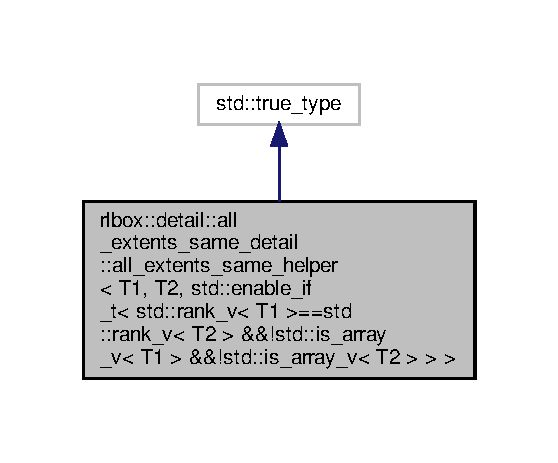
\includegraphics[width=268pt]{structrlbox_1_1detail_1_1all__extents__same__detail_1_1all__extents__same__helper_3_01T1_00_01T2228f0b1f3a6d52754900b3781da85dbb}
\end{center}
\end{figure}


Collaboration diagram for rlbox\+:\+:detail\+:\+:all\+\_\+extents\+\_\+same\+\_\+detail\+:\+:all\+\_\+extents\+\_\+same\+\_\+helper$<$ T1, T2, std\+:\+:enable\+\_\+if\+\_\+t$<$ std\+:\+:rank\+\_\+v$<$ T1 $>$==std\+:\+:rank\+\_\+v$<$ T2 $>$ \&\&!std\+:\+:is\+\_\+array\+\_\+v$<$ T1 $>$ \&\&!std\+:\+:is\+\_\+array\+\_\+v$<$ T2 $>$ $>$ $>$\+:\nopagebreak
\begin{figure}[H]
\begin{center}
\leavevmode
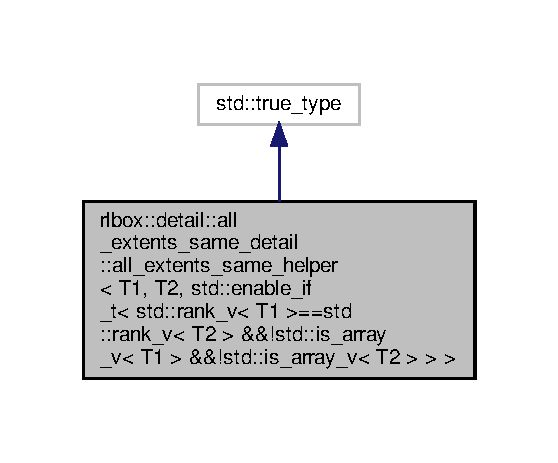
\includegraphics[width=268pt]{structrlbox_1_1detail_1_1all__extents__same__detail_1_1all__extents__same__helper_3_01T1_00_01T2e7958d0f4704c23e1c64420e92977fe8}
\end{center}
\end{figure}


The documentation for this struct was generated from the following file\+:\begin{DoxyCompactItemize}
\item 
/home/shr/\+Code/\+Library\+Sandboxing/rlbox\+\_\+api\+\_\+cpp17/code/include/rlbox\+\_\+type\+\_\+traits.\+hpp\end{DoxyCompactItemize}

\hypertarget{structrlbox_1_1detail_1_1all__extents__same__detail_1_1all__extents__same__helper_3_01T1_00_01T2c85c414d786e56b573ef092d9cd9401b}{}\section{rlbox\+:\+:detail\+:\+:all\+\_\+extents\+\_\+same\+\_\+detail\+:\+:all\+\_\+extents\+\_\+same\+\_\+helper$<$ T1, T2, std\+:\+:enable\+\_\+if\+\_\+t$<$ std\+:\+:rank\+\_\+v$<$ T1 $>$==std\+:\+:rank\+\_\+v$<$ T2 $>$ \&\&std\+:\+:is\+\_\+array\+\_\+v$<$ T1 $>$ \&\&std\+:\+:is\+\_\+array\+\_\+v$<$ T2 $>$ \&\&std\+:\+:extent\+\_\+v$<$ T1 $>$ !=std\+:\+:extent\+\_\+v$<$ T2 $>$ $>$ $>$ Struct Template Reference}
\label{structrlbox_1_1detail_1_1all__extents__same__detail_1_1all__extents__same__helper_3_01T1_00_01T2c85c414d786e56b573ef092d9cd9401b}\index{rlbox\+::detail\+::all\+\_\+extents\+\_\+same\+\_\+detail\+::all\+\_\+extents\+\_\+same\+\_\+helper$<$ T1, T2, std\+::enable\+\_\+if\+\_\+t$<$ std\+::rank\+\_\+v$<$ T1 $>$==std\+::rank\+\_\+v$<$ T2 $>$ \&\&std\+::is\+\_\+array\+\_\+v$<$ T1 $>$ \&\&std\+::is\+\_\+array\+\_\+v$<$ T2 $>$ \&\&std\+::extent\+\_\+v$<$ T1 $>$ "!=std\+::extent\+\_\+v$<$ T2 $>$ $>$ $>$@{rlbox\+::detail\+::all\+\_\+extents\+\_\+same\+\_\+detail\+::all\+\_\+extents\+\_\+same\+\_\+helper$<$ T1, T2, std\+::enable\+\_\+if\+\_\+t$<$ std\+::rank\+\_\+v$<$ T1 $>$==std\+::rank\+\_\+v$<$ T2 $>$ \&\&std\+::is\+\_\+array\+\_\+v$<$ T1 $>$ \&\&std\+::is\+\_\+array\+\_\+v$<$ T2 $>$ \&\&std\+::extent\+\_\+v$<$ T1 $>$ "!=std\+::extent\+\_\+v$<$ T2 $>$ $>$ $>$}}


Inheritance diagram for rlbox\+:\+:detail\+:\+:all\+\_\+extents\+\_\+same\+\_\+detail\+:\+:all\+\_\+extents\+\_\+same\+\_\+helper$<$ T1, T2, std\+:\+:enable\+\_\+if\+\_\+t$<$ std\+:\+:rank\+\_\+v$<$ T1 $>$==std\+:\+:rank\+\_\+v$<$ T2 $>$ \&\&std\+:\+:is\+\_\+array\+\_\+v$<$ T1 $>$ \&\&std\+:\+:is\+\_\+array\+\_\+v$<$ T2 $>$ \&\&std\+:\+:extent\+\_\+v$<$ T1 $>$ !=std\+:\+:extent\+\_\+v$<$ T2 $>$ $>$ $>$\+:
\nopagebreak
\begin{figure}[H]
\begin{center}
\leavevmode
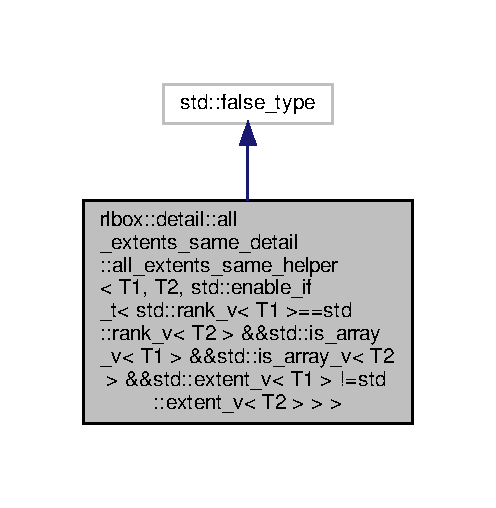
\includegraphics[width=238pt]{structrlbox_1_1detail_1_1all__extents__same__detail_1_1all__extents__same__helper_3_01T1_00_01T2d26e799d2358c1b5289bc704cff16ad5}
\end{center}
\end{figure}


Collaboration diagram for rlbox\+:\+:detail\+:\+:all\+\_\+extents\+\_\+same\+\_\+detail\+:\+:all\+\_\+extents\+\_\+same\+\_\+helper$<$ T1, T2, std\+:\+:enable\+\_\+if\+\_\+t$<$ std\+:\+:rank\+\_\+v$<$ T1 $>$==std\+:\+:rank\+\_\+v$<$ T2 $>$ \&\&std\+:\+:is\+\_\+array\+\_\+v$<$ T1 $>$ \&\&std\+:\+:is\+\_\+array\+\_\+v$<$ T2 $>$ \&\&std\+:\+:extent\+\_\+v$<$ T1 $>$ !=std\+:\+:extent\+\_\+v$<$ T2 $>$ $>$ $>$\+:
\nopagebreak
\begin{figure}[H]
\begin{center}
\leavevmode
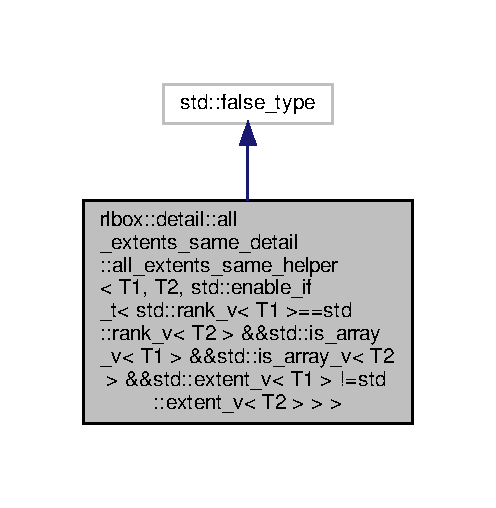
\includegraphics[width=238pt]{structrlbox_1_1detail_1_1all__extents__same__detail_1_1all__extents__same__helper_3_01T1_00_01T2c99e36052fc437e6782967e2a051d51d}
\end{center}
\end{figure}


The documentation for this struct was generated from the following file\+:\begin{DoxyCompactItemize}
\item 
/home/shr/\+Code/\+Library\+Sandboxing/rlbox\+\_\+api\+\_\+cpp17/code/include/rlbox\+\_\+type\+\_\+traits.\+hpp\end{DoxyCompactItemize}

\hypertarget{structrlbox_1_1detail_1_1all__extents__same__detail_1_1all__extents__same__helper_3_01T1_00_01T2dafdc234639e9e1d414a62f1ef1ccd73}{}\section{rlbox\+:\+:detail\+:\+:all\+\_\+extents\+\_\+same\+\_\+detail\+:\+:all\+\_\+extents\+\_\+same\+\_\+helper$<$ T1, T2, std\+:\+:enable\+\_\+if\+\_\+t$<$ std\+:\+:rank\+\_\+v$<$ T1 $>$==std\+:\+:rank\+\_\+v$<$ T2 $>$ \&\&std\+:\+:is\+\_\+array\+\_\+v$<$ T1 $>$ \&\&std\+:\+:is\+\_\+array\+\_\+v$<$ T2 $>$ \&\&std\+:\+:extent\+\_\+v$<$ T1 $>$==std\+:\+:extent\+\_\+v$<$ T2 $>$ $>$ $>$ Struct Template Reference}
\label{structrlbox_1_1detail_1_1all__extents__same__detail_1_1all__extents__same__helper_3_01T1_00_01T2dafdc234639e9e1d414a62f1ef1ccd73}\index{rlbox\+::detail\+::all\+\_\+extents\+\_\+same\+\_\+detail\+::all\+\_\+extents\+\_\+same\+\_\+helper$<$ T1, T2, std\+::enable\+\_\+if\+\_\+t$<$ std\+::rank\+\_\+v$<$ T1 $>$==std\+::rank\+\_\+v$<$ T2 $>$ \&\&std\+::is\+\_\+array\+\_\+v$<$ T1 $>$ \&\&std\+::is\+\_\+array\+\_\+v$<$ T2 $>$ \&\&std\+::extent\+\_\+v$<$ T1 $>$==std\+::extent\+\_\+v$<$ T2 $>$ $>$ $>$@{rlbox\+::detail\+::all\+\_\+extents\+\_\+same\+\_\+detail\+::all\+\_\+extents\+\_\+same\+\_\+helper$<$ T1, T2, std\+::enable\+\_\+if\+\_\+t$<$ std\+::rank\+\_\+v$<$ T1 $>$==std\+::rank\+\_\+v$<$ T2 $>$ \&\&std\+::is\+\_\+array\+\_\+v$<$ T1 $>$ \&\&std\+::is\+\_\+array\+\_\+v$<$ T2 $>$ \&\&std\+::extent\+\_\+v$<$ T1 $>$==std\+::extent\+\_\+v$<$ T2 $>$ $>$ $>$}}
\subsection*{Static Public Attributes}
\begin{DoxyCompactItemize}
\item 
static constexpr bool {\bfseries value}
\end{DoxyCompactItemize}


\subsection{Member Data Documentation}
\mbox{\Hypertarget{structrlbox_1_1detail_1_1all__extents__same__detail_1_1all__extents__same__helper_3_01T1_00_01T2dafdc234639e9e1d414a62f1ef1ccd73_a62e8d74da3bfda38a748a6767206723a}\label{structrlbox_1_1detail_1_1all__extents__same__detail_1_1all__extents__same__helper_3_01T1_00_01T2dafdc234639e9e1d414a62f1ef1ccd73_a62e8d74da3bfda38a748a6767206723a}} 
\index{rlbox\+::detail\+::all\+\_\+extents\+\_\+same\+\_\+detail\+::all\+\_\+extents\+\_\+same\+\_\+helper$<$ T1, T2, std\+::enable\+\_\+if\+\_\+t$<$ std\+::rank\+\_\+v$<$ T1 $>$==std\+::rank\+\_\+v$<$ T2 $>$ \&\&std\+::is\+\_\+array\+\_\+v$<$ T1 $>$ \&\&std\+::is\+\_\+array\+\_\+v$<$ T2 $>$ \&\&std\+::extent\+\_\+v$<$ T1 $>$==std\+::extent\+\_\+v$<$ T2 $>$ $>$ $>$@{rlbox\+::detail\+::all\+\_\+extents\+\_\+same\+\_\+detail\+::all\+\_\+extents\+\_\+same\+\_\+helper$<$ T1, T2, std\+::enable\+\_\+if\+\_\+t$<$ std\+::rank\+\_\+v$<$ T1 $>$==std\+::rank\+\_\+v$<$ T2 $>$ \&\&std\+::is\+\_\+array\+\_\+v$<$ T1 $>$ \&\&std\+::is\+\_\+array\+\_\+v$<$ T2 $>$ \&\&std\+::extent\+\_\+v$<$ T1 $>$==std\+::extent\+\_\+v$<$ T2 $>$ $>$ $>$}!value@{value}}
\index{value@{value}!rlbox\+::detail\+::all\+\_\+extents\+\_\+same\+\_\+detail\+::all\+\_\+extents\+\_\+same\+\_\+helper$<$ T1, T2, std\+::enable\+\_\+if\+\_\+t$<$ std\+::rank\+\_\+v$<$ T1 $>$==std\+::rank\+\_\+v$<$ T2 $>$ \&\&std\+::is\+\_\+array\+\_\+v$<$ T1 $>$ \&\&std\+::is\+\_\+array\+\_\+v$<$ T2 $>$ \&\&std\+::extent\+\_\+v$<$ T1 $>$==std\+::extent\+\_\+v$<$ T2 $>$ $>$ $>$@{rlbox\+::detail\+::all\+\_\+extents\+\_\+same\+\_\+detail\+::all\+\_\+extents\+\_\+same\+\_\+helper$<$ T1, T2, std\+::enable\+\_\+if\+\_\+t$<$ std\+::rank\+\_\+v$<$ T1 $>$==std\+::rank\+\_\+v$<$ T2 $>$ \&\&std\+::is\+\_\+array\+\_\+v$<$ T1 $>$ \&\&std\+::is\+\_\+array\+\_\+v$<$ T2 $>$ \&\&std\+::extent\+\_\+v$<$ T1 $>$==std\+::extent\+\_\+v$<$ T2 $>$ $>$ $>$}}
\subsubsection{\texorpdfstring{value}{value}}
{\footnotesize\ttfamily template$<$typename T1 , typename T2 $>$ \\
constexpr bool \hyperlink{structrlbox_1_1detail_1_1all__extents__same__detail_1_1all__extents__same__helper}{rlbox\+::detail\+::all\+\_\+extents\+\_\+same\+\_\+detail\+::all\+\_\+extents\+\_\+same\+\_\+helper}$<$ T1, T2, std\+::enable\+\_\+if\+\_\+t$<$ std\+::rank\+\_\+v$<$ T1 $>$==std\+::rank\+\_\+v$<$ T2 $>$ \&\&std\+::is\+\_\+array\+\_\+v$<$ T1 $>$ \&\&std\+::is\+\_\+array\+\_\+v$<$ T2 $>$ \&\&std\+::extent\+\_\+v$<$ T1 $>$==std\+::extent\+\_\+v$<$ T2 $>$ $>$ $>$\+::value\hspace{0.3cm}{\ttfamily [static]}}

{\bfseries Initial value\+:}
\begin{DoxyCode}
=
      all\_extents\_same\_helper<std::remove\_extent\_t<T1>,
                              std::remove\_extent\_t<T2>>::value
\end{DoxyCode}


The documentation for this struct was generated from the following file\+:\begin{DoxyCompactItemize}
\item 
/home/shr/\+Code/\+Library\+Sandboxing/rlbox\+\_\+api\+\_\+cpp17/code/include/rlbox\+\_\+type\+\_\+traits.\+hpp\end{DoxyCompactItemize}

\hypertarget{structrlbox_1_1detail_1_1base__type__detail_1_1base__type}{}\doxysection{rlbox\+::detail\+::base\+\_\+type\+\_\+detail\+::base\+\_\+type$<$ T $>$ Struct Template Reference}
\label{structrlbox_1_1detail_1_1base__type__detail_1_1base__type}\index{rlbox::detail::base\_type\_detail::base\_type$<$ T $>$@{rlbox::detail::base\_type\_detail::base\_type$<$ T $>$}}
\doxysubsection*{Public Types}
\begin{DoxyCompactItemize}
\item 
\mbox{\Hypertarget{structrlbox_1_1detail_1_1base__type__detail_1_1base__type_af9466e26bc26b30bd00bf9361b163813}\label{structrlbox_1_1detail_1_1base__type__detail_1_1base__type_af9466e26bc26b30bd00bf9361b163813}} 
typedef T {\bfseries type}
\end{DoxyCompactItemize}


The documentation for this struct was generated from the following file\+:\begin{DoxyCompactItemize}
\item 
/home/shr/\+Code/\+Library\+Sandboxing/rlbox\+\_\+api\+\_\+cpp17/code/include/rlbox\+\_\+type\+\_\+traits.\+hpp\end{DoxyCompactItemize}

\hypertarget{structrlbox_1_1detail_1_1base__type__detail_1_1base__type_3_01T_01_5_01_4}{}\doxysection{rlbox\+::detail\+::base\+\_\+type\+\_\+detail\+::base\+\_\+type\texorpdfstring{$<$}{<} T $\ast$ \texorpdfstring{$>$}{>} Struct Template Reference}
\label{structrlbox_1_1detail_1_1base__type__detail_1_1base__type_3_01T_01_5_01_4}\index{rlbox::detail::base\_type\_detail::base\_type$<$ T $\ast$ $>$@{rlbox::detail::base\_type\_detail::base\_type$<$ T $\ast$ $>$}}
\doxysubsection*{Public Types}
\begin{DoxyCompactItemize}
\item 
\mbox{\Hypertarget{structrlbox_1_1detail_1_1base__type__detail_1_1base__type_3_01T_01_5_01_4_a887e34c81c8f29a04ee6247929ac4699}\label{structrlbox_1_1detail_1_1base__type__detail_1_1base__type_3_01T_01_5_01_4_a887e34c81c8f29a04ee6247929ac4699}} 
typedef \mbox{\hyperlink{structrlbox_1_1detail_1_1base__type__detail_1_1base__type}{base\+\_\+type}}$<$ T $>$\+::type {\bfseries type}
\end{DoxyCompactItemize}


The documentation for this struct was generated from the following file\+:\begin{DoxyCompactItemize}
\item 
/home/d/hack/rlbox\+\_\+sandboxing\+\_\+api/code/include/rlbox\+\_\+type\+\_\+traits.\+hpp\end{DoxyCompactItemize}

\hypertarget{structrlbox_1_1detail_1_1base__type__detail_1_1base__type_3_01T[]_4}{}\section{rlbox\+:\+:detail\+:\+:base\+\_\+type\+\_\+detail\+:\+:base\+\_\+type$<$ T\mbox{[}\mbox{]}$>$ Struct Template Reference}
\label{structrlbox_1_1detail_1_1base__type__detail_1_1base__type_3_01T[]_4}\index{rlbox\+::detail\+::base\+\_\+type\+\_\+detail\+::base\+\_\+type$<$ T\mbox{[}\mbox{]}$>$@{rlbox\+::detail\+::base\+\_\+type\+\_\+detail\+::base\+\_\+type$<$ T[]$>$}}
\subsection*{Public Types}
\begin{DoxyCompactItemize}
\item 
\mbox{\Hypertarget{structrlbox_1_1detail_1_1base__type__detail_1_1base__type_3_01T[]_4_a9d9664258521223ed1debcd068852a54}\label{structrlbox_1_1detail_1_1base__type__detail_1_1base__type_3_01T[]_4_a9d9664258521223ed1debcd068852a54}} 
typedef \hyperlink{structrlbox_1_1detail_1_1base__type__detail_1_1base__type}{base\+\_\+type}$<$ T $>$\+::type {\bfseries type}
\end{DoxyCompactItemize}


The documentation for this struct was generated from the following file\+:\begin{DoxyCompactItemize}
\item 
/home/shr/\+Code/\+Library\+Sandboxing/rlbox\+\_\+api\+\_\+cpp17/code/include/rlbox\+\_\+type\+\_\+traits.\+hpp\end{DoxyCompactItemize}

\hypertarget{structrlbox_1_1detail_1_1base__type__detail_1_1base__type_3_01T[N]_4}{}\section{rlbox\+:\+:detail\+:\+:base\+\_\+type\+\_\+detail\+:\+:base\+\_\+type$<$ T\mbox{[}N\mbox{]}$>$ Struct Template Reference}
\label{structrlbox_1_1detail_1_1base__type__detail_1_1base__type_3_01T[N]_4}\index{rlbox\+::detail\+::base\+\_\+type\+\_\+detail\+::base\+\_\+type$<$ T\mbox{[}N\mbox{]}$>$@{rlbox\+::detail\+::base\+\_\+type\+\_\+detail\+::base\+\_\+type$<$ T[N]$>$}}
\subsection*{Public Types}
\begin{DoxyCompactItemize}
\item 
\mbox{\Hypertarget{structrlbox_1_1detail_1_1base__type__detail_1_1base__type_3_01T[N]_4_ac0c6aec36bdd840ebb83930c497f7e5f}\label{structrlbox_1_1detail_1_1base__type__detail_1_1base__type_3_01T[N]_4_ac0c6aec36bdd840ebb83930c497f7e5f}} 
typedef \hyperlink{structrlbox_1_1detail_1_1base__type__detail_1_1base__type}{base\+\_\+type}$<$ T $>$\+::type {\bfseries type}
\end{DoxyCompactItemize}


The documentation for this struct was generated from the following file\+:\begin{DoxyCompactItemize}
\item 
/home/shr/\+Code/\+Library\+Sandboxing/rlbox\+\_\+api\+\_\+cpp17/code/include/rlbox\+\_\+type\+\_\+traits.\+hpp\end{DoxyCompactItemize}

\hypertarget{structrlbox_1_1detail_1_1convert__detail_1_1convert__base__types__t__helper}{}\doxysection{rlbox\+::detail\+::convert\+\_\+detail\+::convert\+\_\+base\+\_\+types\+\_\+t\+\_\+helper$<$ T, T\+\_\+\+Short\+Type, T\+\_\+\+Int\+Type, T\+\_\+\+Long\+Type, T\+\_\+\+Long\+Long\+Type, T\+\_\+\+Pointer\+Type, T\+\_\+\+Enable $>$ Struct Template Reference}
\label{structrlbox_1_1detail_1_1convert__detail_1_1convert__base__types__t__helper}\index{rlbox::detail::convert\_detail::convert\_base\_types\_t\_helper$<$ T, T\_ShortType, T\_IntType, T\_LongType, T\_LongLongType, T\_PointerType, T\_Enable $>$@{rlbox::detail::convert\_detail::convert\_base\_types\_t\_helper$<$ T, T\_ShortType, T\_IntType, T\_LongType, T\_LongLongType, T\_PointerType, T\_Enable $>$}}


The documentation for this struct was generated from the following file\+:\begin{DoxyCompactItemize}
\item 
/home/d/hack/rlbox\+\_\+sandboxing\+\_\+api/code/include/rlbox\+\_\+type\+\_\+traits.\+hpp\end{DoxyCompactItemize}

\hypertarget{structrlbox_1_1detail_1_1convert__detail_1_1convert__base__types__t__helper_3_01T_00_01T__ShortT9669a45f33d18c9be6a22efe2b66d10c}{}\doxysection{rlbox\+::detail\+::convert\+\_\+detail\+::convert\+\_\+base\+\_\+types\+\_\+t\+\_\+helper$<$ T, T\+\_\+\+Short\+Type, T\+\_\+\+Int\+Type, T\+\_\+\+Long\+Type, T\+\_\+\+Long\+Long\+Type, T\+\_\+\+Pointer\+Type, std\+::enable\+\_\+if\+\_\+t$<$ std\+::is\+\_\+array\+\_\+v$<$ T $>$ \&\&!std\+::is\+\_\+const\+\_\+v$<$ T $>$ $>$ $>$ Struct Template Reference}
\label{structrlbox_1_1detail_1_1convert__detail_1_1convert__base__types__t__helper_3_01T_00_01T__ShortT9669a45f33d18c9be6a22efe2b66d10c}\index{rlbox::detail::convert\_detail::convert\_base\_types\_t\_helper$<$ T, T\_ShortType, T\_IntType, T\_LongType, T\_LongLongType, T\_PointerType, std::enable\_if\_t$<$ std::is\_array\_v$<$ T $>$ \&\&"!std::is\_const\_v$<$ T $>$ $>$ $>$@{rlbox::detail::convert\_detail::convert\_base\_types\_t\_helper$<$ T, T\_ShortType, T\_IntType, T\_LongType, T\_LongLongType, T\_PointerType, std::enable\_if\_t$<$ std::is\_array\_v$<$ T $>$ \&\&"!std::is\_const\_v$<$ T $>$ $>$ $>$}}
\doxysubsection*{Public Types}
\begin{DoxyCompactItemize}
\item 
\mbox{\Hypertarget{structrlbox_1_1detail_1_1convert__detail_1_1convert__base__types__t__helper_3_01T_00_01T__ShortT9669a45f33d18c9be6a22efe2b66d10c_a502367a191bcee084370b22af09dd63e}\label{structrlbox_1_1detail_1_1convert__detail_1_1convert__base__types__t__helper_3_01T_00_01T__ShortT9669a45f33d18c9be6a22efe2b66d10c_a502367a191bcee084370b22af09dd63e}} 
using {\bfseries type} = typename \mbox{\hyperlink{structrlbox_1_1detail_1_1convert__detail_1_1convert__base__types__t__helper}{convert\+\_\+base\+\_\+types\+\_\+t\+\_\+helper}}$<$ std\+::remove\+\_\+extent\+\_\+t$<$ T $>$, T\+\_\+\+Short\+Type, T\+\_\+\+Int\+Type, T\+\_\+\+Long\+Type, T\+\_\+\+Long\+Long\+Type, T\+\_\+\+Pointer\+Type $>$\+::type\mbox{[}std\+::extent\+\_\+v$<$ T $>$\mbox{]}
\end{DoxyCompactItemize}


The documentation for this struct was generated from the following file\+:\begin{DoxyCompactItemize}
\item 
/home/d/hack/rlbox\+\_\+api\+\_\+cpp17/code/include/rlbox\+\_\+type\+\_\+traits.\+hpp\end{DoxyCompactItemize}

\hypertarget{structrlbox_1_1detail_1_1convert__detail_1_1convert__base__types__t__helper_3_01T_00_01T__ShortTc61ef72b6a1c5b4e6ef41be35597aa72}{}\doxysection{rlbox\+::detail\+::convert\+\_\+detail\+::convert\+\_\+base\+\_\+types\+\_\+t\+\_\+helper$<$ T, T\+\_\+\+Short\+Type, T\+\_\+\+Int\+Type, T\+\_\+\+Long\+Type, T\+\_\+\+Long\+Long\+Type, T\+\_\+\+Pointer\+Type, std\+::enable\+\_\+if\+\_\+t$<$ std\+::is\+\_\+const\+\_\+v$<$ T $>$ $>$ $>$ Struct Template Reference}
\label{structrlbox_1_1detail_1_1convert__detail_1_1convert__base__types__t__helper_3_01T_00_01T__ShortTc61ef72b6a1c5b4e6ef41be35597aa72}\index{rlbox::detail::convert\_detail::convert\_base\_types\_t\_helper$<$ T, T\_ShortType, T\_IntType, T\_LongType, T\_LongLongType, T\_PointerType, std::enable\_if\_t$<$ std::is\_const\_v$<$ T $>$ $>$ $>$@{rlbox::detail::convert\_detail::convert\_base\_types\_t\_helper$<$ T, T\_ShortType, T\_IntType, T\_LongType, T\_LongLongType, T\_PointerType, std::enable\_if\_t$<$ std::is\_const\_v$<$ T $>$ $>$ $>$}}
\doxysubsection*{Public Types}
\begin{DoxyCompactItemize}
\item 
\mbox{\Hypertarget{structrlbox_1_1detail_1_1convert__detail_1_1convert__base__types__t__helper_3_01T_00_01T__ShortTc61ef72b6a1c5b4e6ef41be35597aa72_af4d9297decb84433598acbe0c0b2d94f}\label{structrlbox_1_1detail_1_1convert__detail_1_1convert__base__types__t__helper_3_01T_00_01T__ShortTc61ef72b6a1c5b4e6ef41be35597aa72_af4d9297decb84433598acbe0c0b2d94f}} 
using {\bfseries type} = std\+::add\+\_\+const\+\_\+t$<$ typename \mbox{\hyperlink{structrlbox_1_1detail_1_1convert__detail_1_1convert__base__types__t__helper}{convert\+\_\+base\+\_\+types\+\_\+t\+\_\+helper}}$<$ std\+::remove\+\_\+const\+\_\+t$<$ T $>$, T\+\_\+\+Short\+Type, T\+\_\+\+Int\+Type, T\+\_\+\+Long\+Type, T\+\_\+\+Long\+Long\+Type, T\+\_\+\+Pointer\+Type $>$\+::type $>$
\end{DoxyCompactItemize}


The documentation for this struct was generated from the following file\+:\begin{DoxyCompactItemize}
\item 
/home/d/hack/rlbox\+\_\+sandboxing\+\_\+api/code/include/rlbox\+\_\+type\+\_\+traits.\+hpp\end{DoxyCompactItemize}

\hypertarget{structrlbox_1_1detail_1_1convert__detail_1_1convert__base__types__t__helper_3_01T_00_01T__ShortT47d1caaebe2e5bd6a334ab7184ad13c2}{}\doxysection{rlbox\+::detail\+::convert\+\_\+detail\+::convert\+\_\+base\+\_\+types\+\_\+t\+\_\+helper\texorpdfstring{$<$}{<} T, T\+\_\+\+Short\+Type, T\+\_\+\+Int\+Type, T\+\_\+\+Long\+Type, T\+\_\+\+Long\+Long\+Type, T\+\_\+\+Pointer\+Type, std\+::enable\+\_\+if\+\_\+t\texorpdfstring{$<$}{<} std\+::is\+\_\+pointer\+\_\+v\texorpdfstring{$<$}{<} T \texorpdfstring{$>$}{>} \&\&!std\+::is\+\_\+const\+\_\+v\texorpdfstring{$<$}{<} T \texorpdfstring{$>$}{>} \texorpdfstring{$>$}{>} \texorpdfstring{$>$}{>} Struct Template Reference}
\label{structrlbox_1_1detail_1_1convert__detail_1_1convert__base__types__t__helper_3_01T_00_01T__ShortT47d1caaebe2e5bd6a334ab7184ad13c2}\index{rlbox::detail::convert\_detail::convert\_base\_types\_t\_helper$<$ T, T\_ShortType, T\_IntType, T\_LongType, T\_LongLongType, T\_PointerType, std::enable\_if\_t$<$ std::is\_pointer\_v$<$ T $>$ \&\&"!std::is\_const\_v$<$ T $>$ $>$ $>$@{rlbox::detail::convert\_detail::convert\_base\_types\_t\_helper$<$ T, T\_ShortType, T\_IntType, T\_LongType, T\_LongLongType, T\_PointerType, std::enable\_if\_t$<$ std::is\_pointer\_v$<$ T $>$ \&\&"!std::is\_const\_v$<$ T $>$ $>$ $>$}}
\doxysubsection*{Public Types}
\begin{DoxyCompactItemize}
\item 
\mbox{\Hypertarget{structrlbox_1_1detail_1_1convert__detail_1_1convert__base__types__t__helper_3_01T_00_01T__ShortT47d1caaebe2e5bd6a334ab7184ad13c2_a1b6604639291d981ec73c1fb959e60ea}\label{structrlbox_1_1detail_1_1convert__detail_1_1convert__base__types__t__helper_3_01T_00_01T__ShortT47d1caaebe2e5bd6a334ab7184ad13c2_a1b6604639291d981ec73c1fb959e60ea}} 
using {\bfseries type} = T\+\_\+\+Pointer\+Type
\end{DoxyCompactItemize}


The documentation for this struct was generated from the following file\+:\begin{DoxyCompactItemize}
\item 
/home/d/hack/rlbox\+\_\+sandboxing\+\_\+api/code/include/rlbox\+\_\+type\+\_\+traits.\+hpp\end{DoxyCompactItemize}

\hypertarget{structrlbox_1_1detail_1_1convert__detail_1_1convert__base__types__t__helper_3_01T_00_01T__ShortTc2ed7d8e5c23ce6ae87cc658a172a860}{}\doxysection{rlbox\+::detail\+::convert\+\_\+detail\+::convert\+\_\+base\+\_\+types\+\_\+t\+\_\+helper$<$ T, T\+\_\+\+Short\+Type, T\+\_\+\+Int\+Type, T\+\_\+\+Long\+Type, T\+\_\+\+Long\+Long\+Type, T\+\_\+\+Pointer\+Type, std\+::enable\+\_\+if\+\_\+t$<$ std\+::is\+\_\+same\+\_\+v$<$ int, T $>$ \&\&!std\+::is\+\_\+const\+\_\+v$<$ T $>$ $>$ $>$ Struct Template Reference}
\label{structrlbox_1_1detail_1_1convert__detail_1_1convert__base__types__t__helper_3_01T_00_01T__ShortTc2ed7d8e5c23ce6ae87cc658a172a860}\index{rlbox::detail::convert\_detail::convert\_base\_types\_t\_helper$<$ T, T\_ShortType, T\_IntType, T\_LongType, T\_LongLongType, T\_PointerType, std::enable\_if\_t$<$ std::is\_same\_v$<$ int, T $>$ \&\&"!std::is\_const\_v$<$ T $>$ $>$ $>$@{rlbox::detail::convert\_detail::convert\_base\_types\_t\_helper$<$ T, T\_ShortType, T\_IntType, T\_LongType, T\_LongLongType, T\_PointerType, std::enable\_if\_t$<$ std::is\_same\_v$<$ int, T $>$ \&\&"!std::is\_const\_v$<$ T $>$ $>$ $>$}}
\doxysubsection*{Public Types}
\begin{DoxyCompactItemize}
\item 
\mbox{\Hypertarget{structrlbox_1_1detail_1_1convert__detail_1_1convert__base__types__t__helper_3_01T_00_01T__ShortTc2ed7d8e5c23ce6ae87cc658a172a860_a883107aeae87db2a750b0da49414ccb2}\label{structrlbox_1_1detail_1_1convert__detail_1_1convert__base__types__t__helper_3_01T_00_01T__ShortTc2ed7d8e5c23ce6ae87cc658a172a860_a883107aeae87db2a750b0da49414ccb2}} 
using {\bfseries type} = T\+\_\+\+Int\+Type
\end{DoxyCompactItemize}


The documentation for this struct was generated from the following file\+:\begin{DoxyCompactItemize}
\item 
/home/d/hack/rlbox\+\_\+sandboxing\+\_\+api/code/include/rlbox\+\_\+type\+\_\+traits.\+hpp\end{DoxyCompactItemize}

\hypertarget{structrlbox_1_1detail_1_1convert__detail_1_1convert__base__types__t__helper_3_01T_00_01T__ShortTfd6b32b52e4b70d0e9d13d00bd744f5b}{}\doxysection{rlbox\+::detail\+::convert\+\_\+detail\+::convert\+\_\+base\+\_\+types\+\_\+t\+\_\+helper$<$ T, T\+\_\+\+Short\+Type, T\+\_\+\+Int\+Type, T\+\_\+\+Long\+Type, T\+\_\+\+Long\+Long\+Type, T\+\_\+\+Pointer\+Type, std\+::enable\+\_\+if\+\_\+t$<$ std\+::is\+\_\+same\+\_\+v$<$ long long, T $>$ \&\&!std\+::is\+\_\+const\+\_\+v$<$ T $>$ $>$ $>$ Struct Template Reference}
\label{structrlbox_1_1detail_1_1convert__detail_1_1convert__base__types__t__helper_3_01T_00_01T__ShortTfd6b32b52e4b70d0e9d13d00bd744f5b}\index{rlbox::detail::convert\_detail::convert\_base\_types\_t\_helper$<$ T, T\_ShortType, T\_IntType, T\_LongType, T\_LongLongType, T\_PointerType, std::enable\_if\_t$<$ std::is\_same\_v$<$ long long, T $>$ \&\&"!std::is\_const\_v$<$ T $>$ $>$ $>$@{rlbox::detail::convert\_detail::convert\_base\_types\_t\_helper$<$ T, T\_ShortType, T\_IntType, T\_LongType, T\_LongLongType, T\_PointerType, std::enable\_if\_t$<$ std::is\_same\_v$<$ long long, T $>$ \&\&"!std::is\_const\_v$<$ T $>$ $>$ $>$}}
\doxysubsection*{Public Types}
\begin{DoxyCompactItemize}
\item 
\mbox{\Hypertarget{structrlbox_1_1detail_1_1convert__detail_1_1convert__base__types__t__helper_3_01T_00_01T__ShortTfd6b32b52e4b70d0e9d13d00bd744f5b_a42b9947572f7bab2ff3a99f73af00f44}\label{structrlbox_1_1detail_1_1convert__detail_1_1convert__base__types__t__helper_3_01T_00_01T__ShortTfd6b32b52e4b70d0e9d13d00bd744f5b_a42b9947572f7bab2ff3a99f73af00f44}} 
using {\bfseries type} = T\+\_\+\+Long\+Long\+Type
\end{DoxyCompactItemize}


The documentation for this struct was generated from the following file\+:\begin{DoxyCompactItemize}
\item 
/home/shr/\+Code/\+Library\+Sandboxing/rlbox\+\_\+api\+\_\+cpp17/code/include/rlbox\+\_\+type\+\_\+traits.\+hpp\end{DoxyCompactItemize}

\hypertarget{structrlbox_1_1detail_1_1convert__detail_1_1convert__base__types__t__helper_3_01T_00_01T__ShortT956ceb54575cc1a39f8f361203064da2}{}\section{rlbox\+:\+:detail\+:\+:convert\+\_\+detail\+:\+:convert\+\_\+base\+\_\+types\+\_\+t\+\_\+helper$<$ T, T\+\_\+\+Short\+Type, T\+\_\+\+Int\+Type, T\+\_\+\+Long\+Type, T\+\_\+\+Long\+Long\+Type, T\+\_\+\+Pointer\+Type, std\+:\+:enable\+\_\+if\+\_\+t$<$ std\+:\+:is\+\_\+same\+\_\+v$<$ long, T $>$ \&\&!std\+:\+:is\+\_\+const\+\_\+v$<$ T $>$ $>$ $>$ Struct Template Reference}
\label{structrlbox_1_1detail_1_1convert__detail_1_1convert__base__types__t__helper_3_01T_00_01T__ShortT956ceb54575cc1a39f8f361203064da2}\index{rlbox\+::detail\+::convert\+\_\+detail\+::convert\+\_\+base\+\_\+types\+\_\+t\+\_\+helper$<$ T, T\+\_\+\+Short\+Type, T\+\_\+\+Int\+Type, T\+\_\+\+Long\+Type, T\+\_\+\+Long\+Long\+Type, T\+\_\+\+Pointer\+Type, std\+::enable\+\_\+if\+\_\+t$<$ std\+::is\+\_\+same\+\_\+v$<$ long, T $>$ \&\&"!std\+::is\+\_\+const\+\_\+v$<$ T $>$ $>$ $>$@{rlbox\+::detail\+::convert\+\_\+detail\+::convert\+\_\+base\+\_\+types\+\_\+t\+\_\+helper$<$ T, T\+\_\+\+Short\+Type, T\+\_\+\+Int\+Type, T\+\_\+\+Long\+Type, T\+\_\+\+Long\+Long\+Type, T\+\_\+\+Pointer\+Type, std\+::enable\+\_\+if\+\_\+t$<$ std\+::is\+\_\+same\+\_\+v$<$ long, T $>$ \&\&"!std\+::is\+\_\+const\+\_\+v$<$ T $>$ $>$ $>$}}
\subsection*{Public Types}
\begin{DoxyCompactItemize}
\item 
\mbox{\Hypertarget{structrlbox_1_1detail_1_1convert__detail_1_1convert__base__types__t__helper_3_01T_00_01T__ShortT956ceb54575cc1a39f8f361203064da2_accfbaf521e8181f1aa9cf484c703905c}\label{structrlbox_1_1detail_1_1convert__detail_1_1convert__base__types__t__helper_3_01T_00_01T__ShortT956ceb54575cc1a39f8f361203064da2_accfbaf521e8181f1aa9cf484c703905c}} 
using {\bfseries type} = T\+\_\+\+Long\+Type
\end{DoxyCompactItemize}


The documentation for this struct was generated from the following file\+:\begin{DoxyCompactItemize}
\item 
/home/shr/\+Code/\+Library\+Sandboxing/rlbox\+\_\+api\+\_\+cpp17/code/include/rlbox\+\_\+type\+\_\+traits.\+hpp\end{DoxyCompactItemize}

\hypertarget{structrlbox_1_1detail_1_1convert__detail_1_1convert__base__types__t__helper_3_01T_00_01T__ShortTd09a1c93590178c260005e6430499871}{}\doxysection{rlbox\+::detail\+::convert\+\_\+detail\+::convert\+\_\+base\+\_\+types\+\_\+t\+\_\+helper\texorpdfstring{$<$}{<} T, T\+\_\+\+Short\+Type, T\+\_\+\+Int\+Type, T\+\_\+\+Long\+Type, T\+\_\+\+Long\+Long\+Type, T\+\_\+\+Pointer\+Type, std\+::enable\+\_\+if\+\_\+t\texorpdfstring{$<$}{<} std\+::is\+\_\+same\+\_\+v\texorpdfstring{$<$}{<} short, T \texorpdfstring{$>$}{>} \&\&!std\+::is\+\_\+const\+\_\+v\texorpdfstring{$<$}{<} T \texorpdfstring{$>$}{>} \texorpdfstring{$>$}{>} \texorpdfstring{$>$}{>} Struct Template Reference}
\label{structrlbox_1_1detail_1_1convert__detail_1_1convert__base__types__t__helper_3_01T_00_01T__ShortTd09a1c93590178c260005e6430499871}\index{rlbox::detail::convert\_detail::convert\_base\_types\_t\_helper$<$ T, T\_ShortType, T\_IntType, T\_LongType, T\_LongLongType, T\_PointerType, std::enable\_if\_t$<$ std::is\_same\_v$<$ short, T $>$ \&\&"!std::is\_const\_v$<$ T $>$ $>$ $>$@{rlbox::detail::convert\_detail::convert\_base\_types\_t\_helper$<$ T, T\_ShortType, T\_IntType, T\_LongType, T\_LongLongType, T\_PointerType, std::enable\_if\_t$<$ std::is\_same\_v$<$ short, T $>$ \&\&"!std::is\_const\_v$<$ T $>$ $>$ $>$}}
\doxysubsection*{Public Types}
\begin{DoxyCompactItemize}
\item 
\mbox{\Hypertarget{structrlbox_1_1detail_1_1convert__detail_1_1convert__base__types__t__helper_3_01T_00_01T__ShortTd09a1c93590178c260005e6430499871_acc928cabc40780bf019da1735727cd2a}\label{structrlbox_1_1detail_1_1convert__detail_1_1convert__base__types__t__helper_3_01T_00_01T__ShortTd09a1c93590178c260005e6430499871_acc928cabc40780bf019da1735727cd2a}} 
using {\bfseries type} = T\+\_\+\+Short\+Type
\end{DoxyCompactItemize}


The documentation for this struct was generated from the following file\+:\begin{DoxyCompactItemize}
\item 
/home/d/hack/rlbox\+\_\+sandboxing\+\_\+api/code/include/rlbox\+\_\+type\+\_\+traits.\+hpp\end{DoxyCompactItemize}

\hypertarget{structrlbox_1_1detail_1_1convert__detail_1_1convert__base__types__t__helper_3_01T_00_01T__ShortT2bc89571370fe560fd1dec2752f78995}{}\section{rlbox\+:\+:detail\+:\+:convert\+\_\+detail\+:\+:convert\+\_\+base\+\_\+types\+\_\+t\+\_\+helper$<$ T, T\+\_\+\+Short\+Type, T\+\_\+\+Int\+Type, T\+\_\+\+Long\+Type, T\+\_\+\+Long\+Long\+Type, T\+\_\+\+Pointer\+Type, std\+:\+:enable\+\_\+if\+\_\+t$<$ std\+:\+:is\+\_\+unsigned\+\_\+v$<$ T $>$ \&\&!std\+:\+:is\+\_\+same\+\_\+v$<$ T, bool $>$ \&\&!std\+:\+:is\+\_\+const\+\_\+v$<$ T $>$ $>$ $>$ Struct Template Reference}
\label{structrlbox_1_1detail_1_1convert__detail_1_1convert__base__types__t__helper_3_01T_00_01T__ShortT2bc89571370fe560fd1dec2752f78995}\index{rlbox\+::detail\+::convert\+\_\+detail\+::convert\+\_\+base\+\_\+types\+\_\+t\+\_\+helper$<$ T, T\+\_\+\+Short\+Type, T\+\_\+\+Int\+Type, T\+\_\+\+Long\+Type, T\+\_\+\+Long\+Long\+Type, T\+\_\+\+Pointer\+Type, std\+::enable\+\_\+if\+\_\+t$<$ std\+::is\+\_\+unsigned\+\_\+v$<$ T $>$ \&\&"!std\+::is\+\_\+same\+\_\+v$<$ T, bool $>$ \&\&"!std\+::is\+\_\+const\+\_\+v$<$ T $>$ $>$ $>$@{rlbox\+::detail\+::convert\+\_\+detail\+::convert\+\_\+base\+\_\+types\+\_\+t\+\_\+helper$<$ T, T\+\_\+\+Short\+Type, T\+\_\+\+Int\+Type, T\+\_\+\+Long\+Type, T\+\_\+\+Long\+Long\+Type, T\+\_\+\+Pointer\+Type, std\+::enable\+\_\+if\+\_\+t$<$ std\+::is\+\_\+unsigned\+\_\+v$<$ T $>$ \&\&"!std\+::is\+\_\+same\+\_\+v$<$ T, bool $>$ \&\&"!std\+::is\+\_\+const\+\_\+v$<$ T $>$ $>$ $>$}}
\subsection*{Public Types}
\begin{DoxyCompactItemize}
\item 
\mbox{\Hypertarget{structrlbox_1_1detail_1_1convert__detail_1_1convert__base__types__t__helper_3_01T_00_01T__ShortT2bc89571370fe560fd1dec2752f78995_ae3586f2ac0dd14dcfb863042790642d8}\label{structrlbox_1_1detail_1_1convert__detail_1_1convert__base__types__t__helper_3_01T_00_01T__ShortT2bc89571370fe560fd1dec2752f78995_ae3586f2ac0dd14dcfb863042790642d8}} 
using {\bfseries type} = std\+::make\+\_\+unsigned\+\_\+t$<$ typename \hyperlink{structrlbox_1_1detail_1_1convert__detail_1_1convert__base__types__t__helper}{convert\+\_\+base\+\_\+types\+\_\+t\+\_\+helper}$<$ std\+::make\+\_\+signed\+\_\+t$<$ T $>$, T\+\_\+\+Short\+Type, T\+\_\+\+Int\+Type, T\+\_\+\+Long\+Type, T\+\_\+\+Long\+Long\+Type, T\+\_\+\+Pointer\+Type $>$\+::type $>$
\end{DoxyCompactItemize}


The documentation for this struct was generated from the following file\+:\begin{DoxyCompactItemize}
\item 
/home/shr/\+Code/\+Library\+Sandboxing/rlbox\+\_\+api\+\_\+cpp17/code/include/rlbox\+\_\+type\+\_\+traits.\+hpp\end{DoxyCompactItemize}

\hypertarget{structrlbox_1_1detail_1_1convert__detail_1_1convert__base__types__t__helper_3_01T_00_01T__ShortT1ce08e6d4bd8e158266cb5177a31dc8a}{}\doxysection{rlbox\+::detail\+::convert\+\_\+detail\+::convert\+\_\+base\+\_\+types\+\_\+t\+\_\+helper$<$ T, T\+\_\+\+Short\+Type, T\+\_\+\+Int\+Type, T\+\_\+\+Long\+Type, T\+\_\+\+Long\+Long\+Type, T\+\_\+\+Pointer\+Type, std\+::enable\+\_\+if\+\_\+t$<$(std\+::is\+\_\+same\+\_\+v$<$ bool, T $>$$\vert$$\vert$std\+::is\+\_\+same\+\_\+v$<$ void, T $>$$\vert$$\vert$std\+::is\+\_\+same\+\_\+v$<$ char, T $>$$\vert$$\vert$std\+::is\+\_\+floating\+\_\+point\+\_\+v$<$ T $>$$\vert$$\vert$std\+::is\+\_\+enum\+\_\+v$<$ T $>$)\&\&!std\+::is\+\_\+const\+\_\+v$<$ T $>$ $>$ $>$ Struct Template Reference}
\label{structrlbox_1_1detail_1_1convert__detail_1_1convert__base__types__t__helper_3_01T_00_01T__ShortT1ce08e6d4bd8e158266cb5177a31dc8a}\index{rlbox::detail::convert\_detail::convert\_base\_types\_t\_helper$<$ T, T\_ShortType, T\_IntType, T\_LongType, T\_LongLongType, T\_PointerType, std::enable\_if\_t$<$(std::is\_same\_v$<$ bool, T $>$\texttt{"|}\texttt{"|}std::is\_same\_v$<$ void, T $>$\texttt{"|}\texttt{"|}std::is\_same\_v$<$ char, T $>$\texttt{"|}\texttt{"|}std::is\_floating\_point\_v$<$ T $>$\texttt{"|}\texttt{"|}std::is\_enum\_v$<$ T $>$)\&\&"!std::is\_const\_v$<$ T $>$ $>$ $>$@{rlbox::detail::convert\_detail::convert\_base\_types\_t\_helper$<$ T, T\_ShortType, T\_IntType, T\_LongType, T\_LongLongType, T\_PointerType, std::enable\_if\_t$<$(std::is\_same\_v$<$ bool, T $>$\texttt{"|}\texttt{"|}std::is\_same\_v$<$ void, T $>$\texttt{"|}\texttt{"|}std::is\_same\_v$<$ char, T $>$\texttt{"|}\texttt{"|}std::is\_floating\_point\_v$<$ T $>$\texttt{"|}\texttt{"|}std::is\_enum\_v$<$ T $>$)\&\&"!std::is\_const\_v$<$ T $>$ $>$ $>$}}
\doxysubsection*{Public Types}
\begin{DoxyCompactItemize}
\item 
\mbox{\Hypertarget{structrlbox_1_1detail_1_1convert__detail_1_1convert__base__types__t__helper_3_01T_00_01T__ShortT1ce08e6d4bd8e158266cb5177a31dc8a_ad849d25811620cd78754b873a9a25338}\label{structrlbox_1_1detail_1_1convert__detail_1_1convert__base__types__t__helper_3_01T_00_01T__ShortT1ce08e6d4bd8e158266cb5177a31dc8a_ad849d25811620cd78754b873a9a25338}} 
using {\bfseries type} = T
\end{DoxyCompactItemize}


The documentation for this struct was generated from the following file\+:\begin{DoxyCompactItemize}
\item 
/home/d/hack/rlbox\+\_\+api\+\_\+cpp17/code/include/rlbox\+\_\+type\+\_\+traits.\+hpp\end{DoxyCompactItemize}

\hypertarget{structrlbox_1_1detail_1_1convert__to__sandbox__equivalent__helper}{}\section{rlbox\+:\+:detail\+:\+:convert\+\_\+to\+\_\+sandbox\+\_\+equivalent\+\_\+helper$<$ T, T\+\_\+\+Sbx, T\+\_\+\+Enable $>$ Struct Template Reference}
\label{structrlbox_1_1detail_1_1convert__to__sandbox__equivalent__helper}\index{rlbox\+::detail\+::convert\+\_\+to\+\_\+sandbox\+\_\+equivalent\+\_\+helper$<$ T, T\+\_\+\+Sbx, T\+\_\+\+Enable $>$@{rlbox\+::detail\+::convert\+\_\+to\+\_\+sandbox\+\_\+equivalent\+\_\+helper$<$ T, T\+\_\+\+Sbx, T\+\_\+\+Enable $>$}}


The documentation for this struct was generated from the following file\+:\begin{DoxyCompactItemize}
\item 
/home/shr/\+Code/\+Library\+Sandboxing/rlbox\+\_\+api\+\_\+cpp17/code/include/rlbox\+\_\+struct\+\_\+support.\+hpp\end{DoxyCompactItemize}

\hypertarget{structrlbox_1_1detail_1_1convert__to__sandbox__equivalent__helper_3_01T_00_01T__Sbx_00_01std_1_1201f48555b4b2007b214b5f3cfa39c9f}{}\doxysection{rlbox\+::detail\+::convert\+\_\+to\+\_\+sandbox\+\_\+equivalent\+\_\+helper\texorpdfstring{$<$}{<} T, T\+\_\+\+Sbx, std\+::enable\+\_\+if\+\_\+t\texorpdfstring{$<$}{<}!std\+::is\+\_\+class\+\_\+v\texorpdfstring{$<$}{<} T \texorpdfstring{$>$}{>} \texorpdfstring{$>$}{>} \texorpdfstring{$>$}{>} Struct Template Reference}
\label{structrlbox_1_1detail_1_1convert__to__sandbox__equivalent__helper_3_01T_00_01T__Sbx_00_01std_1_1201f48555b4b2007b214b5f3cfa39c9f}\index{rlbox::detail::convert\_to\_sandbox\_equivalent\_helper$<$ T, T\_Sbx, std::enable\_if\_t$<$"!std::is\_class\_v$<$ T $>$ $>$ $>$@{rlbox::detail::convert\_to\_sandbox\_equivalent\_helper$<$ T, T\_Sbx, std::enable\_if\_t$<$"!std::is\_class\_v$<$ T $>$ $>$ $>$}}
\doxysubsection*{Public Types}
\begin{DoxyCompactItemize}
\item 
\mbox{\Hypertarget{structrlbox_1_1detail_1_1convert__to__sandbox__equivalent__helper_3_01T_00_01T__Sbx_00_01std_1_1201f48555b4b2007b214b5f3cfa39c9f_a0f3b80b9dab02687e40f18477b0f98db}\label{structrlbox_1_1detail_1_1convert__to__sandbox__equivalent__helper_3_01T_00_01T__Sbx_00_01std_1_1201f48555b4b2007b214b5f3cfa39c9f_a0f3b80b9dab02687e40f18477b0f98db}} 
using {\bfseries type} = typename \mbox{\hyperlink{classrlbox_1_1rlbox__sandbox}{rlbox\+\_\+sandbox}}$<$ T\+\_\+\+Sbx $>$\+::template convert\+\_\+to\+\_\+sandbox\+\_\+equivalent\+\_\+nonclass\+\_\+t$<$ T $>$
\end{DoxyCompactItemize}


The documentation for this struct was generated from the following file\+:\begin{DoxyCompactItemize}
\item 
/home/d/hack/rlbox\+\_\+sandboxing\+\_\+api/code/include/rlbox\+\_\+struct\+\_\+support.\+hpp\end{DoxyCompactItemize}

\hypertarget{classrlbox_1_1detail_1_1convert__type__class}{}\doxysection{rlbox\+::detail\+::convert\+\_\+type\+\_\+class$<$ T\+\_\+\+Sbx, Direction, Context, T\+\_\+\+To, T\+\_\+\+From $>$ Class Template Reference}
\label{classrlbox_1_1detail_1_1convert__type__class}\index{rlbox::detail::convert\_type\_class$<$ T\_Sbx, Direction, Context, T\_To, T\_From $>$@{rlbox::detail::convert\_type\_class$<$ T\_Sbx, Direction, Context, T\_To, T\_From $>$}}


The documentation for this class was generated from the following file\+:\begin{DoxyCompactItemize}
\item 
/home/d/hack/rlbox\+\_\+sandboxing\+\_\+api/code/include/rlbox\+\_\+conversion.\+hpp\end{DoxyCompactItemize}

\hypertarget{structrlbox_1_1detail_1_1is__c__or__std__array__detail_1_1is__c__or__std__array__helper}{}\doxysection{rlbox\+::detail\+::is\+\_\+c\+\_\+or\+\_\+std\+\_\+array\+\_\+detail\+::is\+\_\+c\+\_\+or\+\_\+std\+\_\+array\+\_\+helper\texorpdfstring{$<$}{<} T, T\+\_\+\+Enable \texorpdfstring{$>$}{>} Struct Template Reference}
\label{structrlbox_1_1detail_1_1is__c__or__std__array__detail_1_1is__c__or__std__array__helper}\index{rlbox::detail::is\_c\_or\_std\_array\_detail::is\_c\_or\_std\_array\_helper$<$ T, T\_Enable $>$@{rlbox::detail::is\_c\_or\_std\_array\_detail::is\_c\_or\_std\_array\_helper$<$ T, T\_Enable $>$}}


The documentation for this struct was generated from the following file\+:\begin{DoxyCompactItemize}
\item 
/home/d/hack/rlbox\+\_\+sandboxing\+\_\+api/code/include/rlbox\+\_\+type\+\_\+traits.\+hpp\end{DoxyCompactItemize}

\hypertarget{structrlbox_1_1detail_1_1is__c__or__std__array__detail_1_1is__c__or__std__array__helper_3_01T_00f7133443f751f75ceb0fc3a4cd3f63ff}{}\doxysection{rlbox\+::detail\+::is\+\_\+c\+\_\+or\+\_\+std\+\_\+array\+\_\+detail\+::is\+\_\+c\+\_\+or\+\_\+std\+\_\+array\+\_\+helper$<$ T, std\+::enable\+\_\+if\+\_\+t$<$ is\+\_\+std\+\_\+array\+\_\+v$<$ T $>$ $>$ $>$ Struct Template Reference}
\label{structrlbox_1_1detail_1_1is__c__or__std__array__detail_1_1is__c__or__std__array__helper_3_01T_00f7133443f751f75ceb0fc3a4cd3f63ff}\index{rlbox::detail::is\_c\_or\_std\_array\_detail::is\_c\_or\_std\_array\_helper$<$ T, std::enable\_if\_t$<$ is\_std\_array\_v$<$ T $>$ $>$ $>$@{rlbox::detail::is\_c\_or\_std\_array\_detail::is\_c\_or\_std\_array\_helper$<$ T, std::enable\_if\_t$<$ is\_std\_array\_v$<$ T $>$ $>$ $>$}}


Inheritance diagram for rlbox\+::detail\+::is\+\_\+c\+\_\+or\+\_\+std\+\_\+array\+\_\+detail\+::is\+\_\+c\+\_\+or\+\_\+std\+\_\+array\+\_\+helper$<$ T, std\+::enable\+\_\+if\+\_\+t$<$ is\+\_\+std\+\_\+array\+\_\+v$<$ T $>$ $>$ $>$\+:
\nopagebreak
\begin{figure}[H]
\begin{center}
\leavevmode
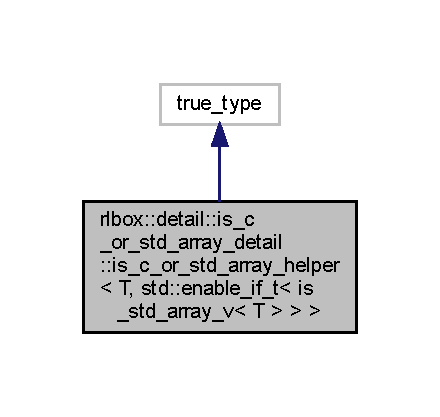
\includegraphics[width=223pt]{structrlbox_1_1detail_1_1is__c__or__std__array__detail_1_1is__c__or__std__array__helper_3_01T_00c572c4621f526c0df5dd6d2916a8cafa}
\end{center}
\end{figure}


Collaboration diagram for rlbox\+::detail\+::is\+\_\+c\+\_\+or\+\_\+std\+\_\+array\+\_\+detail\+::is\+\_\+c\+\_\+or\+\_\+std\+\_\+array\+\_\+helper$<$ T, std\+::enable\+\_\+if\+\_\+t$<$ is\+\_\+std\+\_\+array\+\_\+v$<$ T $>$ $>$ $>$\+:
\nopagebreak
\begin{figure}[H]
\begin{center}
\leavevmode
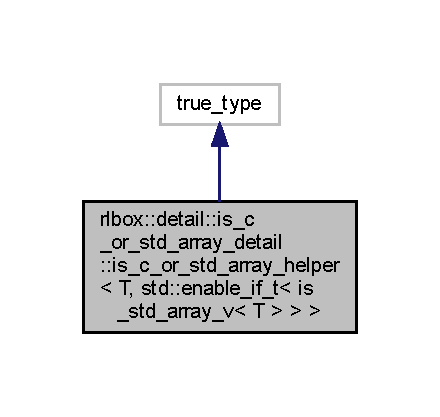
\includegraphics[width=223pt]{structrlbox_1_1detail_1_1is__c__or__std__array__detail_1_1is__c__or__std__array__helper_3_01T_00b9bd08b17ada9e028b847337d10afa56}
\end{center}
\end{figure}


The documentation for this struct was generated from the following file\+:\begin{DoxyCompactItemize}
\item 
/home/d/hack/rlbox\+\_\+sandboxing\+\_\+api/code/include/rlbox\+\_\+type\+\_\+traits.\+hpp\end{DoxyCompactItemize}

\hypertarget{structrlbox_1_1detail_1_1is__c__or__std__array__detail_1_1is__c__or__std__array__helper_3_01T_00e23e81f699b5338ffda7a4814dc1a20e}{}\doxysection{rlbox\+::detail\+::is\+\_\+c\+\_\+or\+\_\+std\+\_\+array\+\_\+detail\+::is\+\_\+c\+\_\+or\+\_\+std\+\_\+array\+\_\+helper$<$ T, std\+::enable\+\_\+if\+\_\+t$<$ std\+::is\+\_\+array\+\_\+v$<$ T $>$ $>$ $>$ Struct Template Reference}
\label{structrlbox_1_1detail_1_1is__c__or__std__array__detail_1_1is__c__or__std__array__helper_3_01T_00e23e81f699b5338ffda7a4814dc1a20e}\index{rlbox::detail::is\_c\_or\_std\_array\_detail::is\_c\_or\_std\_array\_helper$<$ T, std::enable\_if\_t$<$ std::is\_array\_v$<$ T $>$ $>$ $>$@{rlbox::detail::is\_c\_or\_std\_array\_detail::is\_c\_or\_std\_array\_helper$<$ T, std::enable\_if\_t$<$ std::is\_array\_v$<$ T $>$ $>$ $>$}}


Inheritance diagram for rlbox\+::detail\+::is\+\_\+c\+\_\+or\+\_\+std\+\_\+array\+\_\+detail\+::is\+\_\+c\+\_\+or\+\_\+std\+\_\+array\+\_\+helper$<$ T, std\+::enable\+\_\+if\+\_\+t$<$ std\+::is\+\_\+array\+\_\+v$<$ T $>$ $>$ $>$\+:
\nopagebreak
\begin{figure}[H]
\begin{center}
\leavevmode
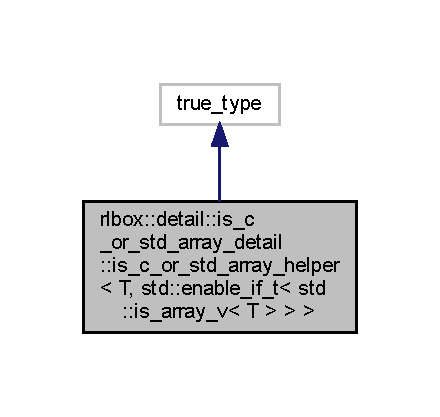
\includegraphics[width=211pt]{structrlbox_1_1detail_1_1is__c__or__std__array__detail_1_1is__c__or__std__array__helper_3_01T_005cef22c49da01f4aae103214978b4e9e}
\end{center}
\end{figure}


Collaboration diagram for rlbox\+::detail\+::is\+\_\+c\+\_\+or\+\_\+std\+\_\+array\+\_\+detail\+::is\+\_\+c\+\_\+or\+\_\+std\+\_\+array\+\_\+helper$<$ T, std\+::enable\+\_\+if\+\_\+t$<$ std\+::is\+\_\+array\+\_\+v$<$ T $>$ $>$ $>$\+:
\nopagebreak
\begin{figure}[H]
\begin{center}
\leavevmode
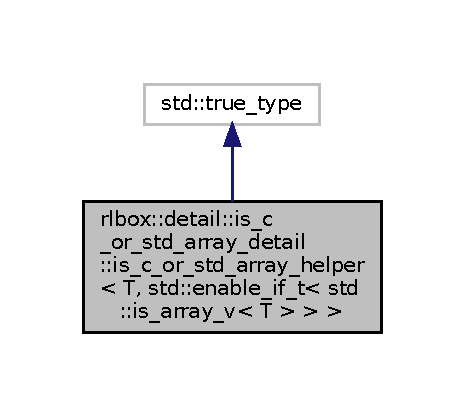
\includegraphics[width=211pt]{structrlbox_1_1detail_1_1is__c__or__std__array__detail_1_1is__c__or__std__array__helper_3_01T_00e165179d6402fff81dafd61404964f06}
\end{center}
\end{figure}


The documentation for this struct was generated from the following file\+:\begin{DoxyCompactItemize}
\item 
/home/shr/\+Code/\+Library\+Sandboxing/rlbox\+\_\+api\+\_\+cpp17/code/include/rlbox\+\_\+type\+\_\+traits.\+hpp\end{DoxyCompactItemize}

\hypertarget{structrlbox_1_1detail_1_1is__c__or__std__array__detail_1_1is__c__or__std__array__helper_3_01T_006917f5978f5075d5dadfc94abedf439f}{}\section{rlbox\+:\+:detail\+:\+:is\+\_\+c\+\_\+or\+\_\+std\+\_\+array\+\_\+detail\+:\+:is\+\_\+c\+\_\+or\+\_\+std\+\_\+array\+\_\+helper$<$ T, std\+:\+:enable\+\_\+if\+\_\+t$<$!std\+:\+:is\+\_\+array\+\_\+v$<$ T $>$ \&\&!is\+\_\+std\+\_\+array\+\_\+v$<$ T $>$ $>$ $>$ Struct Template Reference}
\label{structrlbox_1_1detail_1_1is__c__or__std__array__detail_1_1is__c__or__std__array__helper_3_01T_006917f5978f5075d5dadfc94abedf439f}\index{rlbox\+::detail\+::is\+\_\+c\+\_\+or\+\_\+std\+\_\+array\+\_\+detail\+::is\+\_\+c\+\_\+or\+\_\+std\+\_\+array\+\_\+helper$<$ T, std\+::enable\+\_\+if\+\_\+t$<$"!std\+::is\+\_\+array\+\_\+v$<$ T $>$ \&\&"!is\+\_\+std\+\_\+array\+\_\+v$<$ T $>$ $>$ $>$@{rlbox\+::detail\+::is\+\_\+c\+\_\+or\+\_\+std\+\_\+array\+\_\+detail\+::is\+\_\+c\+\_\+or\+\_\+std\+\_\+array\+\_\+helper$<$ T, std\+::enable\+\_\+if\+\_\+t$<$"!std\+::is\+\_\+array\+\_\+v$<$ T $>$ \&\&"!is\+\_\+std\+\_\+array\+\_\+v$<$ T $>$ $>$ $>$}}


Inheritance diagram for rlbox\+:\+:detail\+:\+:is\+\_\+c\+\_\+or\+\_\+std\+\_\+array\+\_\+detail\+:\+:is\+\_\+c\+\_\+or\+\_\+std\+\_\+array\+\_\+helper$<$ T, std\+:\+:enable\+\_\+if\+\_\+t$<$!std\+:\+:is\+\_\+array\+\_\+v$<$ T $>$ \&\&!is\+\_\+std\+\_\+array\+\_\+v$<$ T $>$ $>$ $>$\+:
\nopagebreak
\begin{figure}[H]
\begin{center}
\leavevmode
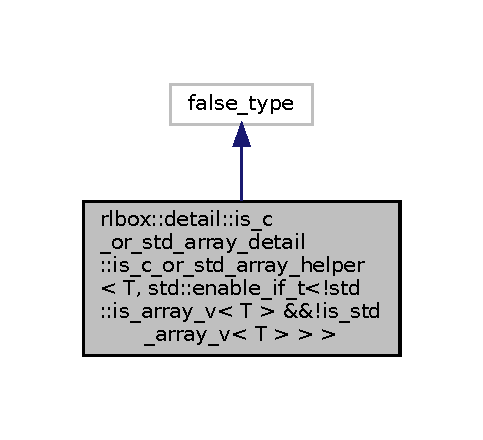
\includegraphics[width=217pt]{structrlbox_1_1detail_1_1is__c__or__std__array__detail_1_1is__c__or__std__array__helper_3_01T_0015ef7885df245dfa5b578f08ccc11aa3}
\end{center}
\end{figure}


Collaboration diagram for rlbox\+:\+:detail\+:\+:is\+\_\+c\+\_\+or\+\_\+std\+\_\+array\+\_\+detail\+:\+:is\+\_\+c\+\_\+or\+\_\+std\+\_\+array\+\_\+helper$<$ T, std\+:\+:enable\+\_\+if\+\_\+t$<$!std\+:\+:is\+\_\+array\+\_\+v$<$ T $>$ \&\&!is\+\_\+std\+\_\+array\+\_\+v$<$ T $>$ $>$ $>$\+:
\nopagebreak
\begin{figure}[H]
\begin{center}
\leavevmode
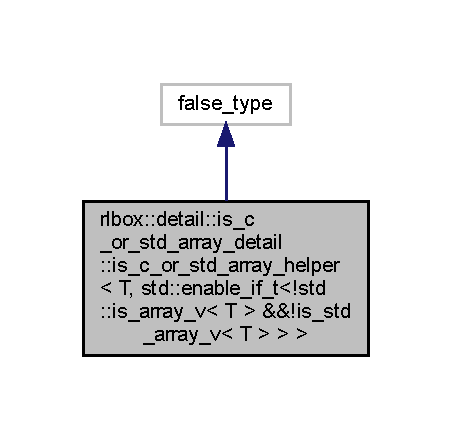
\includegraphics[width=217pt]{structrlbox_1_1detail_1_1is__c__or__std__array__detail_1_1is__c__or__std__array__helper_3_01T_00288e3a130f4a589742c8547d36cafb67}
\end{center}
\end{figure}


The documentation for this struct was generated from the following file\+:\begin{DoxyCompactItemize}
\item 
/home/shr/\+Code/\+Library\+Sandboxing/rlbox\+\_\+api\+\_\+cpp17/code/include/rlbox\+\_\+type\+\_\+traits.\+hpp\end{DoxyCompactItemize}

\hypertarget{structrlbox_1_1detail_1_1detail__is__member__of__rlbox__detail_1_1is__member__of__rlbox__detail__helper}{}\section{rlbox\+:\+:detail\+:\+:detail\+\_\+is\+\_\+member\+\_\+of\+\_\+rlbox\+\_\+detail\+:\+:is\+\_\+member\+\_\+of\+\_\+rlbox\+\_\+detail\+\_\+helper$<$ T, typename $>$ Struct Template Reference}
\label{structrlbox_1_1detail_1_1detail__is__member__of__rlbox__detail_1_1is__member__of__rlbox__detail__helper}\index{rlbox\+::detail\+::detail\+\_\+is\+\_\+member\+\_\+of\+\_\+rlbox\+\_\+detail\+::is\+\_\+member\+\_\+of\+\_\+rlbox\+\_\+detail\+\_\+helper$<$ T, typename $>$@{rlbox\+::detail\+::detail\+\_\+is\+\_\+member\+\_\+of\+\_\+rlbox\+\_\+detail\+::is\+\_\+member\+\_\+of\+\_\+rlbox\+\_\+detail\+\_\+helper$<$ T, typename $>$}}


Inheritance diagram for rlbox\+:\+:detail\+:\+:detail\+\_\+is\+\_\+member\+\_\+of\+\_\+rlbox\+\_\+detail\+:\+:is\+\_\+member\+\_\+of\+\_\+rlbox\+\_\+detail\+\_\+helper$<$ T, typename $>$\+:\nopagebreak
\begin{figure}[H]
\begin{center}
\leavevmode
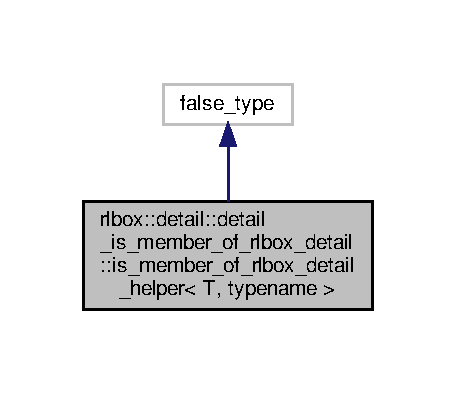
\includegraphics[width=235pt]{structrlbox_1_1detail_1_1detail__is__member__of__rlbox__detail_1_1is__member__of__rlbox__detail__helper__inherit__graph}
\end{center}
\end{figure}


Collaboration diagram for rlbox\+:\+:detail\+:\+:detail\+\_\+is\+\_\+member\+\_\+of\+\_\+rlbox\+\_\+detail\+:\+:is\+\_\+member\+\_\+of\+\_\+rlbox\+\_\+detail\+\_\+helper$<$ T, typename $>$\+:\nopagebreak
\begin{figure}[H]
\begin{center}
\leavevmode
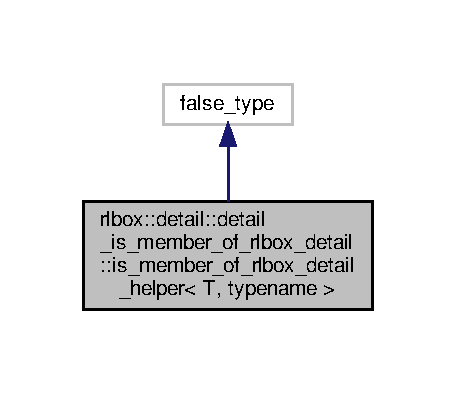
\includegraphics[width=235pt]{structrlbox_1_1detail_1_1detail__is__member__of__rlbox__detail_1_1is__member__of__rlbox__detail__helper__coll__graph}
\end{center}
\end{figure}


The documentation for this struct was generated from the following file\+:\begin{DoxyCompactItemize}
\item 
/home/shr/\+Code/\+Library\+Sandboxing/rlbox\+\_\+api\+\_\+cpp17/code/include/rlbox\+\_\+wrapper\+\_\+traits.\+hpp\end{DoxyCompactItemize}

\hypertarget{structrlbox_1_1detail_1_1detail__is__member__of__rlbox__detail_1_1is__member__of__rlbox__detail_586dbac5071c7fb9e9b52cfd4627c31a}{}\doxysection{rlbox\+::detail\+::detail\+\_\+is\+\_\+member\+\_\+of\+\_\+rlbox\+\_\+detail\+::is\+\_\+member\+\_\+of\+\_\+rlbox\+\_\+detail\+\_\+helper$<$ T, decltype(struct\+\_\+is\+\_\+member\+\_\+of\+\_\+rlbox\+\_\+detail(std\+::declval$<$ T $>$()))$>$ Struct Template Reference}
\label{structrlbox_1_1detail_1_1detail__is__member__of__rlbox__detail_1_1is__member__of__rlbox__detail_586dbac5071c7fb9e9b52cfd4627c31a}\index{rlbox::detail::detail\_is\_member\_of\_rlbox\_detail::is\_member\_of\_rlbox\_detail\_helper$<$ T, decltype(struct\_is\_member\_of\_rlbox\_detail(std::declval$<$ T $>$()))$>$@{rlbox::detail::detail\_is\_member\_of\_rlbox\_detail::is\_member\_of\_rlbox\_detail\_helper$<$ T, decltype(struct\_is\_member\_of\_rlbox\_detail(std::declval$<$ T $>$()))$>$}}


Inheritance diagram for rlbox\+::detail\+::detail\+\_\+is\+\_\+member\+\_\+of\+\_\+rlbox\+\_\+detail\+::is\+\_\+member\+\_\+of\+\_\+rlbox\+\_\+detail\+\_\+helper$<$ T, decltype(struct\+\_\+is\+\_\+member\+\_\+of\+\_\+rlbox\+\_\+detail(std\+::declval$<$ T $>$()))$>$\+:
\nopagebreak
\begin{figure}[H]
\begin{center}
\leavevmode
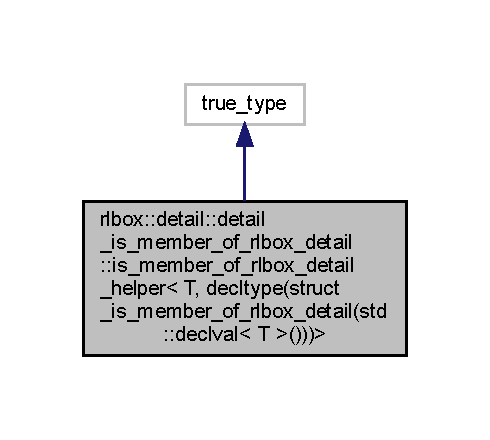
\includegraphics[width=235pt]{structrlbox_1_1detail_1_1detail__is__member__of__rlbox__detail_1_1is__member__of__rlbox__detail_2338b424c73790b40d6edf8f11a55113}
\end{center}
\end{figure}


Collaboration diagram for rlbox\+::detail\+::detail\+\_\+is\+\_\+member\+\_\+of\+\_\+rlbox\+\_\+detail\+::is\+\_\+member\+\_\+of\+\_\+rlbox\+\_\+detail\+\_\+helper$<$ T, decltype(struct\+\_\+is\+\_\+member\+\_\+of\+\_\+rlbox\+\_\+detail(std\+::declval$<$ T $>$()))$>$\+:
\nopagebreak
\begin{figure}[H]
\begin{center}
\leavevmode
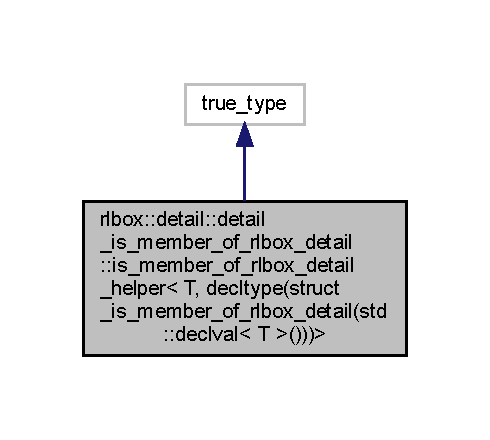
\includegraphics[width=235pt]{structrlbox_1_1detail_1_1detail__is__member__of__rlbox__detail_1_1is__member__of__rlbox__detail_338d0c4a83c58365a9c650d6cbd26600}
\end{center}
\end{figure}


The documentation for this struct was generated from the following file\+:\begin{DoxyCompactItemize}
\item 
/home/shr/\+Code/\+Library\+Sandboxing/rlbox\+\_\+api\+\_\+cpp17/code/include/rlbox\+\_\+wrapper\+\_\+traits.\+hpp\end{DoxyCompactItemize}

\hypertarget{structrlbox_1_1detail_1_1compile__time__for__detail_1_1num}{}\doxysection{rlbox\+::detail\+::compile\+\_\+time\+\_\+for\+\_\+detail\+::num$<$ N $>$ Struct Template Reference}
\label{structrlbox_1_1detail_1_1compile__time__for__detail_1_1num}\index{rlbox::detail::compile\_time\_for\_detail::num$<$ N $>$@{rlbox::detail::compile\_time\_for\_detail::num$<$ N $>$}}
\doxysubsection*{Static Public Attributes}
\begin{DoxyCompactItemize}
\item 
\mbox{\Hypertarget{structrlbox_1_1detail_1_1compile__time__for__detail_1_1num_a3ebecc6d20c6b147ad13c12b152999a7}\label{structrlbox_1_1detail_1_1compile__time__for__detail_1_1num_a3ebecc6d20c6b147ad13c12b152999a7}} 
static const constexpr auto {\bfseries value} = N
\end{DoxyCompactItemize}


The documentation for this struct was generated from the following file\+:\begin{DoxyCompactItemize}
\item 
/home/shr/\+Code/\+Library\+Sandboxing/rlbox\+\_\+api\+\_\+cpp17/code/include/rlbox\+\_\+helpers.\+hpp\end{DoxyCompactItemize}

\hypertarget{structrlbox_1_1detail_1_1remove__all__pointers__detail_1_1remove__all__pointers}{}\doxysection{rlbox\+::detail\+::remove\+\_\+all\+\_\+pointers\+\_\+detail\+::remove\+\_\+all\+\_\+pointers$<$ T $>$ Struct Template Reference}
\label{structrlbox_1_1detail_1_1remove__all__pointers__detail_1_1remove__all__pointers}\index{rlbox::detail::remove\_all\_pointers\_detail::remove\_all\_pointers$<$ T $>$@{rlbox::detail::remove\_all\_pointers\_detail::remove\_all\_pointers$<$ T $>$}}
\doxysubsection*{Public Types}
\begin{DoxyCompactItemize}
\item 
\mbox{\Hypertarget{structrlbox_1_1detail_1_1remove__all__pointers__detail_1_1remove__all__pointers_a663cf46e4718616fdf4d4a03e01d156e}\label{structrlbox_1_1detail_1_1remove__all__pointers__detail_1_1remove__all__pointers_a663cf46e4718616fdf4d4a03e01d156e}} 
typedef T {\bfseries type}
\end{DoxyCompactItemize}


The documentation for this struct was generated from the following file\+:\begin{DoxyCompactItemize}
\item 
/home/d/hack/rlbox\+\_\+sandboxing\+\_\+api/code/include/rlbox\+\_\+type\+\_\+traits.\+hpp\end{DoxyCompactItemize}

\hypertarget{structrlbox_1_1detail_1_1remove__all__pointers__detail_1_1remove__all__pointers_3_01T_01_5_01_4}{}\section{rlbox\+:\+:detail\+:\+:remove\+\_\+all\+\_\+pointers\+\_\+detail\+:\+:remove\+\_\+all\+\_\+pointers$<$ T $\ast$ $>$ Struct Template Reference}
\label{structrlbox_1_1detail_1_1remove__all__pointers__detail_1_1remove__all__pointers_3_01T_01_5_01_4}\index{rlbox\+::detail\+::remove\+\_\+all\+\_\+pointers\+\_\+detail\+::remove\+\_\+all\+\_\+pointers$<$ T $\ast$ $>$@{rlbox\+::detail\+::remove\+\_\+all\+\_\+pointers\+\_\+detail\+::remove\+\_\+all\+\_\+pointers$<$ T $\ast$ $>$}}
\subsection*{Public Types}
\begin{DoxyCompactItemize}
\item 
\mbox{\Hypertarget{structrlbox_1_1detail_1_1remove__all__pointers__detail_1_1remove__all__pointers_3_01T_01_5_01_4_a5e84dc13820435940c4f62c8b727be25}\label{structrlbox_1_1detail_1_1remove__all__pointers__detail_1_1remove__all__pointers_3_01T_01_5_01_4_a5e84dc13820435940c4f62c8b727be25}} 
typedef \hyperlink{structrlbox_1_1detail_1_1remove__all__pointers__detail_1_1remove__all__pointers}{remove\+\_\+all\+\_\+pointers}$<$ T $>$\+::type {\bfseries type}
\end{DoxyCompactItemize}


The documentation for this struct was generated from the following file\+:\begin{DoxyCompactItemize}
\item 
/home/shr/\+Code/\+Library\+Sandboxing/rlbox\+\_\+api\+\_\+cpp17/code/include/rlbox\+\_\+type\+\_\+traits.\+hpp\end{DoxyCompactItemize}

\hypertarget{classrlbox_1_1rlbox__noop__sandbox}{}\section{rlbox\+:\+:rlbox\+\_\+noop\+\_\+sandbox Class Reference}
\label{classrlbox_1_1rlbox__noop__sandbox}\index{rlbox\+::rlbox\+\_\+noop\+\_\+sandbox@{rlbox\+::rlbox\+\_\+noop\+\_\+sandbox}}


Class that implements the null sandbox. This sandbox doesn\textquotesingle{}t actually provide any isolation and only serves as a stepping stone towards migrating an application to use the R\+L\+Box A\+PI.  




{\ttfamily \#include $<$rlbox\+\_\+noop\+\_\+sandbox.\+hpp$>$}

\subsection*{Public Types}
\begin{DoxyCompactItemize}
\item 
\mbox{\Hypertarget{classrlbox_1_1rlbox__noop__sandbox_a54dfd9239da9ce4bdc48486ce03dfff6}\label{classrlbox_1_1rlbox__noop__sandbox_a54dfd9239da9ce4bdc48486ce03dfff6}} 
using {\bfseries T\+\_\+\+Long\+Long\+Type} = long long
\item 
\mbox{\Hypertarget{classrlbox_1_1rlbox__noop__sandbox_a6510f0a0d24a8af6f8b1ff759f9c27b1}\label{classrlbox_1_1rlbox__noop__sandbox_a6510f0a0d24a8af6f8b1ff759f9c27b1}} 
using {\bfseries T\+\_\+\+Long\+Type} = long
\item 
\mbox{\Hypertarget{classrlbox_1_1rlbox__noop__sandbox_aad50443cb7733460ca536ffd553aad08}\label{classrlbox_1_1rlbox__noop__sandbox_aad50443cb7733460ca536ffd553aad08}} 
using {\bfseries T\+\_\+\+Int\+Type} = int
\item 
\mbox{\Hypertarget{classrlbox_1_1rlbox__noop__sandbox_a909dbb8c3226fbcd19171c0548f21acf}\label{classrlbox_1_1rlbox__noop__sandbox_a909dbb8c3226fbcd19171c0548f21acf}} 
using {\bfseries T\+\_\+\+Pointer\+Type} = uintptr\+\_\+t
\item 
\mbox{\Hypertarget{classrlbox_1_1rlbox__noop__sandbox_a0bacaced018f138bf097b8e854c3ad5f}\label{classrlbox_1_1rlbox__noop__sandbox_a0bacaced018f138bf097b8e854c3ad5f}} 
using {\bfseries T\+\_\+\+Short\+Type} = short
\end{DoxyCompactItemize}
\subsection*{Protected Member Functions}
\begin{DoxyCompactItemize}
\item 
\mbox{\Hypertarget{classrlbox_1_1rlbox__noop__sandbox_aed3d297784c5654e6d83d4c5d3dacd90}\label{classrlbox_1_1rlbox__noop__sandbox_aed3d297784c5654e6d83d4c5d3dacd90}} 
void {\bfseries impl\+\_\+create\+\_\+sandbox} ()
\item 
\mbox{\Hypertarget{classrlbox_1_1rlbox__noop__sandbox_af1693fb4ff2ac776671d10c2c5481d61}\label{classrlbox_1_1rlbox__noop__sandbox_af1693fb4ff2ac776671d10c2c5481d61}} 
void {\bfseries impl\+\_\+destroy\+\_\+sandbox} ()
\item 
\mbox{\Hypertarget{classrlbox_1_1rlbox__noop__sandbox_aba431d23d82710301c8c1fe0b7cbf780}\label{classrlbox_1_1rlbox__noop__sandbox_aba431d23d82710301c8c1fe0b7cbf780}} 
{\footnotesize template$<$typename T $>$ }\\void $\ast$ {\bfseries impl\+\_\+get\+\_\+unsandboxed\+\_\+pointer} (T\+\_\+\+Pointer\+Type p) const
\item 
\mbox{\Hypertarget{classrlbox_1_1rlbox__noop__sandbox_acc83ff58dfef4a5a9c79a0e5b46fbec7}\label{classrlbox_1_1rlbox__noop__sandbox_acc83ff58dfef4a5a9c79a0e5b46fbec7}} 
{\footnotesize template$<$typename T $>$ }\\T\+\_\+\+Pointer\+Type {\bfseries impl\+\_\+get\+\_\+sandboxed\+\_\+pointer} (const void $\ast$p) const
\item 
\mbox{\Hypertarget{classrlbox_1_1rlbox__noop__sandbox_ada393a58fd84c379715f1361df3a1c5d}\label{classrlbox_1_1rlbox__noop__sandbox_ada393a58fd84c379715f1361df3a1c5d}} 
T\+\_\+\+Pointer\+Type {\bfseries impl\+\_\+malloc\+\_\+in\+\_\+sandbox} (size\+\_\+t size)
\item 
\mbox{\Hypertarget{classrlbox_1_1rlbox__noop__sandbox_a8722d866e0ebf476050dfa31cc30c2c4}\label{classrlbox_1_1rlbox__noop__sandbox_a8722d866e0ebf476050dfa31cc30c2c4}} 
void {\bfseries impl\+\_\+free\+\_\+in\+\_\+sandbox} (T\+\_\+\+Pointer\+Type p)
\item 
\mbox{\Hypertarget{classrlbox_1_1rlbox__noop__sandbox_ac2eacc65e2a7ab0ca01e1f9ba489422b}\label{classrlbox_1_1rlbox__noop__sandbox_ac2eacc65e2a7ab0ca01e1f9ba489422b}} 
bool {\bfseries impl\+\_\+is\+\_\+pointer\+\_\+in\+\_\+sandbox\+\_\+memory} (const void $\ast$)
\item 
\mbox{\Hypertarget{classrlbox_1_1rlbox__noop__sandbox_a9c1e09e364ee2a9b0e4661664dfd0892}\label{classrlbox_1_1rlbox__noop__sandbox_a9c1e09e364ee2a9b0e4661664dfd0892}} 
bool {\bfseries impl\+\_\+is\+\_\+pointer\+\_\+in\+\_\+app\+\_\+memory} (const void $\ast$)
\item 
\mbox{\Hypertarget{classrlbox_1_1rlbox__noop__sandbox_a5b0f5a989ec5b17cfe32ed469231ea16}\label{classrlbox_1_1rlbox__noop__sandbox_a5b0f5a989ec5b17cfe32ed469231ea16}} 
size\+\_\+t {\bfseries impl\+\_\+get\+\_\+total\+\_\+memory} ()
\item 
\mbox{\Hypertarget{classrlbox_1_1rlbox__noop__sandbox_ace3002edfb4b3758ab62d18f2388c491}\label{classrlbox_1_1rlbox__noop__sandbox_ace3002edfb4b3758ab62d18f2388c491}} 
void $\ast$ {\bfseries impl\+\_\+get\+\_\+memory\+\_\+location} ()
\item 
\mbox{\Hypertarget{classrlbox_1_1rlbox__noop__sandbox_acdf126ad5afb5dc94686bda3e9b1a36f}\label{classrlbox_1_1rlbox__noop__sandbox_acdf126ad5afb5dc94686bda3e9b1a36f}} 
{\footnotesize template$<$typename T  = void$>$ }\\void $\ast$ {\bfseries impl\+\_\+lookup\+\_\+symbol} (const char $\ast$)
\item 
\mbox{\Hypertarget{classrlbox_1_1rlbox__noop__sandbox_a0833932a29d618a1ab9d047e4a215657}\label{classrlbox_1_1rlbox__noop__sandbox_a0833932a29d618a1ab9d047e4a215657}} 
{\footnotesize template$<$typename T , typename T\+\_\+\+Converted , typename... T\+\_\+\+Args$>$ }\\auto {\bfseries impl\+\_\+invoke\+\_\+with\+\_\+func\+\_\+ptr} (T\+\_\+\+Converted $\ast$func\+\_\+ptr, T\+\_\+\+Args \&\&... params)
\item 
\mbox{\Hypertarget{classrlbox_1_1rlbox__noop__sandbox_ae787e181a8d293b115c0890e8036f03e}\label{classrlbox_1_1rlbox__noop__sandbox_ae787e181a8d293b115c0890e8036f03e}} 
{\footnotesize template$<$typename T\+\_\+\+Ret , typename... T\+\_\+\+Args$>$ }\\T\+\_\+\+Pointer\+Type {\bfseries impl\+\_\+register\+\_\+callback} (void $\ast$key, void $\ast$callback)
\item 
\mbox{\Hypertarget{classrlbox_1_1rlbox__noop__sandbox_a2949f30bdc7cdc297042465818357ca0}\label{classrlbox_1_1rlbox__noop__sandbox_a2949f30bdc7cdc297042465818357ca0}} 
{\footnotesize template$<$typename T\+\_\+\+Ret , typename... T\+\_\+\+Args$>$ }\\void {\bfseries impl\+\_\+unregister\+\_\+callback} (void $\ast$key)
\end{DoxyCompactItemize}
\subsection*{Static Protected Member Functions}
\begin{DoxyCompactItemize}
\item 
\mbox{\Hypertarget{classrlbox_1_1rlbox__noop__sandbox_ad8e4d197b5da2ed5028b96ebe03c81dd}\label{classrlbox_1_1rlbox__noop__sandbox_ad8e4d197b5da2ed5028b96ebe03c81dd}} 
{\footnotesize template$<$typename T $>$ }\\static void $\ast$ {\bfseries impl\+\_\+get\+\_\+unsandboxed\+\_\+pointer\+\_\+no\+\_\+ctx} (T\+\_\+\+Pointer\+Type p, const void $\ast$, \hyperlink{classrlbox_1_1rlbox__noop__sandbox}{rlbox\+\_\+noop\+\_\+sandbox} $\ast$($\ast$)(const void $\ast$example\+\_\+unsandboxed\+\_\+ptr))
\item 
\mbox{\Hypertarget{classrlbox_1_1rlbox__noop__sandbox_a267c49ce62893a37fc138d7a26c30123}\label{classrlbox_1_1rlbox__noop__sandbox_a267c49ce62893a37fc138d7a26c30123}} 
{\footnotesize template$<$typename T $>$ }\\static T\+\_\+\+Pointer\+Type {\bfseries impl\+\_\+get\+\_\+sandboxed\+\_\+pointer\+\_\+no\+\_\+ctx} (const void $\ast$p, const void $\ast$, \hyperlink{classrlbox_1_1rlbox__noop__sandbox}{rlbox\+\_\+noop\+\_\+sandbox} $\ast$($\ast$)(const void $\ast$example\+\_\+unsandboxed\+\_\+ptr))
\item 
\mbox{\Hypertarget{classrlbox_1_1rlbox__noop__sandbox_a5f720e5813f800fe573b028ce363760a}\label{classrlbox_1_1rlbox__noop__sandbox_a5f720e5813f800fe573b028ce363760a}} 
static bool {\bfseries impl\+\_\+is\+\_\+in\+\_\+same\+\_\+sandbox} (const void $\ast$, const void $\ast$)
\item 
\mbox{\Hypertarget{classrlbox_1_1rlbox__noop__sandbox_a4166590503035668cd74a63755cd1167}\label{classrlbox_1_1rlbox__noop__sandbox_a4166590503035668cd74a63755cd1167}} 
static std\+::pair$<$ \hyperlink{classrlbox_1_1rlbox__noop__sandbox}{rlbox\+\_\+noop\+\_\+sandbox} $\ast$, void $\ast$ $>$ {\bfseries impl\+\_\+get\+\_\+executed\+\_\+callback\+\_\+sandbox\+\_\+and\+\_\+key} ()
\end{DoxyCompactItemize}


\subsection{Detailed Description}
Class that implements the null sandbox. This sandbox doesn\textquotesingle{}t actually provide any isolation and only serves as a stepping stone towards migrating an application to use the R\+L\+Box A\+PI. 

The documentation for this class was generated from the following file\+:\begin{DoxyCompactItemize}
\item 
/home/shr/\+Code/\+Library\+Sandboxing/rlbox\+\_\+api\+\_\+cpp17/code/include/rlbox\+\_\+noop\+\_\+sandbox.\+hpp\end{DoxyCompactItemize}

\hypertarget{classrlbox_1_1rlbox__sandbox}{}\doxysection{rlbox\+::rlbox\+\_\+sandbox$<$ T\+\_\+\+Sbx $>$ Class Template Reference}
\label{classrlbox_1_1rlbox__sandbox}\index{rlbox::rlbox\_sandbox$<$ T\_Sbx $>$@{rlbox::rlbox\_sandbox$<$ T\_Sbx $>$}}


Encapsulation for sandboxes.  




{\ttfamily \#include $<$rlbox\+\_\+sandbox.\+hpp$>$}



Inheritance diagram for rlbox\+::rlbox\+\_\+sandbox$<$ T\+\_\+\+Sbx $>$\+:\nopagebreak
\begin{figure}[H]
\begin{center}
\leavevmode
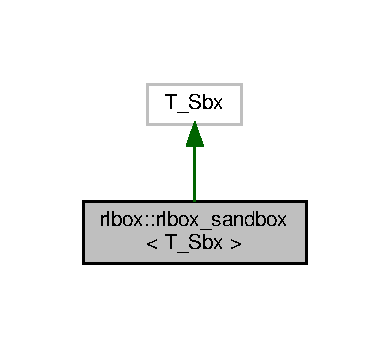
\includegraphics[width=187pt]{classrlbox_1_1rlbox__sandbox__inherit__graph}
\end{center}
\end{figure}


Collaboration diagram for rlbox\+::rlbox\+\_\+sandbox$<$ T\+\_\+\+Sbx $>$\+:\nopagebreak
\begin{figure}[H]
\begin{center}
\leavevmode
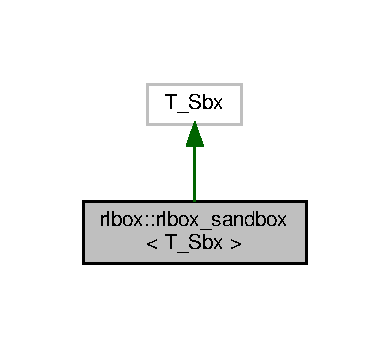
\includegraphics[width=187pt]{classrlbox_1_1rlbox__sandbox__coll__graph}
\end{center}
\end{figure}
\doxysubsection*{Public Types}
\begin{DoxyCompactItemize}
\item 
\mbox{\Hypertarget{classrlbox_1_1rlbox__sandbox_a2236c8f780e2fbb505b616a05d632298}\label{classrlbox_1_1rlbox__sandbox_a2236c8f780e2fbb505b616a05d632298}} 
{\footnotesize template$<$typename T $>$ }\\using {\bfseries convert\+\_\+to\+\_\+sandbox\+\_\+equivalent\+\_\+nonclass\+\_\+t} = detail\+::convert\+\_\+base\+\_\+types\+\_\+t$<$ T, typename T\+\_\+\+Sbx\+::\+T\+\_\+\+Short\+Type, typename T\+\_\+\+Sbx\+::\+T\+\_\+\+Int\+Type, typename T\+\_\+\+Sbx\+::\+T\+\_\+\+Long\+Type, typename T\+\_\+\+Sbx\+::\+T\+\_\+\+Long\+Long\+Type, typename T\+\_\+\+Sbx\+::\+T\+\_\+\+Pointer\+Type $>$
\item 
\mbox{\Hypertarget{classrlbox_1_1rlbox__sandbox_a09c972acd976ab264478c3abd32f8383}\label{classrlbox_1_1rlbox__sandbox_a09c972acd976ab264478c3abd32f8383}} 
{\footnotesize template$<$typename T\+\_\+\+Ret , typename... T\+\_\+\+Args$>$ }\\using {\bfseries T\+\_\+\+Cb\+\_\+no\+\_\+wrap} = detail\+::rlbox\+\_\+remove\+\_\+wrapper\+\_\+t$<$ T\+\_\+\+Ret $>$(detail\+::rlbox\+\_\+remove\+\_\+wrapper\+\_\+t$<$ T\+\_\+\+Args $>$...)
\end{DoxyCompactItemize}
\doxysubsection*{Public Member Functions}
\begin{DoxyCompactItemize}
\item 
\mbox{\Hypertarget{classrlbox_1_1rlbox__sandbox_a32de91755a582024dc43b879ef192b2c}\label{classrlbox_1_1rlbox__sandbox_a32de91755a582024dc43b879ef192b2c}} 
T\+\_\+\+Sbx $\ast$ {\bfseries get\+\_\+sandbox\+\_\+impl} ()
\item 
{\footnotesize template$<$typename... T\+\_\+\+Args$>$ }\\auto \mbox{\hyperlink{classrlbox_1_1rlbox__sandbox_a7b938866462f607bcc069770c1bc1ba6}{create\+\_\+sandbox}} (T\+\_\+\+Args... args)
\begin{DoxyCompactList}\small\item\em Create a new sandbox. \end{DoxyCompactList}\item 
\mbox{\Hypertarget{classrlbox_1_1rlbox__sandbox_ac2be161ed2183fa8bc319232a8d74da6}\label{classrlbox_1_1rlbox__sandbox_ac2be161ed2183fa8bc319232a8d74da6}} 
auto \mbox{\hyperlink{classrlbox_1_1rlbox__sandbox_ac2be161ed2183fa8bc319232a8d74da6}{destroy\+\_\+sandbox}} ()
\begin{DoxyCompactList}\small\item\em Destroy sandbox and reclaim any memory. \end{DoxyCompactList}\item 
\mbox{\Hypertarget{classrlbox_1_1rlbox__sandbox_a4776bcab38dc24395657d2c437e36fc8}\label{classrlbox_1_1rlbox__sandbox_a4776bcab38dc24395657d2c437e36fc8}} 
{\footnotesize template$<$typename T $>$ }\\T {\bfseries get\+\_\+unsandboxed\+\_\+pointer} (convert\+\_\+to\+\_\+sandbox\+\_\+equivalent\+\_\+nonclass\+\_\+t$<$ T $>$ p) const
\item 
\mbox{\Hypertarget{classrlbox_1_1rlbox__sandbox_aaef51e55536f08aa4c642f21d0de8008}\label{classrlbox_1_1rlbox__sandbox_aaef51e55536f08aa4c642f21d0de8008}} 
{\footnotesize template$<$typename T $>$ }\\convert\+\_\+to\+\_\+sandbox\+\_\+equivalent\+\_\+nonclass\+\_\+t$<$ T $>$ {\bfseries get\+\_\+sandboxed\+\_\+pointer} (const void $\ast$p) const
\item 
{\footnotesize template$<$typename T $>$ }\\\mbox{\hyperlink{classrlbox_1_1tainted}{tainted}}$<$ T $\ast$, T\+\_\+\+Sbx $>$ \mbox{\hyperlink{classrlbox_1_1rlbox__sandbox_ab6ecbc8d0d69a3305912fe92882ef6b9}{malloc\+\_\+in\+\_\+sandbox}} ()
\begin{DoxyCompactList}\small\item\em Allocate a new pointer that is accessible to both the application and sandbox. The pointer is allocated in sandbox memory. \end{DoxyCompactList}\item 
{\footnotesize template$<$typename T $>$ }\\\mbox{\hyperlink{classrlbox_1_1tainted}{tainted}}$<$ T $\ast$, T\+\_\+\+Sbx $>$ \mbox{\hyperlink{classrlbox_1_1rlbox__sandbox_a967ee4efa3c49a4493eaeda65b338e70}{malloc\+\_\+in\+\_\+sandbox}} (uint32\+\_\+t count)
\begin{DoxyCompactList}\small\item\em Allocate an array that is accessible to both the application and sandbox. The pointer is allocated in sandbox memory. \end{DoxyCompactList}\item 
{\footnotesize template$<$typename T $>$ }\\void \mbox{\hyperlink{classrlbox_1_1rlbox__sandbox_a775b1828f996dc8f14f24a296096e0e3}{free\+\_\+in\+\_\+sandbox}} (\mbox{\hyperlink{classrlbox_1_1tainted}{tainted}}$<$ T $\ast$, T\+\_\+\+Sbx $>$ ptr)
\begin{DoxyCompactList}\small\item\em Free the memory referenced by the tainted pointer. \end{DoxyCompactList}\item 
{\footnotesize template$<$typename T $>$ }\\void \mbox{\hyperlink{classrlbox_1_1rlbox__sandbox_ad26f351fa58e8fa013e79afb996dc807}{free\+\_\+in\+\_\+sandbox}} (\mbox{\hyperlink{classrlbox_1_1tainted__volatile}{tainted\+\_\+volatile}}$<$ T, T\+\_\+\+Sbx $>$ \&ptr\+\_\+ref)
\begin{DoxyCompactList}\small\item\em Free the memory referenced by a \mbox{\hyperlink{classrlbox_1_1tainted__volatile}{tainted\+\_\+volatile}} pointer ref. \end{DoxyCompactList}\item 
{\footnotesize template$<$typename T $>$ }\\void \mbox{\hyperlink{classrlbox_1_1rlbox__sandbox_a75636dbe30d516a71f13841a4a64a854}{free\+\_\+in\+\_\+sandbox}} (\mbox{\hyperlink{classrlbox_1_1tainted__opaque}{tainted\+\_\+opaque}}$<$ T, T\+\_\+\+Sbx $>$ ptr\+\_\+opaque)
\begin{DoxyCompactList}\small\item\em Free the memory referenced by a \mbox{\hyperlink{classrlbox_1_1tainted__opaque}{tainted\+\_\+opaque}} pointer. \end{DoxyCompactList}\item 
\mbox{\Hypertarget{classrlbox_1_1rlbox__sandbox_a55e48f0300c16d36ea7ed5a7e4750f64}\label{classrlbox_1_1rlbox__sandbox_a55e48f0300c16d36ea7ed5a7e4750f64}} 
bool \mbox{\hyperlink{classrlbox_1_1rlbox__sandbox_a55e48f0300c16d36ea7ed5a7e4750f64}{is\+\_\+pointer\+\_\+in\+\_\+sandbox\+\_\+memory}} (const void $\ast$p)
\begin{DoxyCompactList}\small\item\em Check if the pointer points to this sandbox\textquotesingle{}s memory. For the null-\/sandbox, this always returns true. \end{DoxyCompactList}\item 
\mbox{\Hypertarget{classrlbox_1_1rlbox__sandbox_afc6c3f229b2807517c54cc120dfda941}\label{classrlbox_1_1rlbox__sandbox_afc6c3f229b2807517c54cc120dfda941}} 
bool \mbox{\hyperlink{classrlbox_1_1rlbox__sandbox_afc6c3f229b2807517c54cc120dfda941}{is\+\_\+pointer\+\_\+in\+\_\+app\+\_\+memory}} (const void $\ast$p)
\begin{DoxyCompactList}\small\item\em Check if the pointer points to application memory. For the null-\/sandbox, this always returns true. \end{DoxyCompactList}\item 
\mbox{\Hypertarget{classrlbox_1_1rlbox__sandbox_a9bfda00c80c73e70ddbc3f2419066cb8}\label{classrlbox_1_1rlbox__sandbox_a9bfda00c80c73e70ddbc3f2419066cb8}} 
size\+\_\+t {\bfseries get\+\_\+total\+\_\+memory} ()
\item 
\mbox{\Hypertarget{classrlbox_1_1rlbox__sandbox_af682f225ef74ad07cfa5c25e7c8ed42c}\label{classrlbox_1_1rlbox__sandbox_af682f225ef74ad07cfa5c25e7c8ed42c}} 
void $\ast$ {\bfseries get\+\_\+memory\+\_\+location} ()
\item 
\mbox{\Hypertarget{classrlbox_1_1rlbox__sandbox_a9b25c4fe571fbebd287fd5fbd5a2e2c7}\label{classrlbox_1_1rlbox__sandbox_a9b25c4fe571fbebd287fd5fbd5a2e2c7}} 
void $\ast$ {\bfseries get\+\_\+transition\+\_\+state} ()
\item 
\mbox{\Hypertarget{classrlbox_1_1rlbox__sandbox_a96d6a841818c4342bb905670cfc3ca11}\label{classrlbox_1_1rlbox__sandbox_a96d6a841818c4342bb905670cfc3ca11}} 
void {\bfseries set\+\_\+transition\+\_\+state} (void $\ast$new\+\_\+state)
\item 
{\footnotesize template$<$typename T $>$ }\\\mbox{\hyperlink{classrlbox_1_1tainted}{tainted}}$<$ T $\ast$, T\+\_\+\+Sbx $>$ \mbox{\hyperlink{classrlbox_1_1rlbox__sandbox_ada1ed84dee64fc8fae57c38b36d77f02}{INTERNAL\+\_\+grant\+\_\+access}} (T $\ast$src, size\+\_\+t num, bool \&success)
\begin{DoxyCompactList}\small\item\em For internal use only. Grant access of the passed in buffer in to the sandbox instance. Called by internal APIs only if the underlying sandbox supports can\+\_\+grant\+\_\+deny\+\_\+access by including the line. \end{DoxyCompactList}\item 
{\footnotesize template$<$typename T $>$ }\\T $\ast$ \mbox{\hyperlink{classrlbox_1_1rlbox__sandbox_a559c3f9ba49a099f959a0bdc9e48090d}{INTERNAL\+\_\+deny\+\_\+access}} (\mbox{\hyperlink{classrlbox_1_1tainted}{tainted}}$<$ T $\ast$, T\+\_\+\+Sbx $>$ src, size\+\_\+t num, bool \&success)
\begin{DoxyCompactList}\small\item\em For internal use only. Grant access of the passed in buffer in to the sandbox instance. Called by internal APIs only if the underlying sandbox supports can\+\_\+grant\+\_\+deny\+\_\+access by including the line. \end{DoxyCompactList}\item 
\mbox{\Hypertarget{classrlbox_1_1rlbox__sandbox_a38b2f18b1db0dbd789477a93d0dc40eb}\label{classrlbox_1_1rlbox__sandbox_a38b2f18b1db0dbd789477a93d0dc40eb}} 
void $\ast$ {\bfseries lookup\+\_\+symbol} (const char $\ast$func\+\_\+name)
\item 
\mbox{\Hypertarget{classrlbox_1_1rlbox__sandbox_a9f9e13680f09205f25a520fc04ef3f9a}\label{classrlbox_1_1rlbox__sandbox_a9f9e13680f09205f25a520fc04ef3f9a}} 
{\footnotesize template$<$typename T , typename... T\+\_\+\+Args$>$ }\\auto {\bfseries INTERNAL\+\_\+invoke\+\_\+with\+\_\+func\+\_\+name} (const char $\ast$func\+\_\+name, T\+\_\+\+Args \&\&... params)
\item 
\mbox{\Hypertarget{classrlbox_1_1rlbox__sandbox_a5eacf092a66c9d4f850b726ffdcd9926}\label{classrlbox_1_1rlbox__sandbox_a5eacf092a66c9d4f850b726ffdcd9926}} 
{\footnotesize template$<$typename T , typename... T\+\_\+\+Args$>$ }\\auto {\bfseries INTERNAL\+\_\+invoke\+\_\+with\+\_\+func\+\_\+ptr} (const char $\ast$func\+\_\+name, void $\ast$func\+\_\+ptr, T\+\_\+\+Args \&\&... params)
\item 
\mbox{\Hypertarget{classrlbox_1_1rlbox__sandbox_acd10ff63b848c01690ba1f8977621a72}\label{classrlbox_1_1rlbox__sandbox_acd10ff63b848c01690ba1f8977621a72}} 
{\footnotesize template$<$typename T2 $>$ }\\\mbox{\hyperlink{classrlbox_1_1tainted}{tainted}}$<$ T2, T\+\_\+\+Sbx $>$ {\bfseries UNSAFE\+\_\+accept\+\_\+pointer} (T2 ptr)
\item 
\mbox{\Hypertarget{classrlbox_1_1rlbox__sandbox_ad2cf7d6b28eca1cdc04cb3cbee338189}\label{classrlbox_1_1rlbox__sandbox_ad2cf7d6b28eca1cdc04cb3cbee338189}} 
{\footnotesize template$<$typename T\+\_\+\+Ret $>$ }\\\mbox{\hyperlink{classrlbox_1_1sandbox__callback}{sandbox\+\_\+callback}}$<$ T\+\_\+\+Cb\+\_\+no\+\_\+wrap$<$ T\+\_\+\+Ret $>$ $\ast$, T\+\_\+\+Sbx $>$ {\bfseries register\+\_\+callback} (T\+\_\+\+Ret($\ast$)())
\item 
{\footnotesize template$<$typename T\+\_\+\+RL , typename T\+\_\+\+Ret , typename... T\+\_\+\+Args$>$ }\\\mbox{\hyperlink{classrlbox_1_1sandbox__callback}{sandbox\+\_\+callback}}$<$ T\+\_\+\+Cb\+\_\+no\+\_\+wrap$<$ T\+\_\+\+Ret, T\+\_\+\+Args... $>$ $\ast$, T\+\_\+\+Sbx $>$ \mbox{\hyperlink{classrlbox_1_1rlbox__sandbox_ae4f4cc7825bcb613ab5405e0f6cae7f3}{register\+\_\+callback}} (T\+\_\+\+Ret($\ast$func\+\_\+ptr)(T\+\_\+\+RL, T\+\_\+\+Args...))
\begin{DoxyCompactList}\small\item\em Expose a callback function to the sandboxed code. \end{DoxyCompactList}\item 
\mbox{\Hypertarget{classrlbox_1_1rlbox__sandbox_ad65b42ed5e903655cc23cc9e33672b16}\label{classrlbox_1_1rlbox__sandbox_ad65b42ed5e903655cc23cc9e33672b16}} 
{\footnotesize template$<$typename T $>$ }\\\mbox{\hyperlink{classrlbox_1_1tainted}{tainted}}$<$ T $\ast$, T\+\_\+\+Sbx $>$ {\bfseries INTERNAL\+\_\+get\+\_\+sandbox\+\_\+function\+\_\+name} (const char $\ast$func\+\_\+name)
\item 
\mbox{\Hypertarget{classrlbox_1_1rlbox__sandbox_a912906aabd93bf8358153b7a4c7e0adc}\label{classrlbox_1_1rlbox__sandbox_a912906aabd93bf8358153b7a4c7e0adc}} 
{\footnotesize template$<$typename T $>$ }\\\mbox{\hyperlink{classrlbox_1_1tainted}{tainted}}$<$ T $\ast$, T\+\_\+\+Sbx $>$ {\bfseries INTERNAL\+\_\+get\+\_\+sandbox\+\_\+function\+\_\+ptr} (void $\ast$func\+\_\+ptr)
\item 
{\footnotesize template$<$typename T $>$ }\\\mbox{\hyperlink{classrlbox_1_1app__pointer}{app\+\_\+pointer}}$<$ T $\ast$, T\+\_\+\+Sbx $>$ \mbox{\hyperlink{classrlbox_1_1rlbox__sandbox_acc0f5bdfa77546148ed15d06641659a5}{get\+\_\+app\+\_\+pointer}} (T $\ast$ptr)
\begin{DoxyCompactList}\small\item\em Create a \char`\"{}fake\char`\"{} pointer referring to a location in the application memory. \end{DoxyCompactList}\item 
{\footnotesize template$<$typename T $>$ }\\T $\ast$ \mbox{\hyperlink{classrlbox_1_1rlbox__sandbox_a2ed22fa984d2b3cba5352afbd4211bcd}{lookup\+\_\+app\+\_\+ptr}} (\mbox{\hyperlink{classrlbox_1_1tainted}{tainted}}$<$ T $\ast$, T\+\_\+\+Sbx $>$ tainted\+\_\+ptr)
\begin{DoxyCompactList}\small\item\em The mirror of get\+\_\+app\+\_\+pointer. Take a tainted pointer which is actually an \mbox{\hyperlink{classrlbox_1_1app__pointer}{app\+\_\+pointer}}, and get the application location being pointed to. \end{DoxyCompactList}\end{DoxyCompactItemize}
\doxysubsection*{Static Public Member Functions}
\begin{DoxyCompactItemize}
\item 
\mbox{\Hypertarget{classrlbox_1_1rlbox__sandbox_a030d5e296cdeb24cd4ca99a5cbe0ea39}\label{classrlbox_1_1rlbox__sandbox_a030d5e296cdeb24cd4ca99a5cbe0ea39}} 
{\footnotesize template$<$typename T $>$ }\\static T {\bfseries get\+\_\+unsandboxed\+\_\+pointer\+\_\+no\+\_\+ctx} (convert\+\_\+to\+\_\+sandbox\+\_\+equivalent\+\_\+nonclass\+\_\+t$<$ T $>$ p, const void $\ast$example\+\_\+unsandboxed\+\_\+ptr)
\item 
\mbox{\Hypertarget{classrlbox_1_1rlbox__sandbox_a37e1e1468b883faf8a878b3c0a221d39}\label{classrlbox_1_1rlbox__sandbox_a37e1e1468b883faf8a878b3c0a221d39}} 
{\footnotesize template$<$typename T $>$ }\\static convert\+\_\+to\+\_\+sandbox\+\_\+equivalent\+\_\+nonclass\+\_\+t$<$ T $>$ {\bfseries get\+\_\+sandboxed\+\_\+pointer\+\_\+no\+\_\+ctx} (const void $\ast$p, const void $\ast$example\+\_\+unsandboxed\+\_\+ptr)
\item 
\mbox{\Hypertarget{classrlbox_1_1rlbox__sandbox_a3257ffc0e7eb6022c05a049b8b36271f}\label{classrlbox_1_1rlbox__sandbox_a3257ffc0e7eb6022c05a049b8b36271f}} 
static bool \mbox{\hyperlink{classrlbox_1_1rlbox__sandbox_a3257ffc0e7eb6022c05a049b8b36271f}{is\+\_\+in\+\_\+same\+\_\+sandbox}} (const void $\ast$p1, const void $\ast$p2)
\begin{DoxyCompactList}\small\item\em Check if two pointers are in the same sandbox. For the null-\/sandbox, this always returns true. \end{DoxyCompactList}\end{DoxyCompactItemize}
\doxysubsection*{Public Attributes}
\begin{DoxyCompactItemize}
\item 
\mbox{\Hypertarget{classrlbox_1_1rlbox__sandbox_a61db4d3c217ee7acbc40e0bab23449e8}\label{classrlbox_1_1rlbox__sandbox_a61db4d3c217ee7acbc40e0bab23449e8}} 
void $\ast$ \mbox{\hyperlink{classrlbox_1_1rlbox__sandbox_a61db4d3c217ee7acbc40e0bab23449e8}{sandbox\+\_\+storage}}
\begin{DoxyCompactList}\small\item\em Unused member that allows the calling code to save data in a \char`\"{}per-\/sandbox\char`\"{} storage. This can be useful to save context which is used in callbacks. \end{DoxyCompactList}\end{DoxyCompactItemize}


\doxysubsection{Detailed Description}
\subsubsection*{template$<$typename T\+\_\+\+Sbx$>$\newline
class rlbox\+::rlbox\+\_\+sandbox$<$ T\+\_\+\+Sbx $>$}

Encapsulation for sandboxes. 


\begin{DoxyTemplParams}{Template Parameters}
{\em T\+\_\+\+Sbx} & Type of sandbox. For the null sandbox this is {\ttfamily \mbox{\hyperlink{classrlbox_1_1rlbox__noop__sandbox}{rlbox\+\_\+noop\+\_\+sandbox}}} \\
\hline
\end{DoxyTemplParams}


\doxysubsection{Member Function Documentation}
\mbox{\Hypertarget{classrlbox_1_1rlbox__sandbox_a7b938866462f607bcc069770c1bc1ba6}\label{classrlbox_1_1rlbox__sandbox_a7b938866462f607bcc069770c1bc1ba6}} 
\index{rlbox::rlbox\_sandbox$<$ T\_Sbx $>$@{rlbox::rlbox\_sandbox$<$ T\_Sbx $>$}!create\_sandbox@{create\_sandbox}}
\index{create\_sandbox@{create\_sandbox}!rlbox::rlbox\_sandbox$<$ T\_Sbx $>$@{rlbox::rlbox\_sandbox$<$ T\_Sbx $>$}}
\doxysubsubsection{\texorpdfstring{create\_sandbox()}{create\_sandbox()}}
{\footnotesize\ttfamily template$<$typename T\+\_\+\+Sbx $>$ \\
template$<$typename... T\+\_\+\+Args$>$ \\
auto \mbox{\hyperlink{classrlbox_1_1rlbox__sandbox}{rlbox\+::rlbox\+\_\+sandbox}}$<$ T\+\_\+\+Sbx $>$\+::create\+\_\+sandbox (\begin{DoxyParamCaption}\item[{T\+\_\+\+Args...}]{args }\end{DoxyParamCaption})\hspace{0.3cm}{\ttfamily [inline]}}



Create a new sandbox. 


\begin{DoxyTemplParams}{Template Parameters}
{\em T\+\_\+args} & Arguments passed to the underlying sandbox implementation. For the null sandbox, no arguments are necessary. \\
\hline
\end{DoxyTemplParams}
\mbox{\Hypertarget{classrlbox_1_1rlbox__sandbox_a775b1828f996dc8f14f24a296096e0e3}\label{classrlbox_1_1rlbox__sandbox_a775b1828f996dc8f14f24a296096e0e3}} 
\index{rlbox::rlbox\_sandbox$<$ T\_Sbx $>$@{rlbox::rlbox\_sandbox$<$ T\_Sbx $>$}!free\_in\_sandbox@{free\_in\_sandbox}}
\index{free\_in\_sandbox@{free\_in\_sandbox}!rlbox::rlbox\_sandbox$<$ T\_Sbx $>$@{rlbox::rlbox\_sandbox$<$ T\_Sbx $>$}}
\doxysubsubsection{\texorpdfstring{free\_in\_sandbox()}{free\_in\_sandbox()}\hspace{0.1cm}{\footnotesize\ttfamily [1/3]}}
{\footnotesize\ttfamily template$<$typename T\+\_\+\+Sbx $>$ \\
template$<$typename T $>$ \\
void \mbox{\hyperlink{classrlbox_1_1rlbox__sandbox}{rlbox\+::rlbox\+\_\+sandbox}}$<$ T\+\_\+\+Sbx $>$\+::free\+\_\+in\+\_\+sandbox (\begin{DoxyParamCaption}\item[{\mbox{\hyperlink{classrlbox_1_1tainted}{tainted}}$<$ T $\ast$, T\+\_\+\+Sbx $>$}]{ptr }\end{DoxyParamCaption})\hspace{0.3cm}{\ttfamily [inline]}}



Free the memory referenced by the tainted pointer. 


\begin{DoxyParams}{Parameters}
{\em ptr} & Pointer to sandbox memory to free. \\
\hline
\end{DoxyParams}
\mbox{\Hypertarget{classrlbox_1_1rlbox__sandbox_a75636dbe30d516a71f13841a4a64a854}\label{classrlbox_1_1rlbox__sandbox_a75636dbe30d516a71f13841a4a64a854}} 
\index{rlbox::rlbox\_sandbox$<$ T\_Sbx $>$@{rlbox::rlbox\_sandbox$<$ T\_Sbx $>$}!free\_in\_sandbox@{free\_in\_sandbox}}
\index{free\_in\_sandbox@{free\_in\_sandbox}!rlbox::rlbox\_sandbox$<$ T\_Sbx $>$@{rlbox::rlbox\_sandbox$<$ T\_Sbx $>$}}
\doxysubsubsection{\texorpdfstring{free\_in\_sandbox()}{free\_in\_sandbox()}\hspace{0.1cm}{\footnotesize\ttfamily [2/3]}}
{\footnotesize\ttfamily template$<$typename T\+\_\+\+Sbx $>$ \\
template$<$typename T $>$ \\
void \mbox{\hyperlink{classrlbox_1_1rlbox__sandbox}{rlbox\+::rlbox\+\_\+sandbox}}$<$ T\+\_\+\+Sbx $>$\+::free\+\_\+in\+\_\+sandbox (\begin{DoxyParamCaption}\item[{\mbox{\hyperlink{classrlbox_1_1tainted__opaque}{tainted\+\_\+opaque}}$<$ T, T\+\_\+\+Sbx $>$}]{ptr\+\_\+opaque }\end{DoxyParamCaption})\hspace{0.3cm}{\ttfamily [inline]}}



Free the memory referenced by a \mbox{\hyperlink{classrlbox_1_1tainted__opaque}{tainted\+\_\+opaque}} pointer. 


\begin{DoxyParams}{Parameters}
{\em ptr\+\_\+opaque} & Opaque pointer to sandbox memory to free. \\
\hline
\end{DoxyParams}
\mbox{\Hypertarget{classrlbox_1_1rlbox__sandbox_ad26f351fa58e8fa013e79afb996dc807}\label{classrlbox_1_1rlbox__sandbox_ad26f351fa58e8fa013e79afb996dc807}} 
\index{rlbox::rlbox\_sandbox$<$ T\_Sbx $>$@{rlbox::rlbox\_sandbox$<$ T\_Sbx $>$}!free\_in\_sandbox@{free\_in\_sandbox}}
\index{free\_in\_sandbox@{free\_in\_sandbox}!rlbox::rlbox\_sandbox$<$ T\_Sbx $>$@{rlbox::rlbox\_sandbox$<$ T\_Sbx $>$}}
\doxysubsubsection{\texorpdfstring{free\_in\_sandbox()}{free\_in\_sandbox()}\hspace{0.1cm}{\footnotesize\ttfamily [3/3]}}
{\footnotesize\ttfamily template$<$typename T\+\_\+\+Sbx $>$ \\
template$<$typename T $>$ \\
void \mbox{\hyperlink{classrlbox_1_1rlbox__sandbox}{rlbox\+::rlbox\+\_\+sandbox}}$<$ T\+\_\+\+Sbx $>$\+::free\+\_\+in\+\_\+sandbox (\begin{DoxyParamCaption}\item[{\mbox{\hyperlink{classrlbox_1_1tainted__volatile}{tainted\+\_\+volatile}}$<$ T, T\+\_\+\+Sbx $>$ \&}]{ptr\+\_\+ref }\end{DoxyParamCaption})\hspace{0.3cm}{\ttfamily [inline]}}



Free the memory referenced by a \mbox{\hyperlink{classrlbox_1_1tainted__volatile}{tainted\+\_\+volatile}} pointer ref. 


\begin{DoxyParams}{Parameters}
{\em ptr\+\_\+ref} & Pointer reference to sandbox memory to free. \\
\hline
\end{DoxyParams}
\mbox{\Hypertarget{classrlbox_1_1rlbox__sandbox_acc0f5bdfa77546148ed15d06641659a5}\label{classrlbox_1_1rlbox__sandbox_acc0f5bdfa77546148ed15d06641659a5}} 
\index{rlbox::rlbox\_sandbox$<$ T\_Sbx $>$@{rlbox::rlbox\_sandbox$<$ T\_Sbx $>$}!get\_app\_pointer@{get\_app\_pointer}}
\index{get\_app\_pointer@{get\_app\_pointer}!rlbox::rlbox\_sandbox$<$ T\_Sbx $>$@{rlbox::rlbox\_sandbox$<$ T\_Sbx $>$}}
\doxysubsubsection{\texorpdfstring{get\_app\_pointer()}{get\_app\_pointer()}}
{\footnotesize\ttfamily template$<$typename T\+\_\+\+Sbx $>$ \\
template$<$typename T $>$ \\
\mbox{\hyperlink{classrlbox_1_1app__pointer}{app\+\_\+pointer}}$<$T$\ast$, T\+\_\+\+Sbx$>$ \mbox{\hyperlink{classrlbox_1_1rlbox__sandbox}{rlbox\+::rlbox\+\_\+sandbox}}$<$ T\+\_\+\+Sbx $>$\+::get\+\_\+app\+\_\+pointer (\begin{DoxyParamCaption}\item[{T $\ast$}]{ptr }\end{DoxyParamCaption})\hspace{0.3cm}{\ttfamily [inline]}}



Create a \char`\"{}fake\char`\"{} pointer referring to a location in the application memory. 


\begin{DoxyParams}{Parameters}
{\em ptr} & The pointer to refer to\\
\hline
\end{DoxyParams}
\begin{DoxyReturn}{Returns}
The \mbox{\hyperlink{classrlbox_1_1app__pointer}{app\+\_\+pointer}} object that refers to this location. 
\end{DoxyReturn}
\mbox{\Hypertarget{classrlbox_1_1rlbox__sandbox_a559c3f9ba49a099f959a0bdc9e48090d}\label{classrlbox_1_1rlbox__sandbox_a559c3f9ba49a099f959a0bdc9e48090d}} 
\index{rlbox::rlbox\_sandbox$<$ T\_Sbx $>$@{rlbox::rlbox\_sandbox$<$ T\_Sbx $>$}!INTERNAL\_deny\_access@{INTERNAL\_deny\_access}}
\index{INTERNAL\_deny\_access@{INTERNAL\_deny\_access}!rlbox::rlbox\_sandbox$<$ T\_Sbx $>$@{rlbox::rlbox\_sandbox$<$ T\_Sbx $>$}}
\doxysubsubsection{\texorpdfstring{INTERNAL\_deny\_access()}{INTERNAL\_deny\_access()}}
{\footnotesize\ttfamily template$<$typename T\+\_\+\+Sbx $>$ \\
template$<$typename T $>$ \\
T$\ast$ \mbox{\hyperlink{classrlbox_1_1rlbox__sandbox}{rlbox\+::rlbox\+\_\+sandbox}}$<$ T\+\_\+\+Sbx $>$\+::INTERNAL\+\_\+deny\+\_\+access (\begin{DoxyParamCaption}\item[{\mbox{\hyperlink{classrlbox_1_1tainted}{tainted}}$<$ T $\ast$, T\+\_\+\+Sbx $>$}]{src,  }\item[{size\+\_\+t}]{num,  }\item[{bool \&}]{success }\end{DoxyParamCaption})\hspace{0.3cm}{\ttfamily [inline]}}



For internal use only. Grant access of the passed in buffer in to the sandbox instance. Called by internal APIs only if the underlying sandbox supports can\+\_\+grant\+\_\+deny\+\_\+access by including the line. 


\begin{DoxyCode}{0}
\DoxyCodeLine{\textcolor{keyword}{using} can\_grant\_deny\_access = void;}

\end{DoxyCode}
 \mbox{\Hypertarget{classrlbox_1_1rlbox__sandbox_ada1ed84dee64fc8fae57c38b36d77f02}\label{classrlbox_1_1rlbox__sandbox_ada1ed84dee64fc8fae57c38b36d77f02}} 
\index{rlbox::rlbox\_sandbox$<$ T\_Sbx $>$@{rlbox::rlbox\_sandbox$<$ T\_Sbx $>$}!INTERNAL\_grant\_access@{INTERNAL\_grant\_access}}
\index{INTERNAL\_grant\_access@{INTERNAL\_grant\_access}!rlbox::rlbox\_sandbox$<$ T\_Sbx $>$@{rlbox::rlbox\_sandbox$<$ T\_Sbx $>$}}
\doxysubsubsection{\texorpdfstring{INTERNAL\_grant\_access()}{INTERNAL\_grant\_access()}}
{\footnotesize\ttfamily template$<$typename T\+\_\+\+Sbx $>$ \\
template$<$typename T $>$ \\
\mbox{\hyperlink{classrlbox_1_1tainted}{tainted}}$<$T$\ast$, T\+\_\+\+Sbx$>$ \mbox{\hyperlink{classrlbox_1_1rlbox__sandbox}{rlbox\+::rlbox\+\_\+sandbox}}$<$ T\+\_\+\+Sbx $>$\+::INTERNAL\+\_\+grant\+\_\+access (\begin{DoxyParamCaption}\item[{T $\ast$}]{src,  }\item[{size\+\_\+t}]{num,  }\item[{bool \&}]{success }\end{DoxyParamCaption})\hspace{0.3cm}{\ttfamily [inline]}}



For internal use only. Grant access of the passed in buffer in to the sandbox instance. Called by internal APIs only if the underlying sandbox supports can\+\_\+grant\+\_\+deny\+\_\+access by including the line. 


\begin{DoxyCode}{0}
\DoxyCodeLine{\textcolor{keyword}{using} can\_grant\_deny\_access = void;}

\end{DoxyCode}
 \mbox{\Hypertarget{classrlbox_1_1rlbox__sandbox_a2ed22fa984d2b3cba5352afbd4211bcd}\label{classrlbox_1_1rlbox__sandbox_a2ed22fa984d2b3cba5352afbd4211bcd}} 
\index{rlbox::rlbox\_sandbox$<$ T\_Sbx $>$@{rlbox::rlbox\_sandbox$<$ T\_Sbx $>$}!lookup\_app\_ptr@{lookup\_app\_ptr}}
\index{lookup\_app\_ptr@{lookup\_app\_ptr}!rlbox::rlbox\_sandbox$<$ T\_Sbx $>$@{rlbox::rlbox\_sandbox$<$ T\_Sbx $>$}}
\doxysubsubsection{\texorpdfstring{lookup\_app\_ptr()}{lookup\_app\_ptr()}}
{\footnotesize\ttfamily template$<$typename T\+\_\+\+Sbx $>$ \\
template$<$typename T $>$ \\
T$\ast$ \mbox{\hyperlink{classrlbox_1_1rlbox__sandbox}{rlbox\+::rlbox\+\_\+sandbox}}$<$ T\+\_\+\+Sbx $>$\+::lookup\+\_\+app\+\_\+ptr (\begin{DoxyParamCaption}\item[{\mbox{\hyperlink{classrlbox_1_1tainted}{tainted}}$<$ T $\ast$, T\+\_\+\+Sbx $>$}]{tainted\+\_\+ptr }\end{DoxyParamCaption})\hspace{0.3cm}{\ttfamily [inline]}}



The mirror of get\+\_\+app\+\_\+pointer. Take a tainted pointer which is actually an \mbox{\hyperlink{classrlbox_1_1app__pointer}{app\+\_\+pointer}}, and get the application location being pointed to. 


\begin{DoxyParams}{Parameters}
{\em tainted\+\_\+ptr} & The tainted pointer that is actually an \mbox{\hyperlink{classrlbox_1_1app__pointer}{app\+\_\+pointer}}\\
\hline
\end{DoxyParams}
\begin{DoxyReturn}{Returns}
The original location being referred to by the app\+\_\+ptr 
\end{DoxyReturn}
\mbox{\Hypertarget{classrlbox_1_1rlbox__sandbox_ab6ecbc8d0d69a3305912fe92882ef6b9}\label{classrlbox_1_1rlbox__sandbox_ab6ecbc8d0d69a3305912fe92882ef6b9}} 
\index{rlbox::rlbox\_sandbox$<$ T\_Sbx $>$@{rlbox::rlbox\_sandbox$<$ T\_Sbx $>$}!malloc\_in\_sandbox@{malloc\_in\_sandbox}}
\index{malloc\_in\_sandbox@{malloc\_in\_sandbox}!rlbox::rlbox\_sandbox$<$ T\_Sbx $>$@{rlbox::rlbox\_sandbox$<$ T\_Sbx $>$}}
\doxysubsubsection{\texorpdfstring{malloc\_in\_sandbox()}{malloc\_in\_sandbox()}\hspace{0.1cm}{\footnotesize\ttfamily [1/2]}}
{\footnotesize\ttfamily template$<$typename T\+\_\+\+Sbx $>$ \\
template$<$typename T $>$ \\
\mbox{\hyperlink{classrlbox_1_1tainted}{tainted}}$<$T$\ast$, T\+\_\+\+Sbx$>$ \mbox{\hyperlink{classrlbox_1_1rlbox__sandbox}{rlbox\+::rlbox\+\_\+sandbox}}$<$ T\+\_\+\+Sbx $>$\+::malloc\+\_\+in\+\_\+sandbox (\begin{DoxyParamCaption}{ }\end{DoxyParamCaption})\hspace{0.3cm}{\ttfamily [inline]}}



Allocate a new pointer that is accessible to both the application and sandbox. The pointer is allocated in sandbox memory. 


\begin{DoxyTemplParams}{Template Parameters}
{\em T} & The type of the pointer you want to create. If T=int, this would return a pointer to an int.\\
\hline
\end{DoxyTemplParams}
\begin{DoxyReturn}{Returns}
tainted$<$\+T$\ast$, T\+\_\+\+Sbx$>$ Tainted pointer accessible to the application and sandbox. 
\end{DoxyReturn}
\mbox{\Hypertarget{classrlbox_1_1rlbox__sandbox_a967ee4efa3c49a4493eaeda65b338e70}\label{classrlbox_1_1rlbox__sandbox_a967ee4efa3c49a4493eaeda65b338e70}} 
\index{rlbox::rlbox\_sandbox$<$ T\_Sbx $>$@{rlbox::rlbox\_sandbox$<$ T\_Sbx $>$}!malloc\_in\_sandbox@{malloc\_in\_sandbox}}
\index{malloc\_in\_sandbox@{malloc\_in\_sandbox}!rlbox::rlbox\_sandbox$<$ T\_Sbx $>$@{rlbox::rlbox\_sandbox$<$ T\_Sbx $>$}}
\doxysubsubsection{\texorpdfstring{malloc\_in\_sandbox()}{malloc\_in\_sandbox()}\hspace{0.1cm}{\footnotesize\ttfamily [2/2]}}
{\footnotesize\ttfamily template$<$typename T\+\_\+\+Sbx $>$ \\
template$<$typename T $>$ \\
\mbox{\hyperlink{classrlbox_1_1tainted}{tainted}}$<$T$\ast$, T\+\_\+\+Sbx$>$ \mbox{\hyperlink{classrlbox_1_1rlbox__sandbox}{rlbox\+::rlbox\+\_\+sandbox}}$<$ T\+\_\+\+Sbx $>$\+::malloc\+\_\+in\+\_\+sandbox (\begin{DoxyParamCaption}\item[{uint32\+\_\+t}]{count }\end{DoxyParamCaption})\hspace{0.3cm}{\ttfamily [inline]}}



Allocate an array that is accessible to both the application and sandbox. The pointer is allocated in sandbox memory. 


\begin{DoxyTemplParams}{Template Parameters}
{\em T} & The type of the array elements you want to create. If T=int, this would return a pointer to an array of ints.\\
\hline
\end{DoxyTemplParams}

\begin{DoxyParams}{Parameters}
{\em count} & The number of array elements to allocate.\\
\hline
\end{DoxyParams}
\begin{DoxyReturn}{Returns}
tainted$<$\+T$\ast$, T\+\_\+\+Sbx$>$ Tainted pointer accessible to the application and sandbox. 
\end{DoxyReturn}
\mbox{\Hypertarget{classrlbox_1_1rlbox__sandbox_ae4f4cc7825bcb613ab5405e0f6cae7f3}\label{classrlbox_1_1rlbox__sandbox_ae4f4cc7825bcb613ab5405e0f6cae7f3}} 
\index{rlbox::rlbox\_sandbox$<$ T\_Sbx $>$@{rlbox::rlbox\_sandbox$<$ T\_Sbx $>$}!register\_callback@{register\_callback}}
\index{register\_callback@{register\_callback}!rlbox::rlbox\_sandbox$<$ T\_Sbx $>$@{rlbox::rlbox\_sandbox$<$ T\_Sbx $>$}}
\doxysubsubsection{\texorpdfstring{register\_callback()}{register\_callback()}}
{\footnotesize\ttfamily template$<$typename T\+\_\+\+Sbx $>$ \\
template$<$typename T\+\_\+\+RL , typename T\+\_\+\+Ret , typename... T\+\_\+\+Args$>$ \\
\mbox{\hyperlink{classrlbox_1_1sandbox__callback}{sandbox\+\_\+callback}}$<$T\+\_\+\+Cb\+\_\+no\+\_\+wrap$<$T\+\_\+\+Ret, T\+\_\+\+Args...$>$$\ast$, T\+\_\+\+Sbx$>$ \mbox{\hyperlink{classrlbox_1_1rlbox__sandbox}{rlbox\+::rlbox\+\_\+sandbox}}$<$ T\+\_\+\+Sbx $>$\+::register\+\_\+callback (\begin{DoxyParamCaption}\item[{T\+\_\+\+Ret($\ast$)(T\+\_\+\+RL, T\+\_\+\+Args...)}]{func\+\_\+ptr }\end{DoxyParamCaption})\hspace{0.3cm}{\ttfamily [inline]}}



Expose a callback function to the sandboxed code. 


\begin{DoxyParams}{Parameters}
{\em func\+\_\+ptr} & The callback to expose.\\
\hline
\end{DoxyParams}

\begin{DoxyTemplParams}{Template Parameters}
{\em T\+\_\+\+RL} & Sandbox reference type (first argument). \\
\hline
{\em T\+\_\+\+Ret} & Return type of callback. Must be tainted or void. \\
\hline
{\em T\+\_\+\+Args} & Types of remaining callback arguments. Must be tainted.\\
\hline
\end{DoxyTemplParams}
\begin{DoxyReturn}{Returns}
Wrapped callback function pointer that can be passed to the sandbox. 
\end{DoxyReturn}


The documentation for this class was generated from the following file\+:\begin{DoxyCompactItemize}
\item 
/home/d/hack/rlbox\+\_\+sandboxing\+\_\+api/code/include/rlbox\+\_\+sandbox.\+hpp\end{DoxyCompactItemize}

\hypertarget{classrlbox_1_1sandbox__callback}{}\section{rlbox\+:\+:sandbox\+\_\+callback$<$ T, T\+\_\+\+Sbx $>$ Class Template Reference}
\label{classrlbox_1_1sandbox__callback}\index{rlbox\+::sandbox\+\_\+callback$<$ T, T\+\_\+\+Sbx $>$@{rlbox\+::sandbox\+\_\+callback$<$ T, T\+\_\+\+Sbx $>$}}
\subsection*{Public Member Functions}
\begin{DoxyCompactItemize}
\item 
\mbox{\Hypertarget{classrlbox_1_1sandbox__callback_af9453a813aa03d7b817b31f4ff82ce69}\label{classrlbox_1_1sandbox__callback_af9453a813aa03d7b817b31f4ff82ce69}} 
{\bfseries sandbox\+\_\+callback} (\hyperlink{classrlbox_1_1sandbox__callback}{sandbox\+\_\+callback} \&\&other)
\item 
\mbox{\Hypertarget{classrlbox_1_1sandbox__callback_ac20b4643ac1c7f887e47e80f73e81ebb}\label{classrlbox_1_1sandbox__callback_ac20b4643ac1c7f887e47e80f73e81ebb}} 
\hyperlink{classrlbox_1_1sandbox__callback}{sandbox\+\_\+callback} \& {\bfseries operator=} (\hyperlink{classrlbox_1_1sandbox__callback}{sandbox\+\_\+callback} \&\&other)
\item 
\mbox{\Hypertarget{classrlbox_1_1sandbox__callback_a533080e1c309f61779c132037c232c8d}\label{classrlbox_1_1sandbox__callback_a533080e1c309f61779c132037c232c8d}} 
void {\bfseries unregister} ()
\item 
\mbox{\Hypertarget{classrlbox_1_1sandbox__callback_a9d7a4e08413d3989ce8633ea459b1110}\label{classrlbox_1_1sandbox__callback_a9d7a4e08413d3989ce8633ea459b1110}} 
auto \hyperlink{classrlbox_1_1sandbox__callback_a9d7a4e08413d3989ce8633ea459b1110}{U\+N\+S\+A\+F\+E\+\_\+unverified} () const noexcept
\begin{DoxyCompactList}\small\item\em Unwrap a callback without verification. This is an unsafe operation and should be used with care. \end{DoxyCompactList}\item 
\mbox{\Hypertarget{classrlbox_1_1sandbox__callback_a6824744f81cf277e55d020f388419a47}\label{classrlbox_1_1sandbox__callback_a6824744f81cf277e55d020f388419a47}} 
auto \hyperlink{classrlbox_1_1sandbox__callback_a6824744f81cf277e55d020f388419a47}{U\+N\+S\+A\+F\+E\+\_\+sandboxed} () const noexcept
\begin{DoxyCompactList}\small\item\em Like U\+N\+S\+A\+F\+E\+\_\+unverified, but get the underlying sandbox representation. \end{DoxyCompactList}\item 
\mbox{\Hypertarget{classrlbox_1_1sandbox__callback_a8a9a501dd7e47030fabf84491303354f}\label{classrlbox_1_1sandbox__callback_a8a9a501dd7e47030fabf84491303354f}} 
auto {\bfseries U\+N\+S\+A\+F\+E\+\_\+unverified} () noexcept
\item 
\mbox{\Hypertarget{classrlbox_1_1sandbox__callback_a7b7969533129c9a5132c6e2b9454b145}\label{classrlbox_1_1sandbox__callback_a7b7969533129c9a5132c6e2b9454b145}} 
auto {\bfseries U\+N\+S\+A\+F\+E\+\_\+sandboxed} () noexcept
\end{DoxyCompactItemize}


The documentation for this class was generated from the following file\+:\begin{DoxyCompactItemize}
\item 
/home/shr/\+Code/\+Library\+Sandboxing/rlbox\+\_\+api\+\_\+cpp17/code/include/rlbox\+\_\+policy\+\_\+types.\+hpp\end{DoxyCompactItemize}

\hypertarget{classrlbox_1_1tainted}{}\doxysection{rlbox\+::tainted$<$ T, T\+\_\+\+Sbx $>$ Class Template Reference}
\label{classrlbox_1_1tainted}\index{rlbox::tainted$<$ T, T\_Sbx $>$@{rlbox::tainted$<$ T, T\_Sbx $>$}}


The documentation for this class was generated from the following file\+:\begin{DoxyCompactItemize}
\item 
/home/shr/\+Code/\+Library\+Sandboxing/rlbox\+\_\+api\+\_\+cpp17/code/include/rlbox\+\_\+types.\+hpp\end{DoxyCompactItemize}

\hypertarget{classrlbox_1_1tainted__base__impl}{}\doxysection{rlbox\+::tainted\+\_\+base\+\_\+impl\texorpdfstring{$<$}{<} T\+\_\+\+Wrap, T, T\+\_\+\+Sbx \texorpdfstring{$>$}{>} Class Template Reference}
\label{classrlbox_1_1tainted__base__impl}\index{rlbox::tainted\_base\_impl$<$ T\_Wrap, T, T\_Sbx $>$@{rlbox::tainted\_base\_impl$<$ T\_Wrap, T, T\_Sbx $>$}}
\doxysubsection*{Public Member Functions}
\begin{DoxyCompactItemize}
\item 
\mbox{\Hypertarget{classrlbox_1_1tainted__base__impl_a66385fce7ba1bd883b74d887f1028917}\label{classrlbox_1_1tainted__base__impl_a66385fce7ba1bd883b74d887f1028917}} 
auto \& {\bfseries impl} ()
\item 
\mbox{\Hypertarget{classrlbox_1_1tainted__base__impl_abf804eac041d98eff1686fcb03d0a73c}\label{classrlbox_1_1tainted__base__impl_abf804eac041d98eff1686fcb03d0a73c}} 
auto \& {\bfseries impl} () const
\item 
\mbox{\Hypertarget{classrlbox_1_1tainted__base__impl_a01acab6b4bd8137afa03cf4b2678844f}\label{classrlbox_1_1tainted__base__impl_a01acab6b4bd8137afa03cf4b2678844f}} 
auto {\bfseries UNSAFE\+\_\+unverified} ()
\begin{DoxyCompactList}\small\item\em Unwrap a tainted value without verification. This is an unsafe operation and should be used with care. \end{DoxyCompactList}\item 
\mbox{\Hypertarget{classrlbox_1_1tainted__base__impl_a41f8eed43072bf173cce34cd3351191e}\label{classrlbox_1_1tainted__base__impl_a41f8eed43072bf173cce34cd3351191e}} 
auto {\bfseries UNSAFE\+\_\+unverified} () const
\item 
auto \mbox{\hyperlink{classrlbox_1_1tainted__base__impl_ae2c69129cbb9344e7d2623129f031214}{UNSAFE\+\_\+sandboxed}} (\mbox{\hyperlink{classrlbox_1_1rlbox__sandbox}{rlbox\+\_\+sandbox}}$<$ T\+\_\+\+Sbx $>$ \&sandbox)
\begin{DoxyCompactList}\small\item\em Like UNSAFE\+\_\+unverified, but get the underlying sandbox representation. \end{DoxyCompactList}\item 
\mbox{\Hypertarget{classrlbox_1_1tainted__base__impl_a2fb81eab8dc3839f351d6d89410c2350}\label{classrlbox_1_1tainted__base__impl_a2fb81eab8dc3839f351d6d89410c2350}} 
auto {\bfseries UNSAFE\+\_\+sandboxed} (\mbox{\hyperlink{classrlbox_1_1rlbox__sandbox}{rlbox\+\_\+sandbox}}$<$ T\+\_\+\+Sbx $>$ \&sandbox) const
\item 
\mbox{\hyperlink{classrlbox_1_1tainted__base__impl_ac7d2f71a8fc72b922bfa1260d4a7ac94}{rlbox\+\_\+detail\+\_\+member\+\_\+and\+\_\+const}} (template$<$ size\+\_\+t N $>$ inline auto unverified\+\_\+safe\+\_\+because(const char(\&reason)\mbox{[}N\mbox{]}), \{ RLBOX\+\_\+\+UNUSED(reason);static\+\_\+assert(!std\+::is\+\_\+pointer\+\_\+v$<$ T $>$, \char`\"{}unverified\+\_\+safe\+\_\+because does not support pointers. Use \char`\"{} \char`\"{}unverified\+\_\+safe\+\_\+pointer\+\_\+because.\char`\"{});return \mbox{\hyperlink{classrlbox_1_1tainted__base__impl_a01acab6b4bd8137afa03cf4b2678844f}{UNSAFE\+\_\+unverified}}();\})
\begin{DoxyCompactList}\small\item\em Unwrap a tainted value without verification. This function should be used when unwrapping is safe. \end{DoxyCompactList}\item 
\mbox{\Hypertarget{classrlbox_1_1tainted__base__impl_af9767a70f0e97d74c5d70a6511cff5d1}\label{classrlbox_1_1tainted__base__impl_af9767a70f0e97d74c5d70a6511cff5d1}} 
{\bfseries rlbox\+\_\+detail\+\_\+member\+\_\+and\+\_\+const} (template$<$ size\+\_\+t N $>$ inline auto unverified\+\_\+safe\+\_\+pointer\+\_\+because(size\+\_\+t count, const char(\&reason)\mbox{[}N\mbox{]}), \{ RLBOX\+\_\+\+UNUSED(reason);static\+\_\+assert(std\+::is\+\_\+pointer\+\_\+v$<$ T $>$, \char`\"{}Expected pointer type\char`\"{});using T\+\_\+\+Pointed=std\+::remove\+\_\+pointer\+\_\+t$<$ T $>$;if\+\_\+constexpr\+\_\+named(cond1, std\+::is\+\_\+pointer\+\_\+v$<$ T\+\_\+\+Pointed $>$) \{ rlbox\+\_\+detail\+\_\+static\+\_\+fail\+\_\+because(cond1, \char`\"{}There is no way to use unverified\+\_\+safe\+\_\+pointer\+\_\+because for \char`\"{} \char`\"{}\textquotesingle{}pointers to pointers\textquotesingle{} safely. Use \mbox{\hyperlink{classrlbox_1_1tainted__base__impl_a701759aedd637f48cc97a0e6ada1c8a6}{copy\+\_\+and\+\_\+verify}} instead.\char`\"{});return nullptr;\} auto ret=\mbox{\hyperlink{classrlbox_1_1tainted__base__impl_a01acab6b4bd8137afa03cf4b2678844f}{UNSAFE\+\_\+unverified}}();if(ret !=nullptr) \{ size\+\_\+t bytes=sizeof(T) $\ast$count;detail\+::check\+\_\+range\+\_\+doesnt\+\_\+cross\+\_\+app\+\_\+sbx\+\_\+boundary$<$ T\+\_\+\+Sbx $>$(ret, bytes);\} return ret;\})
\item 
\mbox{\Hypertarget{classrlbox_1_1tainted__base__impl_afd3ea6da54b1556e0bdfd222df1ed2e9}\label{classrlbox_1_1tainted__base__impl_afd3ea6da54b1556e0bdfd222df1ed2e9}} 
auto {\bfseries INTERNAL\+\_\+unverified\+\_\+safe} ()
\item 
\mbox{\Hypertarget{classrlbox_1_1tainted__base__impl_aadcc0f6dc4114d5c9ebecff33040c3c7}\label{classrlbox_1_1tainted__base__impl_aadcc0f6dc4114d5c9ebecff33040c3c7}} 
auto {\bfseries INTERNAL\+\_\+unverified\+\_\+safe} () const
\item 
\mbox{\Hypertarget{classrlbox_1_1tainted__base__impl_ac11254da0346088f7e2ccfdccf87deb1}\label{classrlbox_1_1tainted__base__impl_ac11254da0346088f7e2ccfdccf87deb1}} 
{\bfseries Binary\+Op\+Val\+And\+Ptr} (+)
\item 
\mbox{\Hypertarget{classrlbox_1_1tainted__base__impl_ab64e73357c9a9387ca281d31e17bc490}\label{classrlbox_1_1tainted__base__impl_ab64e73357c9a9387ca281d31e17bc490}} 
{\bfseries Binary\+Op\+Val\+And\+Ptr} (-\/)
\item 
\mbox{\Hypertarget{classrlbox_1_1tainted__base__impl_ac13751ef39495b930584164f841c540d}\label{classrlbox_1_1tainted__base__impl_ac13751ef39495b930584164f841c540d}} 
Binary\+Op $\ast$ {\bfseries Binary\+Op} (/);Binary\+Op(\%
\item 
\mbox{\Hypertarget{classrlbox_1_1tainted__base__impl_a03f7e6cbb4ac6cc48b5f523c69863fee}\label{classrlbox_1_1tainted__base__impl_a03f7e6cbb4ac6cc48b5f523c69863fee}} 
Binary\+Op$^\wedge$ {\bfseries Binary\+Op} (\&);Binary\+Op($\vert$
\item 
\mbox{\Hypertarget{classrlbox_1_1tainted__base__impl_a100c45337a0ad48eb18ac977edb8cc48}\label{classrlbox_1_1tainted__base__impl_a100c45337a0ad48eb18ac977edb8cc48}} 
{\bfseries Binary\+Op} ($<$$<$)
\item 
\mbox{\Hypertarget{classrlbox_1_1tainted__base__impl_a19409368320571c2d44e5b41620fbe93}\label{classrlbox_1_1tainted__base__impl_a19409368320571c2d44e5b41620fbe93}} 
{\bfseries Binary\+Op} ($>$ $>$)
\item 
\mbox{\Hypertarget{classrlbox_1_1tainted__base__impl_a15ced8f568f8899e55b6354f620cbc7c}\label{classrlbox_1_1tainted__base__impl_a15ced8f568f8899e55b6354f620cbc7c}} 
{\bfseries Compound\+Assignment\+Op} (+)
\item 
\mbox{\Hypertarget{classrlbox_1_1tainted__base__impl_a254df7254438c313621ff1a689dd5c34}\label{classrlbox_1_1tainted__base__impl_a254df7254438c313621ff1a689dd5c34}} 
{\bfseries Compound\+Assignment\+Op} (-\/)
\item 
\mbox{\Hypertarget{classrlbox_1_1tainted__base__impl_a80fe4331b06226cf5e5187cf806a36e5}\label{classrlbox_1_1tainted__base__impl_a80fe4331b06226cf5e5187cf806a36e5}} 
Compound\+Assignment\+Op $\ast$ {\bfseries Compound\+Assignment\+Op} (/);Compound\+Assignment\+Op(\%
\item 
\mbox{\Hypertarget{classrlbox_1_1tainted__base__impl_a695650ceddb22aee9f17b290e721dbd8}\label{classrlbox_1_1tainted__base__impl_a695650ceddb22aee9f17b290e721dbd8}} 
Compound\+Assignment\+Op$^\wedge$ {\bfseries Compound\+Assignment\+Op} (\&);Compound\+Assignment\+Op($\vert$
\item 
\mbox{\Hypertarget{classrlbox_1_1tainted__base__impl_ac234712a7d68b938c9c2f34bd4f96d73}\label{classrlbox_1_1tainted__base__impl_ac234712a7d68b938c9c2f34bd4f96d73}} 
{\bfseries Compound\+Assignment\+Op} ($<$$<$)
\item 
\mbox{\Hypertarget{classrlbox_1_1tainted__base__impl_a9d9190fa8cfeadd75e5352a050b021d2}\label{classrlbox_1_1tainted__base__impl_a9d9190fa8cfeadd75e5352a050b021d2}} 
{\bfseries Compound\+Assignment\+Op} ($>$ $>$)
\item 
\mbox{\Hypertarget{classrlbox_1_1tainted__base__impl_a6c8dca7aef6cbf28dec6cba42963e76a}\label{classrlbox_1_1tainted__base__impl_a6c8dca7aef6cbf28dec6cba42963e76a}} 
{\bfseries Pre\+Inc\+Dec\+Ops} (+)
\item 
\mbox{\Hypertarget{classrlbox_1_1tainted__base__impl_ab9decc76ea24942932c7288d2ee257c3}\label{classrlbox_1_1tainted__base__impl_ab9decc76ea24942932c7288d2ee257c3}} 
{\bfseries Pre\+Inc\+Dec\+Ops} (-\/)
\item 
\mbox{\Hypertarget{classrlbox_1_1tainted__base__impl_a2ccdf93dd8466df3985c4f7c9225af08}\label{classrlbox_1_1tainted__base__impl_a2ccdf93dd8466df3985c4f7c9225af08}} 
{\bfseries Post\+Inc\+Dec\+Ops} (+)
\item 
\mbox{\Hypertarget{classrlbox_1_1tainted__base__impl_a091f18be8cd32b34bec75322364e1f1d}\label{classrlbox_1_1tainted__base__impl_a091f18be8cd32b34bec75322364e1f1d}} 
{\bfseries Post\+Inc\+Dec\+Ops} (-\/)
\item 
\mbox{\Hypertarget{classrlbox_1_1tainted__base__impl_a950a68721c252366df818c0cbf4da4c6}\label{classrlbox_1_1tainted__base__impl_a950a68721c252366df818c0cbf4da4c6}} 
Boolean\+Binary\+Op \&\& {\bfseries Boolean\+Binary\+Op} ($\vert$$\vert$);\#define Unary\+Op(op\+Symbol) Unary\+Op(-\/
\item 
\mbox{\Hypertarget{classrlbox_1_1tainted__base__impl_ac450c85ec8fa3c5046bcf3fb7aeca2d1}\label{classrlbox_1_1tainted__base__impl_ac450c85ec8fa3c5046bcf3fb7aeca2d1}} 
{\bfseries Unary\+Op} ($\sim$)
\item 
\mbox{\Hypertarget{classrlbox_1_1tainted__base__impl_a257ae6c0b4a0fe1b1639044a572a038b}\label{classrlbox_1_1tainted__base__impl_a257ae6c0b4a0fe1b1639044a572a038b}} 
{\bfseries Compare\+Op} (==, true)
\item 
\mbox{\Hypertarget{classrlbox_1_1tainted__base__impl_a3d04a736a337294fc02a13baef2d78db}\label{classrlbox_1_1tainted__base__impl_a3d04a736a337294fc02a13baef2d78db}} 
{\bfseries Compare\+Op} (!=, true)
\item 
\mbox{\Hypertarget{classrlbox_1_1tainted__base__impl_ac91498bde8eb4e3a384c666a65d5e7c0}\label{classrlbox_1_1tainted__base__impl_ac91498bde8eb4e3a384c666a65d5e7c0}} 
{\bfseries Compare\+Op} ($<$, false)
\item 
\mbox{\Hypertarget{classrlbox_1_1tainted__base__impl_a2665ce9ccc644be5556c05fb26470468}\label{classrlbox_1_1tainted__base__impl_a2665ce9ccc644be5556c05fb26470468}} 
{\bfseries Compare\+Op} ($<$=, false)
\item 
\mbox{\Hypertarget{classrlbox_1_1tainted__base__impl_a461a58872313be13c882039a4d286145}\label{classrlbox_1_1tainted__base__impl_a461a58872313be13c882039a4d286145}} 
{\bfseries Compare\+Op} ($>$, false)
\item 
\mbox{\Hypertarget{classrlbox_1_1tainted__base__impl_af85745a199b95587d0d750439fae25bd}\label{classrlbox_1_1tainted__base__impl_af85745a199b95587d0d750439fae25bd}} 
{\bfseries Compare\+Op} ($>$=, false)
\item 
\mbox{\Hypertarget{classrlbox_1_1tainted__base__impl_a0867903c2ba81b50c85f142682ef1c0c}\label{classrlbox_1_1tainted__base__impl_a0867903c2ba81b50c85f142682ef1c0c}} 
{\footnotesize template$<$typename T\+\_\+\+Rhs $>$ }\\const T\+\_\+\+Op\+Subscript\+Arr\+Ret \& {\bfseries operator\mbox{[}$\,$\mbox{]}} (T\+\_\+\+Rhs \&\&rhs) const
\item 
\mbox{\Hypertarget{classrlbox_1_1tainted__base__impl_ae684874ca4a58d905b827bcd885a5877}\label{classrlbox_1_1tainted__base__impl_ae684874ca4a58d905b827bcd885a5877}} 
{\footnotesize template$<$typename T\+\_\+\+Rhs $>$ }\\T\+\_\+\+Op\+Subscript\+Arr\+Ret \& {\bfseries operator\mbox{[}$\,$\mbox{]}} (T\+\_\+\+Rhs \&\&rhs)
\item 
\mbox{\Hypertarget{classrlbox_1_1tainted__base__impl_a713a54b248f462704a77f0697d395e0c}\label{classrlbox_1_1tainted__base__impl_a713a54b248f462704a77f0697d395e0c}} 
\mbox{\hyperlink{classrlbox_1_1tainted__volatile}{T\+\_\+\+Op\+Deref\+Ret}} \& {\bfseries operator$\ast$} () const
\item 
\mbox{\Hypertarget{classrlbox_1_1tainted__base__impl_a4359f7609e90d48ea9d76d923f0baf7c}\label{classrlbox_1_1tainted__base__impl_a4359f7609e90d48ea9d76d923f0baf7c}} 
\mbox{\hyperlink{classrlbox_1_1tainted__volatile}{T\+\_\+\+Op\+Deref\+Ret}} \& {\bfseries operator$\ast$} ()
\item 
\mbox{\Hypertarget{classrlbox_1_1tainted__base__impl_a3e8fdb261d771cb7b5c9af33fe52ff35}\label{classrlbox_1_1tainted__base__impl_a3e8fdb261d771cb7b5c9af33fe52ff35}} 
auto {\bfseries operator-\/$>$} () const
\item 
\mbox{\Hypertarget{classrlbox_1_1tainted__base__impl_a52c2403f1851a0e2d295a712d8d10029}\label{classrlbox_1_1tainted__base__impl_a52c2403f1851a0e2d295a712d8d10029}} 
auto {\bfseries operator-\/$>$} ()
\item 
\mbox{\Hypertarget{classrlbox_1_1tainted__base__impl_a05eaec33cccaad9bc15e014d6c25d695}\label{classrlbox_1_1tainted__base__impl_a05eaec33cccaad9bc15e014d6c25d695}} 
auto {\bfseries operator!} ()
\item 
{\footnotesize template$<$typename T\+\_\+\+Func $>$ }\\auto \mbox{\hyperlink{classrlbox_1_1tainted__base__impl_a701759aedd637f48cc97a0e6ada1c8a6}{copy\+\_\+and\+\_\+verify}} (T\+\_\+\+Func verifier) const
\begin{DoxyCompactList}\small\item\em Copy tainted value from sandbox and verify it. \end{DoxyCompactList}\item 
{\footnotesize template$<$typename T\+\_\+\+Func $>$ }\\auto \mbox{\hyperlink{classrlbox_1_1tainted__base__impl_a76e49089d448ba0cfa7ef6d7c1e2d288}{copy\+\_\+and\+\_\+verify\+\_\+range}} (T\+\_\+\+Func verifier, std\+::size\+\_\+t count) const
\begin{DoxyCompactList}\small\item\em Copy a range of tainted values from sandbox and verify them. \end{DoxyCompactList}\item 
{\footnotesize template$<$typename T\+\_\+\+Func $>$ }\\auto \mbox{\hyperlink{classrlbox_1_1tainted__base__impl_aa377cc4d0ea6768ada5032234ac89aab}{copy\+\_\+and\+\_\+verify\+\_\+string}} (T\+\_\+\+Func verifier) const
\begin{DoxyCompactList}\small\item\em Copy a tainted string from sandbox and verify it. \end{DoxyCompactList}\item 
{\footnotesize template$<$typename T\+\_\+\+Func $>$ }\\auto \mbox{\hyperlink{classrlbox_1_1tainted__base__impl_ad34419b3444d0bf37e25ecf7d37fbe0b}{copy\+\_\+and\+\_\+verify\+\_\+address}} (T\+\_\+\+Func verifier)
\begin{DoxyCompactList}\small\item\em Copy a tainted pointer from sandbox and verify the address. \end{DoxyCompactList}\item 
{\footnotesize template$<$typename T\+\_\+\+Func $>$ }\\auto \mbox{\hyperlink{classrlbox_1_1tainted__base__impl_a4f739a0994af23036cce2d06b10953ee}{copy\+\_\+and\+\_\+verify\+\_\+buffer\+\_\+address}} (T\+\_\+\+Func verifier, std\+::size\+\_\+t size)
\begin{DoxyCompactList}\small\item\em Copy a tainted pointer to a buffer from sandbox and verify the address. \end{DoxyCompactList}\end{DoxyCompactItemize}


\doxysubsection{Member Function Documentation}
\mbox{\Hypertarget{classrlbox_1_1tainted__base__impl_a701759aedd637f48cc97a0e6ada1c8a6}\label{classrlbox_1_1tainted__base__impl_a701759aedd637f48cc97a0e6ada1c8a6}} 
\index{rlbox::tainted\_base\_impl$<$ T\_Wrap, T, T\_Sbx $>$@{rlbox::tainted\_base\_impl$<$ T\_Wrap, T, T\_Sbx $>$}!copy\_and\_verify@{copy\_and\_verify}}
\index{copy\_and\_verify@{copy\_and\_verify}!rlbox::tainted\_base\_impl$<$ T\_Wrap, T, T\_Sbx $>$@{rlbox::tainted\_base\_impl$<$ T\_Wrap, T, T\_Sbx $>$}}
\doxysubsubsection{\texorpdfstring{copy\_and\_verify()}{copy\_and\_verify()}}
{\footnotesize\ttfamily template$<$template$<$ typename, typename $>$ typename T\+\_\+\+Wrap, typename T , typename T\+\_\+\+Sbx $>$ \\
template$<$typename T\+\_\+\+Func $>$ \\
auto \mbox{\hyperlink{classrlbox_1_1tainted__base__impl}{rlbox\+::tainted\+\_\+base\+\_\+impl}}$<$ T\+\_\+\+Wrap, T, T\+\_\+\+Sbx $>$\+::copy\+\_\+and\+\_\+verify (\begin{DoxyParamCaption}\item[{T\+\_\+\+Func}]{verifier }\end{DoxyParamCaption}) const\hspace{0.3cm}{\ttfamily [inline]}}



Copy tainted value from sandbox and verify it. 


\begin{DoxyParams}{Parameters}
{\em verifer} & Function used to verify the copied value. \\
\hline
\end{DoxyParams}

\begin{DoxyTemplParams}{Template Parameters}
{\em T\+\_\+\+Func} & the type of the verifier. \\
\hline
\end{DoxyTemplParams}
\begin{DoxyReturn}{Returns}
Whatever the verifier function returns. 
\end{DoxyReturn}
\mbox{\Hypertarget{classrlbox_1_1tainted__base__impl_ad34419b3444d0bf37e25ecf7d37fbe0b}\label{classrlbox_1_1tainted__base__impl_ad34419b3444d0bf37e25ecf7d37fbe0b}} 
\index{rlbox::tainted\_base\_impl$<$ T\_Wrap, T, T\_Sbx $>$@{rlbox::tainted\_base\_impl$<$ T\_Wrap, T, T\_Sbx $>$}!copy\_and\_verify\_address@{copy\_and\_verify\_address}}
\index{copy\_and\_verify\_address@{copy\_and\_verify\_address}!rlbox::tainted\_base\_impl$<$ T\_Wrap, T, T\_Sbx $>$@{rlbox::tainted\_base\_impl$<$ T\_Wrap, T, T\_Sbx $>$}}
\doxysubsubsection{\texorpdfstring{copy\_and\_verify\_address()}{copy\_and\_verify\_address()}}
{\footnotesize\ttfamily template$<$template$<$ typename, typename $>$ typename T\+\_\+\+Wrap, typename T , typename T\+\_\+\+Sbx $>$ \\
template$<$typename T\+\_\+\+Func $>$ \\
auto \mbox{\hyperlink{classrlbox_1_1tainted__base__impl}{rlbox\+::tainted\+\_\+base\+\_\+impl}}$<$ T\+\_\+\+Wrap, T, T\+\_\+\+Sbx $>$\+::copy\+\_\+and\+\_\+verify\+\_\+address (\begin{DoxyParamCaption}\item[{T\+\_\+\+Func}]{verifier }\end{DoxyParamCaption})\hspace{0.3cm}{\ttfamily [inline]}}



Copy a tainted pointer from sandbox and verify the address. 

This function is useful if you need to verify physical bits representing the address of a pointer. Other APIs such as copy\+\_\+and\+\_\+verify performs a deep copy and changes the address bits.


\begin{DoxyParams}{Parameters}
{\em verifier} & Function used to verify the copied value. \\
\hline
\end{DoxyParams}

\begin{DoxyTemplParams}{Template Parameters}
{\em T\+\_\+\+Func} & the type of the verifier {\ttfamily T\+\_\+\+Ret($\ast$)(uintptr\+\_\+t)} \\
\hline
\end{DoxyTemplParams}
\begin{DoxyReturn}{Returns}
Whatever the verifier function returns. 
\end{DoxyReturn}
\mbox{\Hypertarget{classrlbox_1_1tainted__base__impl_a4f739a0994af23036cce2d06b10953ee}\label{classrlbox_1_1tainted__base__impl_a4f739a0994af23036cce2d06b10953ee}} 
\index{rlbox::tainted\_base\_impl$<$ T\_Wrap, T, T\_Sbx $>$@{rlbox::tainted\_base\_impl$<$ T\_Wrap, T, T\_Sbx $>$}!copy\_and\_verify\_buffer\_address@{copy\_and\_verify\_buffer\_address}}
\index{copy\_and\_verify\_buffer\_address@{copy\_and\_verify\_buffer\_address}!rlbox::tainted\_base\_impl$<$ T\_Wrap, T, T\_Sbx $>$@{rlbox::tainted\_base\_impl$<$ T\_Wrap, T, T\_Sbx $>$}}
\doxysubsubsection{\texorpdfstring{copy\_and\_verify\_buffer\_address()}{copy\_and\_verify\_buffer\_address()}}
{\footnotesize\ttfamily template$<$template$<$ typename, typename $>$ typename T\+\_\+\+Wrap, typename T , typename T\+\_\+\+Sbx $>$ \\
template$<$typename T\+\_\+\+Func $>$ \\
auto \mbox{\hyperlink{classrlbox_1_1tainted__base__impl}{rlbox\+::tainted\+\_\+base\+\_\+impl}}$<$ T\+\_\+\+Wrap, T, T\+\_\+\+Sbx $>$\+::copy\+\_\+and\+\_\+verify\+\_\+buffer\+\_\+address (\begin{DoxyParamCaption}\item[{T\+\_\+\+Func}]{verifier,  }\item[{std\+::size\+\_\+t}]{size }\end{DoxyParamCaption})\hspace{0.3cm}{\ttfamily [inline]}}



Copy a tainted pointer to a buffer from sandbox and verify the address. 

This function is useful if you need to verify physical bits representing the address of a buffer. Other APIs such as copy\+\_\+and\+\_\+verify performs a deep copy and changes the address bits.


\begin{DoxyParams}{Parameters}
{\em verifier} & Function used to verify the copied value. \\
\hline
{\em size} & Size of the buffer. Buffer with length size is expected to fit inside sandbox memory. \\
\hline
\end{DoxyParams}

\begin{DoxyTemplParams}{Template Parameters}
{\em T\+\_\+\+Func} & the type of the verifier {\ttfamily T\+\_\+\+Ret($\ast$)(uintptr\+\_\+t)} \\
\hline
\end{DoxyTemplParams}
\begin{DoxyReturn}{Returns}
Whatever the verifier function returns. 
\end{DoxyReturn}
\mbox{\Hypertarget{classrlbox_1_1tainted__base__impl_a76e49089d448ba0cfa7ef6d7c1e2d288}\label{classrlbox_1_1tainted__base__impl_a76e49089d448ba0cfa7ef6d7c1e2d288}} 
\index{rlbox::tainted\_base\_impl$<$ T\_Wrap, T, T\_Sbx $>$@{rlbox::tainted\_base\_impl$<$ T\_Wrap, T, T\_Sbx $>$}!copy\_and\_verify\_range@{copy\_and\_verify\_range}}
\index{copy\_and\_verify\_range@{copy\_and\_verify\_range}!rlbox::tainted\_base\_impl$<$ T\_Wrap, T, T\_Sbx $>$@{rlbox::tainted\_base\_impl$<$ T\_Wrap, T, T\_Sbx $>$}}
\doxysubsubsection{\texorpdfstring{copy\_and\_verify\_range()}{copy\_and\_verify\_range()}}
{\footnotesize\ttfamily template$<$template$<$ typename, typename $>$ typename T\+\_\+\+Wrap, typename T , typename T\+\_\+\+Sbx $>$ \\
template$<$typename T\+\_\+\+Func $>$ \\
auto \mbox{\hyperlink{classrlbox_1_1tainted__base__impl}{rlbox\+::tainted\+\_\+base\+\_\+impl}}$<$ T\+\_\+\+Wrap, T, T\+\_\+\+Sbx $>$\+::copy\+\_\+and\+\_\+verify\+\_\+range (\begin{DoxyParamCaption}\item[{T\+\_\+\+Func}]{verifier,  }\item[{std\+::size\+\_\+t}]{count }\end{DoxyParamCaption}) const\hspace{0.3cm}{\ttfamily [inline]}}



Copy a range of tainted values from sandbox and verify them. 


\begin{DoxyParams}{Parameters}
{\em verifer} & Function used to verify the copied value. \\
\hline
{\em count} & Number of elements to copy. \\
\hline
\end{DoxyParams}

\begin{DoxyTemplParams}{Template Parameters}
{\em T\+\_\+\+Func} & the type of the verifier. If the tainted type is {\ttfamily int$\ast$} then {\ttfamily T\+\_\+\+Func = T\+\_\+\+Ret($\ast$)(unique\+\_\+ptr\texorpdfstring{$<$}{<}int\mbox{[}\mbox{]}\texorpdfstring{$>$}{>})}. \\
\hline
\end{DoxyTemplParams}
\begin{DoxyReturn}{Returns}
Whatever the verifier function returns. 
\end{DoxyReturn}
\mbox{\Hypertarget{classrlbox_1_1tainted__base__impl_aa377cc4d0ea6768ada5032234ac89aab}\label{classrlbox_1_1tainted__base__impl_aa377cc4d0ea6768ada5032234ac89aab}} 
\index{rlbox::tainted\_base\_impl$<$ T\_Wrap, T, T\_Sbx $>$@{rlbox::tainted\_base\_impl$<$ T\_Wrap, T, T\_Sbx $>$}!copy\_and\_verify\_string@{copy\_and\_verify\_string}}
\index{copy\_and\_verify\_string@{copy\_and\_verify\_string}!rlbox::tainted\_base\_impl$<$ T\_Wrap, T, T\_Sbx $>$@{rlbox::tainted\_base\_impl$<$ T\_Wrap, T, T\_Sbx $>$}}
\doxysubsubsection{\texorpdfstring{copy\_and\_verify\_string()}{copy\_and\_verify\_string()}}
{\footnotesize\ttfamily template$<$template$<$ typename, typename $>$ typename T\+\_\+\+Wrap, typename T , typename T\+\_\+\+Sbx $>$ \\
template$<$typename T\+\_\+\+Func $>$ \\
auto \mbox{\hyperlink{classrlbox_1_1tainted__base__impl}{rlbox\+::tainted\+\_\+base\+\_\+impl}}$<$ T\+\_\+\+Wrap, T, T\+\_\+\+Sbx $>$\+::copy\+\_\+and\+\_\+verify\+\_\+string (\begin{DoxyParamCaption}\item[{T\+\_\+\+Func}]{verifier }\end{DoxyParamCaption}) const\hspace{0.3cm}{\ttfamily [inline]}}



Copy a tainted string from sandbox and verify it. 


\begin{DoxyParams}{Parameters}
{\em verifer} & Function used to verify the copied value. \\
\hline
\end{DoxyParams}

\begin{DoxyTemplParams}{Template Parameters}
{\em T\+\_\+\+Func} & the type of the verifier either {\ttfamily T\+\_\+\+Ret($\ast$)(unique\+\_\+ptr\texorpdfstring{$<$}{<}char\mbox{[}\mbox{]}\texorpdfstring{$>$}{>})} or {\ttfamily T\+\_\+\+Ret($\ast$)(std\+::string)} \\
\hline
\end{DoxyTemplParams}
\begin{DoxyReturn}{Returns}
Whatever the verifier function returns. 
\end{DoxyReturn}
\mbox{\Hypertarget{classrlbox_1_1tainted__base__impl_ac7d2f71a8fc72b922bfa1260d4a7ac94}\label{classrlbox_1_1tainted__base__impl_ac7d2f71a8fc72b922bfa1260d4a7ac94}} 
\index{rlbox::tainted\_base\_impl$<$ T\_Wrap, T, T\_Sbx $>$@{rlbox::tainted\_base\_impl$<$ T\_Wrap, T, T\_Sbx $>$}!rlbox\_detail\_member\_and\_const@{rlbox\_detail\_member\_and\_const}}
\index{rlbox\_detail\_member\_and\_const@{rlbox\_detail\_member\_and\_const}!rlbox::tainted\_base\_impl$<$ T\_Wrap, T, T\_Sbx $>$@{rlbox::tainted\_base\_impl$<$ T\_Wrap, T, T\_Sbx $>$}}
\doxysubsubsection{\texorpdfstring{rlbox\_detail\_member\_and\_const()}{rlbox\_detail\_member\_and\_const()}}
{\footnotesize\ttfamily template$<$template$<$ typename, typename $>$ typename T\+\_\+\+Wrap, typename T , typename T\+\_\+\+Sbx $>$ \\
\mbox{\hyperlink{classrlbox_1_1tainted__base__impl}{rlbox\+::tainted\+\_\+base\+\_\+impl}}$<$ T\+\_\+\+Wrap, T, T\+\_\+\+Sbx $>$\+::rlbox\+\_\+detail\+\_\+member\+\_\+and\+\_\+const (\begin{DoxyParamCaption}\item[{template$<$ size\+\_\+t N $>$ inline auto }]{unverified\+\_\+safe\+\_\+becauseconst char(\&reason)\mbox{[}\+N\mbox{]},  }\item[{\{ RLBOX\+\_\+\+UNUSED(reason);static\+\_\+assert(!std\+::is\+\_\+pointer\+\_\+v$<$ T $>$, \char`\"{}unverified\+\_\+safe\+\_\+because does not support pointers. Use \char`\"{} \char`\"{}unverified\+\_\+safe\+\_\+pointer\+\_\+because.\char`\"{});return \mbox{\hyperlink{classrlbox_1_1tainted__base__impl_a01acab6b4bd8137afa03cf4b2678844f}{UNSAFE\+\_\+unverified}}();\}}]{ }\end{DoxyParamCaption})}



Unwrap a tainted value without verification. This function should be used when unwrapping is safe. 


\begin{DoxyParams}{Parameters}
{\em reason} & An explanation why the unverified unwrapping is safe. \\
\hline
\end{DoxyParams}
\mbox{\Hypertarget{classrlbox_1_1tainted__base__impl_ae2c69129cbb9344e7d2623129f031214}\label{classrlbox_1_1tainted__base__impl_ae2c69129cbb9344e7d2623129f031214}} 
\index{rlbox::tainted\_base\_impl$<$ T\_Wrap, T, T\_Sbx $>$@{rlbox::tainted\_base\_impl$<$ T\_Wrap, T, T\_Sbx $>$}!UNSAFE\_sandboxed@{UNSAFE\_sandboxed}}
\index{UNSAFE\_sandboxed@{UNSAFE\_sandboxed}!rlbox::tainted\_base\_impl$<$ T\_Wrap, T, T\_Sbx $>$@{rlbox::tainted\_base\_impl$<$ T\_Wrap, T, T\_Sbx $>$}}
\doxysubsubsection{\texorpdfstring{UNSAFE\_sandboxed()}{UNSAFE\_sandboxed()}}
{\footnotesize\ttfamily template$<$template$<$ typename, typename $>$ typename T\+\_\+\+Wrap, typename T , typename T\+\_\+\+Sbx $>$ \\
auto \mbox{\hyperlink{classrlbox_1_1tainted__base__impl}{rlbox\+::tainted\+\_\+base\+\_\+impl}}$<$ T\+\_\+\+Wrap, T, T\+\_\+\+Sbx $>$\+::UNSAFE\+\_\+sandboxed (\begin{DoxyParamCaption}\item[{\mbox{\hyperlink{classrlbox_1_1rlbox__sandbox}{rlbox\+\_\+sandbox}}$<$ T\+\_\+\+Sbx $>$ \&}]{sandbox }\end{DoxyParamCaption})\hspace{0.3cm}{\ttfamily [inline]}}



Like UNSAFE\+\_\+unverified, but get the underlying sandbox representation. 


\begin{DoxyParams}{Parameters}
{\em sandbox} & Reference to sandbox.\\
\hline
\end{DoxyParams}
For the Wasm-\/based sandbox, this function additionally validates the unwrapped value against the machine model of the sandbox (LP32). 

The documentation for this class was generated from the following file\+:\begin{DoxyCompactItemize}
\item 
/home/d/hack/rlbox\+\_\+sandboxing\+\_\+api/code/include/rlbox.\+hpp\end{DoxyCompactItemize}

\hypertarget{classrlbox_1_1tainted__boolean__hint}{}\section{rlbox\+:\+:tainted\+\_\+boolean\+\_\+hint Class Reference}
\label{classrlbox_1_1tainted__boolean__hint}\index{rlbox\+::tainted\+\_\+boolean\+\_\+hint@{rlbox\+::tainted\+\_\+boolean\+\_\+hint}}


Tainted boolean value that serves as a \char`\"{}hint\char`\"{} and not a definite answer. Comparisons with a \hyperlink{classrlbox_1_1tainted__volatile}{tainted\+\_\+volatile} return such hints. They are not {\ttfamily tainted$<$bool$>$} values because a compromised sandbox can modify \hyperlink{classrlbox_1_1tainted__volatile}{tainted\+\_\+volatile} data at any time.  




{\ttfamily \#include $<$rlbox\+\_\+types.\+hpp$>$}

\subsection*{Public Member Functions}
\begin{DoxyCompactItemize}
\item 
\mbox{\Hypertarget{classrlbox_1_1tainted__boolean__hint_a14cea878f2d1cbf8722491cc0abe875f}\label{classrlbox_1_1tainted__boolean__hint_a14cea878f2d1cbf8722491cc0abe875f}} 
{\bfseries tainted\+\_\+boolean\+\_\+hint} (bool init)
\item 
\mbox{\Hypertarget{classrlbox_1_1tainted__boolean__hint_adea514e39039a1278dc00b59ec911ce2}\label{classrlbox_1_1tainted__boolean__hint_adea514e39039a1278dc00b59ec911ce2}} 
{\bfseries tainted\+\_\+boolean\+\_\+hint} (const \hyperlink{classrlbox_1_1tainted__boolean__hint}{tainted\+\_\+boolean\+\_\+hint} \&)=default
\item 
\mbox{\Hypertarget{classrlbox_1_1tainted__boolean__hint_accd26753a15b8c1510418a1b0ef6ac81}\label{classrlbox_1_1tainted__boolean__hint_accd26753a15b8c1510418a1b0ef6ac81}} 
\hyperlink{classrlbox_1_1tainted__boolean__hint}{tainted\+\_\+boolean\+\_\+hint} \& {\bfseries operator=} (bool rhs)
\item 
\mbox{\Hypertarget{classrlbox_1_1tainted__boolean__hint_ae47718163139bbc69009f5d853700690}\label{classrlbox_1_1tainted__boolean__hint_ae47718163139bbc69009f5d853700690}} 
\hyperlink{classrlbox_1_1tainted__boolean__hint}{tainted\+\_\+boolean\+\_\+hint} {\bfseries operator!} ()
\item 
\mbox{\Hypertarget{classrlbox_1_1tainted__boolean__hint_abf39ef53dfd6b06017c127ef9370bb19}\label{classrlbox_1_1tainted__boolean__hint_abf39ef53dfd6b06017c127ef9370bb19}} 
{\footnotesize template$<$size\+\_\+t N$>$ }\\bool {\bfseries unverified\+\_\+safe\+\_\+because} (const char(\&reason)\mbox{[}N\mbox{]}) const
\end{DoxyCompactItemize}


\subsection{Detailed Description}
Tainted boolean value that serves as a \char`\"{}hint\char`\"{} and not a definite answer. Comparisons with a \hyperlink{classrlbox_1_1tainted__volatile}{tainted\+\_\+volatile} return such hints. They are not {\ttfamily tainted$<$bool$>$} values because a compromised sandbox can modify \hyperlink{classrlbox_1_1tainted__volatile}{tainted\+\_\+volatile} data at any time. 

The documentation for this class was generated from the following file\+:\begin{DoxyCompactItemize}
\item 
/home/shr/\+Code/\+Library\+Sandboxing/rlbox\+\_\+api\+\_\+cpp17/code/include/rlbox\+\_\+types.\+hpp\end{DoxyCompactItemize}

\hypertarget{classrlbox_1_1tainted__opaque}{}\doxysection{rlbox\+::tainted\+\_\+opaque$<$ T, T\+\_\+\+Sbx $>$ Class Template Reference}
\label{classrlbox_1_1tainted__opaque}\index{rlbox::tainted\_opaque$<$ T, T\_Sbx $>$@{rlbox::tainted\_opaque$<$ T, T\_Sbx $>$}}


The documentation for this class was generated from the following file\+:\begin{DoxyCompactItemize}
\item 
/home/d/hack/rlbox\+\_\+api\+\_\+cpp17/code/include/rlbox\+\_\+types.\+hpp\end{DoxyCompactItemize}

\hypertarget{classrlbox_1_1tainted__volatile}{}\section{rlbox\+:\+:tainted\+\_\+volatile$<$ T, T\+\_\+\+Sbx $>$ Class Template Reference}
\label{classrlbox_1_1tainted__volatile}\index{rlbox\+::tainted\+\_\+volatile$<$ T, T\+\_\+\+Sbx $>$@{rlbox\+::tainted\+\_\+volatile$<$ T, T\+\_\+\+Sbx $>$}}


Tainted volatile values are like tainted values but still point to sandbox memory. Dereferencing a tainted pointer produces a \hyperlink{classrlbox_1_1tainted__volatile}{tainted\+\_\+volatile}.  




{\ttfamily \#include $<$rlbox.\+hpp$>$}



Inheritance diagram for rlbox\+:\+:tainted\+\_\+volatile$<$ T, T\+\_\+\+Sbx $>$\+:
\nopagebreak
\begin{figure}[H]
\begin{center}
\leavevmode
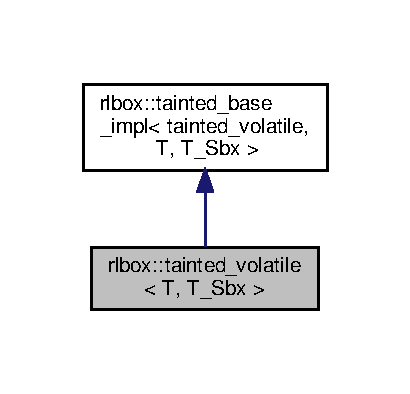
\includegraphics[width=197pt]{classrlbox_1_1tainted__volatile__inherit__graph}
\end{center}
\end{figure}


Collaboration diagram for rlbox\+:\+:tainted\+\_\+volatile$<$ T, T\+\_\+\+Sbx $>$\+:
\nopagebreak
\begin{figure}[H]
\begin{center}
\leavevmode
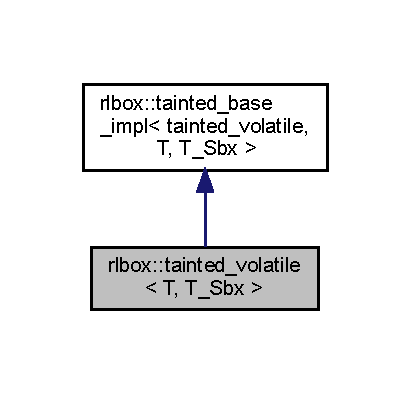
\includegraphics[width=197pt]{classrlbox_1_1tainted__volatile__coll__graph}
\end{center}
\end{figure}
\subsection*{Public Member Functions}
\begin{DoxyCompactItemize}
\item 
\mbox{\Hypertarget{classrlbox_1_1tainted__volatile_a6cfb61db0c20522d8f9f33d111ae4d5c}\label{classrlbox_1_1tainted__volatile_a6cfb61db0c20522d8f9f33d111ae4d5c}} 
\hyperlink{classrlbox_1_1tainted}{tainted}$<$ const T $\ast$, T\+\_\+\+Sbx $>$ {\bfseries operator \&} () const noexcept
\item 
\mbox{\Hypertarget{classrlbox_1_1tainted__volatile_ace5c231dd34dd457c5780711f659a262}\label{classrlbox_1_1tainted__volatile_ace5c231dd34dd457c5780711f659a262}} 
\hyperlink{classrlbox_1_1tainted}{tainted}$<$ T $\ast$, T\+\_\+\+Sbx $>$ {\bfseries operator \&} () noexcept
\item 
\mbox{\Hypertarget{classrlbox_1_1tainted__volatile_a03de23a9e3db2a7ec1c392544c704988}\label{classrlbox_1_1tainted__volatile_a03de23a9e3db2a7ec1c392544c704988}} 
{\footnotesize template$<$typename T\+\_\+\+Rhs\+Ref $>$ }\\\hyperlink{classrlbox_1_1tainted__volatile}{tainted\+\_\+volatile}$<$ T, T\+\_\+\+Sbx $>$ \& {\bfseries operator=} (T\+\_\+\+Rhs\+Ref \&\&val)
\item 
\mbox{\Hypertarget{classrlbox_1_1tainted__volatile_adc112be01be78aff6187e845e2e3ee5f}\label{classrlbox_1_1tainted__volatile_adc112be01be78aff6187e845e2e3ee5f}} 
{\footnotesize template$<$typename T\+\_\+\+Rhs $>$ }\\void {\bfseries assign\+\_\+raw\+\_\+pointer} (\hyperlink{classrlbox_1_1rlbox__sandbox}{rlbox\+\_\+sandbox}$<$ T\+\_\+\+Sbx $>$ \&sandbox, T\+\_\+\+Rhs val)
\item 
\mbox{\Hypertarget{classrlbox_1_1tainted__volatile_a7edbf4fa582a5cedd158b9fe3d1d69b5}\label{classrlbox_1_1tainted__volatile_a7edbf4fa582a5cedd158b9fe3d1d69b5}} 
{\footnotesize template$<$typename T\+\_\+\+Rhs $>$ }\\\hyperlink{classrlbox_1_1tainted__boolean__hint}{tainted\+\_\+boolean\+\_\+hint} \hyperlink{classrlbox_1_1tainted__volatile_a7edbf4fa582a5cedd158b9fe3d1d69b5}{operator==} (T\+\_\+\+Rhs \&\&arg) const
\begin{DoxyCompactList}\small\item\em Comparisons with a \hyperlink{classrlbox_1_1tainted__volatile}{tainted\+\_\+volatile} return only a \char`\"{}hint\char`\"{} to the right answer, i.\+e., something that could be wrong or change. This is because a compromised sandbox can modify \hyperlink{classrlbox_1_1tainted__volatile}{tainted\+\_\+volatile} data at any time. \end{DoxyCompactList}\item 
\mbox{\Hypertarget{classrlbox_1_1tainted__volatile_ad6b318608ffa3306c230b8043b33091d}\label{classrlbox_1_1tainted__volatile_ad6b318608ffa3306c230b8043b33091d}} 
{\footnotesize template$<$typename T\+\_\+\+Dummy  = void$>$ }\\{\bfseries operator bool} () const
\end{DoxyCompactItemize}
\subsection*{Public Attributes}
\begin{DoxyCompactItemize}
\item 
\mbox{\Hypertarget{classrlbox_1_1tainted__volatile_a41f8c034554f4dff986b2209bdc45b4e}\label{classrlbox_1_1tainted__volatile_a41f8c034554f4dff986b2209bdc45b4e}} 
rlbox\+\_\+detail\+\_\+forward\+\_\+binop\+\_\+to\+\_\+base \& {\bfseries T\+\_\+\+Class\+Base}
\end{DoxyCompactItemize}


\subsection{Detailed Description}
\subsubsection*{template$<$typename T, typename T\+\_\+\+Sbx$>$\newline
class rlbox\+::tainted\+\_\+volatile$<$ T, T\+\_\+\+Sbx $>$}

Tainted volatile values are like tainted values but still point to sandbox memory. Dereferencing a tainted pointer produces a \hyperlink{classrlbox_1_1tainted__volatile}{tainted\+\_\+volatile}. 

The documentation for this class was generated from the following file\+:\begin{DoxyCompactItemize}
\item 
/home/shr/\+Code/\+Library\+Sandboxing/rlbox\+\_\+api\+\_\+cpp17/code/include/rlbox.\+hpp\end{DoxyCompactItemize}

\hypertarget{structrlbox_1_1detail_1_1detail__rlbox__is__tainted__boolean__hint_1_1unwrapper}{}\doxysection{rlbox\+::detail\+::detail\+\_\+rlbox\+\_\+is\+\_\+tainted\+\_\+boolean\+\_\+hint\+::unwrapper$<$ T $>$ Struct Template Reference}
\label{structrlbox_1_1detail_1_1detail__rlbox__is__tainted__boolean__hint_1_1unwrapper}\index{rlbox::detail::detail\_rlbox\_is\_tainted\_boolean\_hint::unwrapper$<$ T $>$@{rlbox::detail::detail\_rlbox\_is\_tainted\_boolean\_hint::unwrapper$<$ T $>$}}


Inheritance diagram for rlbox\+::detail\+::detail\+\_\+rlbox\+\_\+is\+\_\+tainted\+\_\+boolean\+\_\+hint\+::unwrapper$<$ T $>$\+:
\nopagebreak
\begin{figure}[H]
\begin{center}
\leavevmode
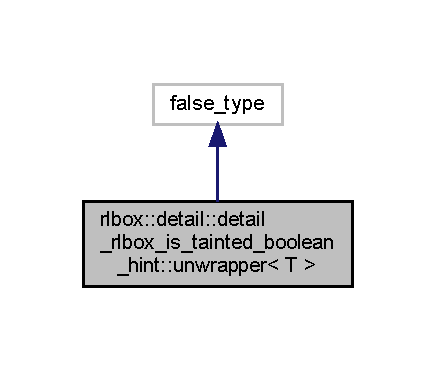
\includegraphics[width=224pt]{structrlbox_1_1detail_1_1detail__rlbox__is__tainted__boolean__hint_1_1unwrapper__inherit__graph}
\end{center}
\end{figure}


Collaboration diagram for rlbox\+::detail\+::detail\+\_\+rlbox\+\_\+is\+\_\+tainted\+\_\+boolean\+\_\+hint\+::unwrapper$<$ T $>$\+:
\nopagebreak
\begin{figure}[H]
\begin{center}
\leavevmode
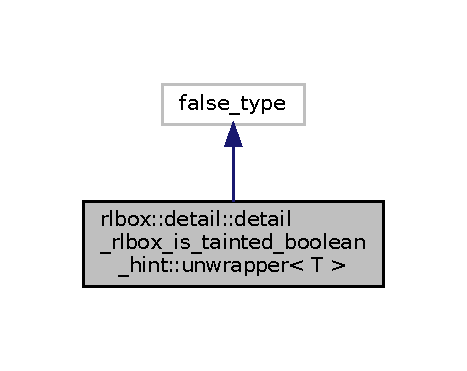
\includegraphics[width=224pt]{structrlbox_1_1detail_1_1detail__rlbox__is__tainted__boolean__hint_1_1unwrapper__coll__graph}
\end{center}
\end{figure}


The documentation for this struct was generated from the following file\+:\begin{DoxyCompactItemize}
\item 
/home/d/hack/rlbox\+\_\+sandboxing\+\_\+api/code/include/rlbox\+\_\+wrapper\+\_\+traits.\+hpp\end{DoxyCompactItemize}

\hypertarget{structrlbox_1_1detail_1_1detail__rlbox__remove__wrapper_1_1unwrapper}{}\doxysection{rlbox\+::detail\+::detail\+\_\+rlbox\+\_\+remove\+\_\+wrapper\+::unwrapper$<$ T $>$ Struct Template Reference}
\label{structrlbox_1_1detail_1_1detail__rlbox__remove__wrapper_1_1unwrapper}\index{rlbox::detail::detail\_rlbox\_remove\_wrapper::unwrapper$<$ T $>$@{rlbox::detail::detail\_rlbox\_remove\_wrapper::unwrapper$<$ T $>$}}
\doxysubsection*{Public Types}
\begin{DoxyCompactItemize}
\item 
\mbox{\Hypertarget{structrlbox_1_1detail_1_1detail__rlbox__remove__wrapper_1_1unwrapper_a880e2c32e27505ebf9e71b896b586c37}\label{structrlbox_1_1detail_1_1detail__rlbox__remove__wrapper_1_1unwrapper_a880e2c32e27505ebf9e71b896b586c37}} 
using {\bfseries type} = T
\item 
\mbox{\Hypertarget{structrlbox_1_1detail_1_1detail__rlbox__remove__wrapper_1_1unwrapper_ac48201968ef70435a4da5ce89e8993f7}\label{structrlbox_1_1detail_1_1detail__rlbox__remove__wrapper_1_1unwrapper_ac48201968ef70435a4da5ce89e8993f7}} 
using {\bfseries type\+\_\+sbx} = void
\end{DoxyCompactItemize}


The documentation for this struct was generated from the following file\+:\begin{DoxyCompactItemize}
\item 
/home/shr/\+Code/\+Library\+Sandboxing/rlbox\+\_\+api\+\_\+cpp17/code/include/rlbox\+\_\+wrapper\+\_\+traits.\+hpp\end{DoxyCompactItemize}

\hypertarget{structrlbox_1_1detail_1_1detail__rlbox__remove__wrapper_1_1unwrapper_3_01sandbox__callback_3_01T_00_01T__Sbx_01_4_01_4}{}\section{rlbox\+:\+:detail\+:\+:detail\+\_\+rlbox\+\_\+remove\+\_\+wrapper\+:\+:unwrapper$<$ sandbox\+\_\+callback$<$ T, T\+\_\+\+Sbx $>$ $>$ Struct Template Reference}
\label{structrlbox_1_1detail_1_1detail__rlbox__remove__wrapper_1_1unwrapper_3_01sandbox__callback_3_01T_00_01T__Sbx_01_4_01_4}\index{rlbox\+::detail\+::detail\+\_\+rlbox\+\_\+remove\+\_\+wrapper\+::unwrapper$<$ sandbox\+\_\+callback$<$ T, T\+\_\+\+Sbx $>$ $>$@{rlbox\+::detail\+::detail\+\_\+rlbox\+\_\+remove\+\_\+wrapper\+::unwrapper$<$ sandbox\+\_\+callback$<$ T, T\+\_\+\+Sbx $>$ $>$}}
\subsection*{Public Types}
\begin{DoxyCompactItemize}
\item 
\mbox{\Hypertarget{structrlbox_1_1detail_1_1detail__rlbox__remove__wrapper_1_1unwrapper_3_01sandbox__callback_3_01T_00_01T__Sbx_01_4_01_4_a0dcaa696c32e68cdf01ac6d9e6e3563f}\label{structrlbox_1_1detail_1_1detail__rlbox__remove__wrapper_1_1unwrapper_3_01sandbox__callback_3_01T_00_01T__Sbx_01_4_01_4_a0dcaa696c32e68cdf01ac6d9e6e3563f}} 
using {\bfseries type} = T
\item 
\mbox{\Hypertarget{structrlbox_1_1detail_1_1detail__rlbox__remove__wrapper_1_1unwrapper_3_01sandbox__callback_3_01T_00_01T__Sbx_01_4_01_4_a2bc8b3468e02fa4b270a5f995f427afe}\label{structrlbox_1_1detail_1_1detail__rlbox__remove__wrapper_1_1unwrapper_3_01sandbox__callback_3_01T_00_01T__Sbx_01_4_01_4_a2bc8b3468e02fa4b270a5f995f427afe}} 
using {\bfseries type\+\_\+sbx} = T\+\_\+\+Sbx
\end{DoxyCompactItemize}


The documentation for this struct was generated from the following file\+:\begin{DoxyCompactItemize}
\item 
/home/shr/\+Code/\+Library\+Sandboxing/rlbox\+\_\+api\+\_\+cpp17/code/include/rlbox\+\_\+wrapper\+\_\+traits.\+hpp\end{DoxyCompactItemize}

\hypertarget{structrlbox_1_1detail_1_1detail__rlbox__remove__wrapper_1_1unwrapper_3_01tainted_3_01T_00_01T__Sbx_01_4_01_4}{}\doxysection{rlbox\+::detail\+::detail\+\_\+rlbox\+\_\+remove\+\_\+wrapper\+::unwrapper\texorpdfstring{$<$}{<} tainted\texorpdfstring{$<$}{<} T, T\+\_\+\+Sbx \texorpdfstring{$>$}{>} \texorpdfstring{$>$}{>} Struct Template Reference}
\label{structrlbox_1_1detail_1_1detail__rlbox__remove__wrapper_1_1unwrapper_3_01tainted_3_01T_00_01T__Sbx_01_4_01_4}\index{rlbox::detail::detail\_rlbox\_remove\_wrapper::unwrapper$<$ tainted$<$ T, T\_Sbx $>$ $>$@{rlbox::detail::detail\_rlbox\_remove\_wrapper::unwrapper$<$ tainted$<$ T, T\_Sbx $>$ $>$}}
\doxysubsection*{Public Types}
\begin{DoxyCompactItemize}
\item 
\mbox{\Hypertarget{structrlbox_1_1detail_1_1detail__rlbox__remove__wrapper_1_1unwrapper_3_01tainted_3_01T_00_01T__Sbx_01_4_01_4_ace6e380e9e64a1681492c3a4f93f3cf5}\label{structrlbox_1_1detail_1_1detail__rlbox__remove__wrapper_1_1unwrapper_3_01tainted_3_01T_00_01T__Sbx_01_4_01_4_ace6e380e9e64a1681492c3a4f93f3cf5}} 
using {\bfseries type} = T
\item 
\mbox{\Hypertarget{structrlbox_1_1detail_1_1detail__rlbox__remove__wrapper_1_1unwrapper_3_01tainted_3_01T_00_01T__Sbx_01_4_01_4_ac91e2c99e60e54c181ccce11433741ec}\label{structrlbox_1_1detail_1_1detail__rlbox__remove__wrapper_1_1unwrapper_3_01tainted_3_01T_00_01T__Sbx_01_4_01_4_ac91e2c99e60e54c181ccce11433741ec}} 
using {\bfseries type\+\_\+sbx} = T\+\_\+\+Sbx
\end{DoxyCompactItemize}


The documentation for this struct was generated from the following file\+:\begin{DoxyCompactItemize}
\item 
/home/d/hack/rlbox\+\_\+sandboxing\+\_\+api/code/include/rlbox\+\_\+wrapper\+\_\+traits.\+hpp\end{DoxyCompactItemize}

\hypertarget{structrlbox_1_1detail_1_1detail__rlbox__is__tainted__boolean__hint_1_1unwrapper_3_01tainted__boolean__hint_01_4}{}\section{rlbox\+:\+:detail\+:\+:detail\+\_\+rlbox\+\_\+is\+\_\+tainted\+\_\+boolean\+\_\+hint\+:\+:unwrapper$<$ tainted\+\_\+boolean\+\_\+hint $>$ Struct Template Reference}
\label{structrlbox_1_1detail_1_1detail__rlbox__is__tainted__boolean__hint_1_1unwrapper_3_01tainted__boolean__hint_01_4}\index{rlbox\+::detail\+::detail\+\_\+rlbox\+\_\+is\+\_\+tainted\+\_\+boolean\+\_\+hint\+::unwrapper$<$ tainted\+\_\+boolean\+\_\+hint $>$@{rlbox\+::detail\+::detail\+\_\+rlbox\+\_\+is\+\_\+tainted\+\_\+boolean\+\_\+hint\+::unwrapper$<$ tainted\+\_\+boolean\+\_\+hint $>$}}


Inheritance diagram for rlbox\+:\+:detail\+:\+:detail\+\_\+rlbox\+\_\+is\+\_\+tainted\+\_\+boolean\+\_\+hint\+:\+:unwrapper$<$ tainted\+\_\+boolean\+\_\+hint $>$\+:
\nopagebreak
\begin{figure}[H]
\begin{center}
\leavevmode
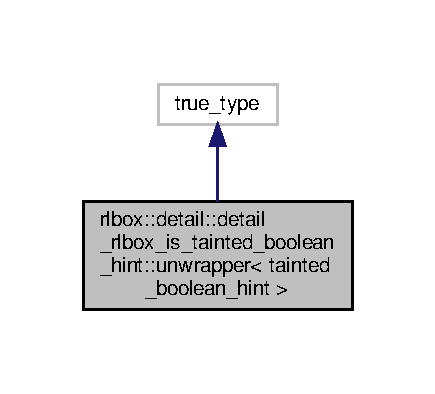
\includegraphics[width=209pt]{structrlbox_1_1detail_1_1detail__rlbox__is__tainted__boolean__hint_1_1unwrapper_3_01tainted__boolean__hint_01_4__inherit__graph}
\end{center}
\end{figure}


Collaboration diagram for rlbox\+:\+:detail\+:\+:detail\+\_\+rlbox\+\_\+is\+\_\+tainted\+\_\+boolean\+\_\+hint\+:\+:unwrapper$<$ tainted\+\_\+boolean\+\_\+hint $>$\+:
\nopagebreak
\begin{figure}[H]
\begin{center}
\leavevmode
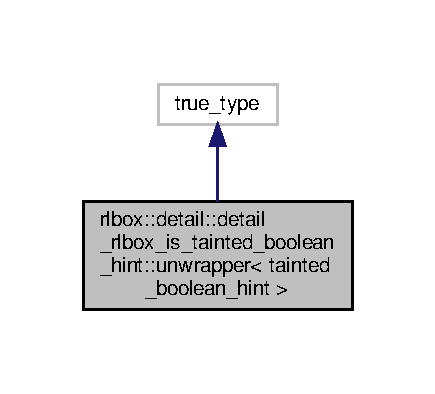
\includegraphics[width=209pt]{structrlbox_1_1detail_1_1detail__rlbox__is__tainted__boolean__hint_1_1unwrapper_3_01tainted__boolean__hint_01_4__coll__graph}
\end{center}
\end{figure}


The documentation for this struct was generated from the following file\+:\begin{DoxyCompactItemize}
\item 
/home/shr/\+Code/\+Library\+Sandboxing/rlbox\+\_\+api\+\_\+cpp17/code/include/rlbox\+\_\+wrapper\+\_\+traits.\+hpp\end{DoxyCompactItemize}

\hypertarget{structrlbox_1_1detail_1_1detail__rlbox__remove__wrapper_1_1unwrapper_3_01tainted__opaque_3_01T_00_01T__Sbx_01_4_01_4}{}\doxysection{rlbox\+::detail\+::detail\+\_\+rlbox\+\_\+remove\+\_\+wrapper\+::unwrapper$<$ tainted\+\_\+opaque$<$ T, T\+\_\+\+Sbx $>$ $>$ Struct Template Reference}
\label{structrlbox_1_1detail_1_1detail__rlbox__remove__wrapper_1_1unwrapper_3_01tainted__opaque_3_01T_00_01T__Sbx_01_4_01_4}\index{rlbox::detail::detail\_rlbox\_remove\_wrapper::unwrapper$<$ tainted\_opaque$<$ T, T\_Sbx $>$ $>$@{rlbox::detail::detail\_rlbox\_remove\_wrapper::unwrapper$<$ tainted\_opaque$<$ T, T\_Sbx $>$ $>$}}
\doxysubsection*{Public Types}
\begin{DoxyCompactItemize}
\item 
\mbox{\Hypertarget{structrlbox_1_1detail_1_1detail__rlbox__remove__wrapper_1_1unwrapper_3_01tainted__opaque_3_01T_00_01T__Sbx_01_4_01_4_ad138d193f218b44c9b5ea938447673c8}\label{structrlbox_1_1detail_1_1detail__rlbox__remove__wrapper_1_1unwrapper_3_01tainted__opaque_3_01T_00_01T__Sbx_01_4_01_4_ad138d193f218b44c9b5ea938447673c8}} 
using {\bfseries type} = T
\item 
\mbox{\Hypertarget{structrlbox_1_1detail_1_1detail__rlbox__remove__wrapper_1_1unwrapper_3_01tainted__opaque_3_01T_00_01T__Sbx_01_4_01_4_a74334bbae27eacae858c7bf841e8cb25}\label{structrlbox_1_1detail_1_1detail__rlbox__remove__wrapper_1_1unwrapper_3_01tainted__opaque_3_01T_00_01T__Sbx_01_4_01_4_a74334bbae27eacae858c7bf841e8cb25}} 
using {\bfseries type\+\_\+sbx} = T\+\_\+\+Sbx
\end{DoxyCompactItemize}


The documentation for this struct was generated from the following file\+:\begin{DoxyCompactItemize}
\item 
/home/d/hack/rlbox\+\_\+sandboxing\+\_\+api/code/include/rlbox\+\_\+wrapper\+\_\+traits.\+hpp\end{DoxyCompactItemize}

\hypertarget{structrlbox_1_1detail_1_1detail__rlbox__remove__wrapper_1_1unwrapper_3_01tainted__volatile_3_01T_00_01T__Sbx_01_4_01_4}{}\section{rlbox\+:\+:detail\+:\+:detail\+\_\+rlbox\+\_\+remove\+\_\+wrapper\+:\+:unwrapper$<$ tainted\+\_\+volatile$<$ T, T\+\_\+\+Sbx $>$ $>$ Struct Template Reference}
\label{structrlbox_1_1detail_1_1detail__rlbox__remove__wrapper_1_1unwrapper_3_01tainted__volatile_3_01T_00_01T__Sbx_01_4_01_4}\index{rlbox\+::detail\+::detail\+\_\+rlbox\+\_\+remove\+\_\+wrapper\+::unwrapper$<$ tainted\+\_\+volatile$<$ T, T\+\_\+\+Sbx $>$ $>$@{rlbox\+::detail\+::detail\+\_\+rlbox\+\_\+remove\+\_\+wrapper\+::unwrapper$<$ tainted\+\_\+volatile$<$ T, T\+\_\+\+Sbx $>$ $>$}}
\subsection*{Public Types}
\begin{DoxyCompactItemize}
\item 
\mbox{\Hypertarget{structrlbox_1_1detail_1_1detail__rlbox__remove__wrapper_1_1unwrapper_3_01tainted__volatile_3_01T_00_01T__Sbx_01_4_01_4_a35e2bbef854da26ac6183d86973088d1}\label{structrlbox_1_1detail_1_1detail__rlbox__remove__wrapper_1_1unwrapper_3_01tainted__volatile_3_01T_00_01T__Sbx_01_4_01_4_a35e2bbef854da26ac6183d86973088d1}} 
using {\bfseries type} = T
\item 
\mbox{\Hypertarget{structrlbox_1_1detail_1_1detail__rlbox__remove__wrapper_1_1unwrapper_3_01tainted__volatile_3_01T_00_01T__Sbx_01_4_01_4_a03486bcca1d3277cdfab50c85839b595}\label{structrlbox_1_1detail_1_1detail__rlbox__remove__wrapper_1_1unwrapper_3_01tainted__volatile_3_01T_00_01T__Sbx_01_4_01_4_a03486bcca1d3277cdfab50c85839b595}} 
using {\bfseries type\+\_\+sbx} = T\+\_\+\+Sbx
\end{DoxyCompactItemize}


The documentation for this struct was generated from the following file\+:\begin{DoxyCompactItemize}
\item 
/home/shr/\+Code/\+Library\+Sandboxing/rlbox\+\_\+api\+\_\+cpp17/code/include/rlbox\+\_\+wrapper\+\_\+traits.\+hpp\end{DoxyCompactItemize}

\hypertarget{structrlbox_1_1detail_1_1std__array__to__c__arr__detail_1_1W}{}\doxysection{rlbox\+::detail\+::std\+\_\+array\+\_\+to\+\_\+c\+\_\+arr\+\_\+detail\+::W\texorpdfstring{$<$}{<} T \texorpdfstring{$>$}{>} Struct Template Reference}
\label{structrlbox_1_1detail_1_1std__array__to__c__arr__detail_1_1W}\index{rlbox::detail::std\_array\_to\_c\_arr\_detail::W$<$ T $>$@{rlbox::detail::std\_array\_to\_c\_arr\_detail::W$<$ T $>$}}
\doxysubsection*{Public Types}
\begin{DoxyCompactItemize}
\item 
\mbox{\Hypertarget{structrlbox_1_1detail_1_1std__array__to__c__arr__detail_1_1W_a0820ff0c6b9407092672b903661c9459}\label{structrlbox_1_1detail_1_1std__array__to__c__arr__detail_1_1W_a0820ff0c6b9407092672b903661c9459}} 
using {\bfseries type} = T
\end{DoxyCompactItemize}


The documentation for this struct was generated from the following file\+:\begin{DoxyCompactItemize}
\item 
/home/d/hack/rlbox\+\_\+sandboxing\+\_\+api/code/include/rlbox\+\_\+type\+\_\+traits.\+hpp\end{DoxyCompactItemize}

\hypertarget{structrlbox_1_1detail_1_1std__array__el__detail_1_1W}{}\doxysection{rlbox\+::detail\+::std\+\_\+array\+\_\+el\+\_\+detail\+::W\texorpdfstring{$<$}{<} T \texorpdfstring{$>$}{>} Struct Template Reference}
\label{structrlbox_1_1detail_1_1std__array__el__detail_1_1W}\index{rlbox::detail::std\_array\_el\_detail::W$<$ T $>$@{rlbox::detail::std\_array\_el\_detail::W$<$ T $>$}}
\doxysubsection*{Public Types}
\begin{DoxyCompactItemize}
\item 
\mbox{\Hypertarget{structrlbox_1_1detail_1_1std__array__el__detail_1_1W_a40a0b72602d7250352c6adc3947e8ccc}\label{structrlbox_1_1detail_1_1std__array__el__detail_1_1W_a40a0b72602d7250352c6adc3947e8ccc}} 
using {\bfseries type} = T
\end{DoxyCompactItemize}


The documentation for this struct was generated from the following file\+:\begin{DoxyCompactItemize}
\item 
/home/d/hack/rlbox\+\_\+sandboxing\+\_\+api/code/include/rlbox\+\_\+type\+\_\+traits.\+hpp\end{DoxyCompactItemize}

%--- End generated contents ---

% Index
\backmatter
\newpage
\phantomsection
\clearemptydoublepage
\addcontentsline{toc}{chapter}{Index}
\printindex

\end{document}
